%%%%%%%%%%%%%%%%%%%%%%%%%%%%%%%%%%%%%%%%%
% Masters/Doctoral Thesis 
% LaTeX Template
% Version 2.4 (22/11/16)
%
% This template has been downloaded from:
% http://www.LaTeXTemplates.com
%
% Version 2.x major modifications by:
% Vel (vel@latextemplates.com)
%
% This template is based on a template by:
% Steve Gunn (http://users.ecs.soton.ac.uk/srg/softwaretools/document/templates/)
% Sunil Patel (http://www.sunilpatel.co.uk/thesis-template/)
%
% Template license:
% CC BY-NC-SA 3.0 (http://creativecommons.org/licenses/by-nc-sa/3.0/)
%
%%%%%%%%%%%%%%%%%%%%%%%%%%%%%%%%%%%%%%%%%

%----------------------------------------------------------------------------------------
%	PACKAGES AND OTHER DOCUMENT CONFIGURATIONS
%----------------------------------------------------------------------------------------

\documentclass[
11pt, % The default document font size, options: 10pt, 11pt, 12pt
%oneside, % Two side (alternating margins) for binding by default, uncomment to switch to one side
catalan, % ngerman for German
singlespacing, % Single line spacing, alternatives: onehalfspacing or doublespacing
%draft, % Uncomment to enable draft mode (no pictures, no links, overfull hboxes indicated)
%nolistspacing, % If the document is onehalfspacing or doublespacing, uncomment this to set spacing in lists to single
%liststotoc, % Uncomment to add the list of figures/tables/etc to the table of contents
%toctotoc, % Uncomment to add the main table of contents to the table of contents
%parskip, % Uncomment to add space between paragraphs
%nohyperref, % Uncomment to not load the hyperref package
headsepline, % Uncomment to get a line under the header
%chapterinoneline, % Uncomment to place the chapter title next to the number on one line
%consistentlayout, % Uncomment to change the layout of the declaration, abstract and acknowledgements pages to match the default layout
]{MastersDoctoralThesis} % The class file specifying the document structure

\usepackage{eurosym}
\usepackage[utf8]{inputenc} % Required for inputting international characters
\usepackage[T1]{fontenc} % Output font encoding for international characters
\usepackage{booktabs}
\usepackage{palatino} % Use the Palatino font by default

\usepackage[backend=bibtex,style=authoryear,natbib=true]{biblatex} % Use the bibtex backend with the authoryear citation style (which resembles APA)

\addbibresource{example.bib} % The filename of the bibliography

\usepackage[autostyle=true]{csquotes} % Required to generate language-dependent quotes in the bibliography

%----------------------------------------------------------------------------------------
%	MARGIN SETTINGS
%----------------------------------------------------------------------------------------

\geometry{
	paper=a4paper, % Change to letterpaper for US letter
	inner=2.5cm, % Inner margin
	outer=3.8cm, % Outer margin
	bindingoffset=.5cm, % Binding offset
	top=1.5cm, % Top margin
	bottom=1.5cm, % Bottom margin
	%showframe, % Uncomment to show how the type block is set on the page
}

%----------------------------------------------------------------------------------------
%	THESIS INFORMATION
%----------------------------------------------------------------------------------------

\thesistitle{WildTraveling} % Your thesis title, this is used in the title and abstract, print it elsewhere with \ttitle
\supervisor{Clàudia Ayala Martínez} % Your supervisor's name, this is used in the title page, print it elsewhere with \supname
\examiner{} % Your examiner's name, this is not currently used anywhere in the template, print it elsewhere with \examname
\degree{Grau en Enginyeria Informàtica} % Your degree name, this is used in the title page and abstract, print it elsewhere with \degreename
\author{Pere Bergé Sànchez} % Your name, this is used in the title page and abstract, print it elsewhere with \authorname
\addresses{} % Your address, this is not currently used anywhere in the template, print it elsewhere with \addressname

\subject{Biological Sciences} % Your subject area, this is not currently used anywhere in the template, print it elsewhere with \subjectname
\keywords{} % Keywords for your thesis, this is not currently used anywhere in the template, print it elsewhere with \keywordnames
\university{\href{http://www.upc.edu}{Universitat Politècnica de Catalunya}} % Your university's name and URL, this is used in the title page and abstract, print it elsewhere with \univname
\department{\href{https://www.fib.upc.edu/}{Enginyeria del Software i Sistemes d'Informació}} % Your department's name and URL, this is used in the title page and abstract, print it elsewhere with \deptname
\group{\href{http://researchgroup.university.com}{Research Group Name}} % Your research group's name and URL, this is used in the title page, print it elsewhere with \groupname
\faculty{\href{https://www.fib.upc.edu/}{Facultat d'informàtica de Catalunya}} % Your faculty's name and URL, this is used in the title page and abstract, print it elsewhere with \facname

\AtBeginDocument{
\hypersetup{pdftitle=\ttitle} % Set the PDF's title to your title
\hypersetup{pdfauthor=\authorname} % Set the PDF's author to your name
\hypersetup{pdfkeywords=\keywordnames} % Set the PDF's keywords to your keywords
}

\begin{document}

\frontmatter % Use roman page numbering style (i, ii, iii, iv...) for the pre-content pages

\pagestyle{plain} % Default to the plain heading style until the thesis style is called for the body content

%----------------------------------------------------------------------------------------
%	TITLE PAGE
%----------------------------------------------------------------------------------------

\begin{titlepage}
\begin{center}

\vspace*{.06\textheight}
{\scshape\LARGE \univname\par}\vspace{1.5cm} % University name
\textsc{\Large TREBALL FINAL DE GRAU}\\[0.5cm] % Thesis type

\HRule \\[0.4cm] % Horizontal line
{\huge \bfseries \ttitle\par}\vspace{0.4cm} % Thesis title
Informe de Seguiment
\HRule \\[1.5cm] % Horizontal line
 
\begin{minipage}[t]{0.4\textwidth}
\begin{flushleft} \large
\emph{Autor:}\\
\href{http://www.johnsmith.com}{\authorname} % Author name - remove the \href bracket to remove the link
\end{flushleft}
\end{minipage}
\begin{minipage}[t]{0.4\textwidth}
\begin{flushright} \large
\emph{Tutora:} \\
\href{http://www.jamessmith.com}{\supname} % Supervisor name - remove the \href bracket to remove the link  
\end{flushright}
\end{minipage}\\[3cm]
 
\vfill

\large \degreename\\[0.3cm] % University requirement text
\large Facultat d'Informàtica de Barcelona\\ % University requirement text
\deptname\\[2cm] % Research group name and department name
 
\vfill

{\large \today}\\[4cm] % Date
%\includegraphics{Logo} % University/department logo - uncomment to place it
 
\vfill
\end{center}
\end{titlepage}

%----------------------------------------------------------------------------------------
%	LIST OF CONTENTS/FIGURES/TABLES PAGES
%----------------------------------------------------------------------------------------

\tableofcontents % Prints the main table of contents

%----------------------------------------------------------------------------------------
%	THESIS CONTENT - CHAPTERS
%----------------------------------------------------------------------------------------

\mainmatter % Begin numeric (1,2,3...) page numbering

\pagestyle{thesis} % Return the page headers back to the "thesis" style

% Include the chapters of the thesis as separate files from the Chapters folder
% Uncomment the lines as you write the chapters

% Chapter Template

\chapter{Introducció i estat de l'art} % Main chapter title

\label{Context} % Change X to a consecutive number; for referencing this chapter elsewhere, use \ref{ChapterX}

Aquest projecte és un Treball Final de Grau de l'especialitat d'Enginyeria del Software de la Facultat d'Informàtica de Barcelona (Universitat Politècnica de Catalunya). Es tracta d'un projecte de modalitat A que pretén crear una aplicació de suport al viatger.

%----------------------------------------------------------------------------------------

\section{Formulació del problema}

Viatjar ajuda a veure la vida des de perspectives diverses, aquest és un dels motius pels quals cada dia tothom està més disposat a emprendre viatges arreu del món. Existeixen molts perfils diferents de viatgers, a alguns els agrada descobrir natura, a d’altres les grans ciutats, hi ha qui es decanta per la tranquilitat i qui prefereix l’aventura. Sigui quin sigui l’enfoc del viatge, el propòsit és aprendre alguna cosa que quedi per al record.\\

En els darrers anys, com a conseqüència d’internet i l’abaratiment de les companyies low cost, és molt més fàcil desplaçar-se i estar informat sobre els diferents racons del món. És important també tenir en compte que la gran majoria de gent disposa d’un smartphone, aquest fet permet al viatger accedir a internet durant el viatge i, per tant, estar connectat constantment, cosa que simplifica molt l’accés a informació al moment.\\

Les persones ens adaptem molt ràpidament a les coses que ens són més fàcils de fer, per aquest motiu actualment no es planifica tant i sovint es necessita una eina que permeti solucionar un problema a l’instant. És en aquest context on apareix l’aplicació que pretén desenvolupar aquest projecte.\\

Durant un viatge sorgeixen moltes necessitats com poden ser: buscar un restaurant, informar-se del temps, buscar transport, portar un control de les despeses, etc. Actualment existeixen varies aplicacions que ataquen parts concretes d’aquest problema però això obliga al viatger a tenir moltes aplicacions instal·lades al seu dispositiu sense comunicació entre elles.\\

La idea que proposa aquest projecte és construir una aplicació que englobi les funcionalitats que un viatger considera més importants durant el transcurs del seu viatge presentant-li la informació filtrada tenint en compte el seu estil de viatjar. D’aquesta manera podem definir els objectius del projecte.\\

Aquest projecte té quatre objectius molt clars:
\begin{itemize}
\item{\textbf{Donar suport al viatger durant el transcurs del seu viatge:}} el viatger necessita suport de diversos tipus durant el viatge, per aquest motiu, s’han dut a terme entrevistes a viatgers que han servit per orientar i definir les funcionalitats que vol oferir l’aplicació. Aquestes són: gestió econòmica, previsió metereològica, gestió de cerques de llocs d’interès, gestió d’emergències, cerca de transports, cerca d’imatges i gestió de notes.\\

\item{\textbf{Ser intermediari en l’ús de diverses aplicacions que ajuden al viatger:}} actualment existeixen diverses aplicacions especialitzades en les funcionalitats que aquesta vol implementar. L’objectiu es basa en utilitzar algunes de les aplicacions disponibles en el mercat per tal de crear funcionalitats pròpies i d’aquesta manera obtenir una aplicació completa per al suport al viatger. 

\item{\textbf{Personalitzar les dades obtingudes per a cada viatger:}} qualsevol persona pot emprendre un viatge, per tant, els viatgers no tenen unes preferències establertes, hi ha molta diversitat d’estils. Per aquest motiu aquesta aplicació planteja la personalització dels viatges per tal de filtrar la informació obtinguda a través de l’accés a d’altres aplicacions i així ser capaç d’oferir a l’usuari el que s’ajusta més al seu estil.

\item{\textbf{Ser fàcilment escalable:}} el món de la tecnologia és un món canviant, per aquest motiu aquesta aplicació vol estar preparada per agregar o eliminar funcionalitats de la manera més senzilla possible.

\end{itemize}

\section{Parts interessades}

Aquest projecte va adreçat a satisfer les necessitats d’un sector molt ampli de població, no estem parlant d’un client concret. Les parts interessades poden tenir objectius molt diversos. En aquest projecte definim les següents parts interessades:
\begin{itemize}

\item\textbf{Viatgers}\\
Els viatgers són els principals protagonistes, són els que es beneficien de l’aplicació de forma directa.

\item\textbf{Ajuntaments}\\
Les ciutats obtenen un gran benefici del turisme, per aquest motiu els ajuntaments estan interessats en captar el màxim nombre de turistes possibles. Aquesta aplicació ajuda a donar a conèixer racons amb encant que no surten a les guies convencionals.

\item\textbf{Competència}\\
Les plataformes que tracten el mateix tema es veuen afectades pel desenvolupament d’aquest projecte de forma indirecta. En tenir accés a aquesta nova plataforma tenen l’oportunitat d’innovar en la seva.

\end{itemize}
\section{Estudi de mercat}

En aquest punt s’analitzen les diferents opcions que ofereix el mercat per afrontar el problema descrit.\\
El primer pas ha estat buscar aplicacions similars a la proposada. Després de fer un anàlisi exhaustiu del mercat s’ha conclòs amb la idea de que no existeix una aplicació que s’ajusti a la idea proposada. Sí que es veritat, però, que existeixen aplicacions de suport al viatger durant un viatge com és el cas de Virtual Travel Assistant.
\begin{itemize}
\item{\textbf{Aplicació complerta}}
\begin{itemize}
\item{\textbf{Virtual Travel Assistant\\}}
Virtual Travel Assistant és una aplicació gratuïta que ajuda al viatger durant el transcurs del seu viatge. Aquesta ofereix cerca de llocs d’interès, consell en l’elecció de transport i servei de mapes.\\
Aquesta aplicació, però, té grans diferències amb la proposada. L’aplicació que desenvolupa aquest projecte destaca en la personalització de les cerques i conté més funcionalitats que completen l’aplicació per a que sigui més útil durant el viatge.\\
\end{itemize}

\begin{figure}[!h]
\centering

\includegraphics[scale=0.85]{Figures/vta1.png}
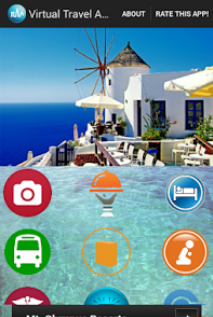
\includegraphics[scale=0.85]{Figures/vta2.png}
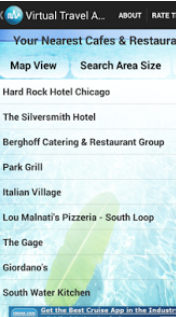
\includegraphics[scale=0.85]{Figures/vta3.png}
\caption{Settle up}
\end{figure}

\end{itemize}

Per tal de fer un millor anàlisi del mercat, s’han analitzat aplicacions especialitzades en les funcionalitats que aquesta vol incorporar i que han sigut anomenades anteriorment.

\begin{itemize}
\item{\textbf{Gestió econòmica}}\\
En aquest punt s’analitza el mercat des del punt de vista de la gestió econòmica del viatge. Existeixen varies aplicacions, totes bastant similars, que tracten aquest tema.
Aquesta funcionalitat pretén ser implementada, per tant , no s’utilitzaran aplicacions existents ja que no acaben d’ajustar-se al perfil desitjat.
S’han analitzat dos aplicacions que s’han escollit tenint en compte les descàrregues i opinions satisfactòries dels usuaris.
\begin{itemize}
\item{\textbf{Settle Up}}\\
Settle Up és una aplicació mòbil que ajuda a portar el control de despeses. Dins les seves característiques destaquen la gestió d’usuari, la gestió de divises i el fet que quan un usuari és inclòs en una nova despesa aquest rep un avís. A més, ofereix l’opció de filtrar les despeses tenint en compte la categoria d’aquesta.

\begin{figure}[!h]
\centering
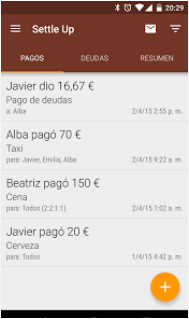
\includegraphics[scale=0.90]{Figures/settleUp1.jpg}
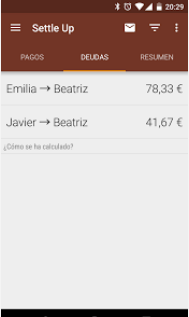
\includegraphics[scale=0.90]{Figures/settleUp2.jpg}
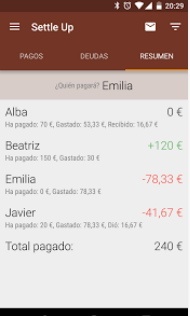
\includegraphics[scale=0.90]{Figures/settleUp3.jpg}
\caption{Settle up}
\end{figure}

\item{\textbf{Splitewise}}\\
Splitewise, aplicació mòbil de control de despeses, ofereix gestió d’usuaris, possibilitat de crear una xarxa d’amics i gestió de divises. En aquesta aplicació també s’hi pot afegir una foto i una categoria a la despesa.

\begin{figure}[!h]
\centering
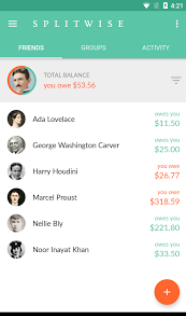
\includegraphics[scale=0.90]{Figures/splitwise1.jpg}
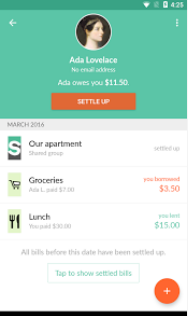
\includegraphics[scale=0.90]{Figures/splitwise2.jpg}
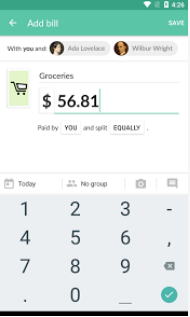
\includegraphics[scale=0.90]{Figures/splitwise3.jpg}
\caption{Splitwise}
\end{figure}

\end{itemize}
\item{\textbf{Previsió metereològica}}\\
En aquest punt s’analitzen les aplicacions de previsió metereològica. Existeixen varies aplicacions molt complertes que controlen la metereologia. Cap d’aquestes, però, està enfocada cap al món viatger, la idea de l’aplicació proposada és mostrar la informació que un viatger necessita saber per decidir què fer durant la seva jornada.\\
S’han analitzat dues aplicacions:
\begin{itemize}
\item{\textbf{Rain Alarm}}\\
Rain Alarm destaca pel seu mapa amb representació gràfica de la probabilitat de pluja a l’instant. També localitza automàticament el punt on es troba l’usuari, avisa en cas de pluja imminent i ofereix l’opció d’ajustar la precisió d’aquest avís. Un dels punts negatius de l’aplicació és que conté publicitat.


\begin{figure}[!h]
\centering
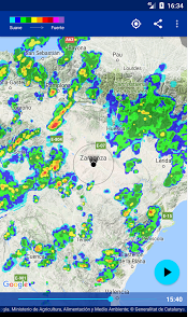
\includegraphics[scale=0.90]{Figures/rainAlarm.jpg}
\caption{Meteoplaza}
\end{figure}

\item{\textbf{Alarma lluvia meteoplaza}}\\
Aquesta aplicació és més simple que l’anterior. Destaca per la representació gràfica de la probabilitat de pluja a l’instant, la localització automàtica i l’avís a l’usuari en cas de pluja imminent.

\begin{figure}[!h]
\centering
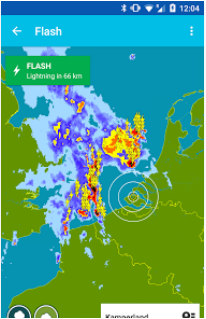
\includegraphics[scale=0.90]{Figures/meteoplaza1.jpg}
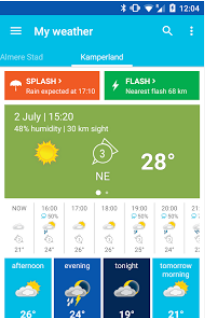
\includegraphics[scale=0.90]{Figures/meteoplaza2.jpg}
\caption{Meteoplaza}
\end{figure}

\end{itemize}
\item{\textbf{Gestió d’emergències}}\\
En aquest punt s’analitzen les aplicacions que tracten el suport en cas d’emergència. L’aplicació que vol crear aquest projecte proposa una funcionalitat que gestioni emergències amb funcionalitats útils per al viatger durant el dia a dia del seu viatge.\\
S’han analitzat dues aplicacions:
\begin{itemize}
\item{\textbf{Emergency Assistant}}\\
Emergency Assistant guarda un perfil personal de l’usuari i emmagatzema contactes a qui acudir en cas d’emergència. Aquestes funcionalitats són les que més s’apropen al que proposa el projecte. A més, també ofereix control d’al·lèrgies, informació sobre l’assegurança, un llistat de medicacions que l’usuari pren i l’historial mèdic. Es considera, però, que aquestes darreres funcionalitats no són prou importants en el context sobre el que es treballa.

\begin{figure}[!h]
\centering
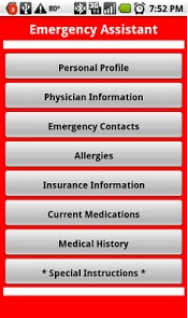
\includegraphics[scale=0.90]{Figures/emerAssistant1.jpg}
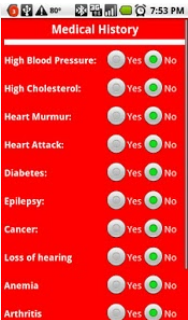
\includegraphics[scale=0.90]{Figures/emerAssistant2.jpg}
\caption{Emergency assistant}
\end{figure}

\item{\textbf{First Call}}\\
First Call ofereix funcionalitats molt interessants pel que fa al punt de vista viatger que té el projecte. Aquesta aplicació és molt més senzilla i es centra en classificar el tipus d’emergència del que es tracta i facilitar molt l’avís a terceres persones en cas d’accident, en aquest cas s’envia un avís a d’altres usuaris de l’aplicació. A més també ofereix informació sobre els telèfons de contacte en cas d’emergència de diferents països.

\clearpage

\begin{figure}[!h]
\centering
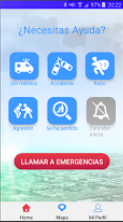
\includegraphics[scale=1.10]{Figures/firstCall1.jpg}
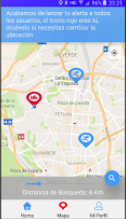
\includegraphics[scale=1.10]{Figures/firstCall2.jpg}
\caption{First Call}
\end{figure}

\end{itemize}
\item{\textbf{Gestió de cerques}}\\
En aquest punt s’analitzen les aplicacions que tenen a veure amb cercar llocs d’interès en un lloc concret.
S’han analitzat les dues aplicacions més utilitzades al moment.
\begin{itemize}
\item{\textbf{Arround me}}\\
Arround me ofereix cerques d’establiments que poden interessar a una persona quan està fora de casa, aquests establiments els ofereix de manera ordenada per categories diferenciant cerca d’hotels, restaurants, gasolineres, etc. A més, també ofereix servei de previsió metereològica.

\begin{figure}[!h]
\centering
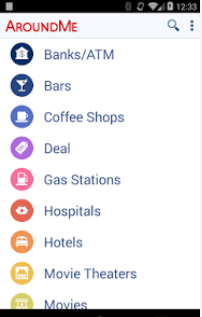
\includegraphics[scale=0.90]{Figures/arroundMe1.jpg}
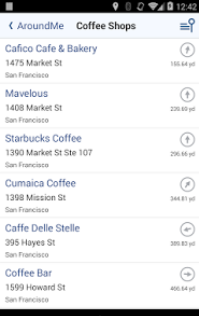
\includegraphics[scale=0.90]{Figures/arroundMe2.jpg}
\caption{Arround me}
\end{figure}

\clearpage

\item{\textbf{Google Maps}}\\
Google Maps és una aplicació molt complerta que ofereix cerques d’establiments, rutes entre un punt i un altre i representació en forma de mapa de tot el món.
D’altra banda, cal dir que cap de les dues aplicacions ofereix una cerca personalitzada per a l’usuari i tampoc està exclusivament enfocat al món viatger. Aquests dos punts són trets distintius d’aquest projecte.



\begin{figure}[!h]
\centering
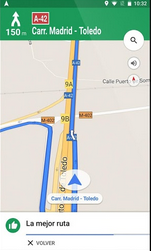
\includegraphics[scale=1.10]{Figures/maps1.jpg}
\caption{Google Maps}
\end{figure}

\end{itemize}
\item{\textbf{Gestió de notes}}\\
En aquest punt s’analitzen les aplicacions que treballen en el camp de les notes escrites. Aquesta funcionalitat no té gairebé res a veure amb el món dels viatges, tot i així es decideix implementar-la ja que es troba interessant oferir un lloc on enregistrar fets curiosos, anècdotes o diferents notes.\\
Existeixen moltes aplicacions que presenten solució a aquest problema, s’han analitzat dues que es considera que es poden apropar a la funcionalitat desitjada.
\begin{itemize}
\item{\textbf{Notes}}\\
Notes és una aplicació gratuïta que ofereix creació de notes amb l’opció d’organitzar-les en carpetes, llistes de verificació i establir recordatoris a la nota. A més, les notes es guarden automàticament quan són creades o modificades. 

\clearpage

\begin{figure}[!h]
\centering
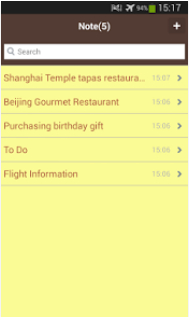
\includegraphics[scale=1.00]{Figures/notes1.jpg}

\includegraphics[scale=0.70]{Figures/notes2.jpg}
\caption{Notes}
\end{figure}

\item{\textbf{ColorNote}}\\
ColorNote és una aplicació simple de llibreta que ofereix organització de notes per color, llistes de verificació i possibilitat de posar contrassenya a les notes. L’aplicació, a més, també té recordatori i la possibilitat de compartir notes a través de SMS i correu electrònic.
L’aplicació que proposa aquest projecte pretén oferir un servei bàsic de notes basat en el que pot necessitar el viatger durant el seu viatge. És per aquest motiu que es vol que cada nota estigui localitzada geogràficament i es pugui etiquetar els viatgers.


\begin{figure}[!h]
\centering
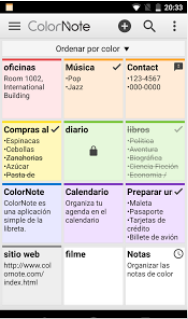
\includegraphics[scale=0.90]{Figures/colorNote1.jpg}
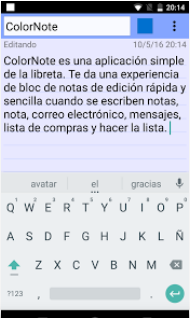
\includegraphics[scale=0.90]{Figures/colorNote2.jpg}
\caption{Color note}
\end{figure}

\end{itemize}
\end{itemize}
\section{Conclusions}
Després d'un anàlisi exhaustiu de la situació actual del mercat pel que fa a aplicacions mòbil que puguin competir amb la idea d'aquest projecte és conclou que realment hi ha un buit en aquest camp.\\

Existeixen, com s'ha exposat en l'apartat anterior, moltes aplicacions que afronten funcionalitats que poden ajudar al viatger durant el trascurs del seu viatge. No obstant, cap d'aquestes aplicacions engloba funcionalitats de vàries temàtiques ni té el món viatger com a temàtica.\\

L'estudi del mercat, ha estat molt útil també, a l'hora de refinar les idees que es tenien sobre que oferir a l'usuari en cada funcionalitat.

% Chapter Template

\chapter{Abast del projecte} % Main chapter title

\label{Abast} % Change X to a consecutive number; for referencing this chapter elsewhere, use \ref{ChapterX}

La idea d’aquest projecte és crear una aplicació referència per qualsevol persona disposada a emprendre un viatge. Una plataforma on trobar suport durant un viatge de qualsevol tipus.\\

L’aplicació ofereix, aprofitant d’altres sistemes ja al mercat, un conjunt de funcionalitats útils a l’hora de viatjar. Les funcionalitats són les següents:
\begin{itemize}
\item{Gestió econòmica:} Controlar qui ha pagat què durant un viatge en grup o bé
el control de les despeses del viatge de manera personal.
\begin{itemize}
\item{}Quan es crea una nova despesa s’envia un avís al deutor.
\item{}Despesa total del viatge.
\end{itemize}
\item{}Gestió de notes: Guardar notes per tal de recordar anècdotes o fets concrets
del viatge.
\begin{itemize}
\item{}Les notes tenen localització geogràfica.
\item{}Possibilitat d’etiquetar viatgers a les notes.
\end{itemize}
\item{}Gestió de cerques: Cerca de llocs d’interès de la zona on està situat l’usuari o de qualsevol altre punt.
\begin{itemize}
\item{}Cerca de restaurants.
\item{}Cerca de bars.
\item{}Cerca de llocs d’interès lúdic.
\item{}Cerca de botigues.
\item{}Cerca de llocs exteriors d’interés.
\item{}Consulta de la ruta fins al punt trobat.
\end{itemize}
Els resultats que s’obtenen de la cerca es mostren a l’usuari ordenats d’acord amb l’estil de viatjar que té l’usuari. Per fer això, abans de començar el viatge, l’aplicació proposa un formulari per tal de descriure el caràcter del viatge. Això dona l’opció al sistema de filtrar les cerques i proposar a l’usuari les opcions més adequades al seu estil.

\item{}Gestió d’emergències: Suport en cas d’emergència tenint en compte el país.
\begin{itemize}
\item{}Ruta fins a l’hospital més proper.
\item{}Trucada al telèfon d’emergències del país.
\item{}Trucada al contacte d’emergències.
\end{itemize}
En aquesta funcionalitat es vol donar la possibilitat a l’usuari de contactar amb una persona de confiança en cas d’emergència. Per aconseguir això, quan s’inicia el viatge, es presenta a l’usuari un formulari on s’han d’introduir el nom, el número de telèfon i el correu electrònic de qui serà la persona de contacte.

\item{}Previsió metereològica: Estar informat de la metereologia en tot moment.
\begin{itemize}
\item{}Predicció setmanal.
\item{}Informació metereològica del dia.
\end{itemize} 
\end{itemize}

\section{Obstacles i riscs}

Per tal d’aconseguir certes funcionalitats de l’aplicació es vol accedir a diferents serveis web per tal d’aconseguir dades concretes. Per una banda, és necessitarà connexió a internet sempre que s’hi vulgui accedir, i per l’altra, el funcionament de l’aplicació depén de la disponibilitat del servei web.\\

En el cas de les trucades d’emergència al telèfon d’emergències del país on estigui el viatger, pot ser que es trobi en un país on no hi ha dades registrades sobre els telèfons d’emergència. Un problema molt semblant pot passar a l’hora d’obtenir llocs d’interés, ja que l’usuari es pot trobar en un lloc on no hi ha cap punt ens molts quilòmetres a la rodona.\\

En ser un Treball Final de Grau té una data límit fixada. Això implica que qualsevol contratemps que faci endarrerir el projecte no es té gaire marge de maniobra per tal d’acabar-lo a temps.\\

Pel que fa a l’ús del sistema, un cop acabat i posat en marxa, s’ha de pronosticar quin tipus de situacions es podrien donar que comprometessin l’èxit del sistema. A continuació es mostra una llista de riscs que el sistema es pot trobar un cop es posi en funcionament.

\begin{itemize}
\item{}Nivell baix de bateria.
\item{}Consum de dades a l’estranger.
\item{}Caiguda del servei web.
\item{}Caiguda de la base de dades.
\item{}Canvis en la legislació.
\item{}Desconfiguració de l’aplicació.
\item{}Canvis en la resposta del servei web.
\end{itemize}

Finalment, a l’autor poden sorgir-li obstacles com: l’aparició de noves funcionalitats o canvis en les actuals que obliguen a reestructurar tot el projecte, problemes provocats per tenir poca experiència amb les tecnologies utilitzades, llenguatges de programació o una mala planificació.

\section{Metodologia}

En el desenvolupament del projecte s’utilitza la metodologia Scrum. El temps de desenvolupament està dividit en diferents sprints de dues setmanes, d’aquesta manera el treball és constant. La primera part del projecte es basa en la definició dels requisits i la definició de les històries d’usuari.\\

Per tal de garantir qualitat en la feina feta, cada setmana en acabar l’sprint, es fa una revisió de les tasques acabades i una valoració del treball fet assegurant que tot estigui correcte. Per acabar es planifica el següent sprint. Un punt molt important que fa que utilitzar aquesta metodologia sigui bo pel projecte és que es tracta de que a cada iteració s’implementin funcionalitats que puguin ser entregades al client. Per
tant, des del primer sprint tindrem una aplicació que funciona i hi anirem afegint funcionalitats. D’aquesta manera podem comprovar si el que estem desenvolupant és el que realment es necessita i fer els canvis necessaris si no estem anant per bon camí. A més, també podem detectar problemes en les parts ja implementades i així solucionar-los en les pròximes iteracions.\\

Per tal de seguir aquesta metodologia s’utilitza l’eina Trello. Trello és un software d’administració de projectes amb interfície web, iOS i Android. En aquest projecte s’utilitza aquesta aplicació per tal d’organitzar els sprints setmanals de manera visual i intuïtiva.\\

Per tal d’assegurar-nos la persistència del codi i tenir-lo guardat al núvol s’utilitza Git amb la plataforma GitHub. GitHub és un servei de hosting de repositoris Git, el qual ofereix tota la funcionalitat de Git de control de revisió distribuït i administració de codi font, i a més, també afegeix les seves característiques pròpies.

\begin{figure}[!h]
\centering
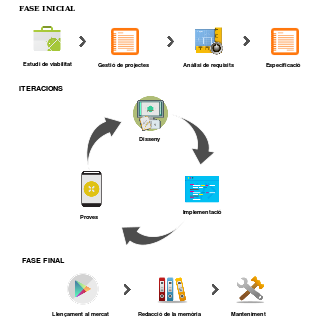
\includegraphics[scale=1]{Figures/metodologia.png}
\caption{Metodologia}
\end{figure}



\section{Eines de seguiment}

Per tal de portar un control de la feina feta s’utilitzen diferents eines de seguiment. En la part d’implementació, durant les iteracions, s’utilitza la eina Toggl. Toggl és un software disponible a la xarxa que permet portar el control del temps que dediques a una tasca en concret. Per tant, a cada historia d’usuari que es comença se li assigna una nova tasca i es fica el cronòmetre en marxa. A la figura 2.1 es pot veure
un exemple d’utilització de l’eina.\\

Una altra eina de seguiment és la preparació de les reunions amb la tutora del projecte, normalment, una reunió al final de cada iteració. A l’inici de cada sprint, com a planificació d’aquest, es redacta un informe on hi apareix l’esquema de casos dús on es pot diferenciar entre els que han sigut implementats, els que es preten implementar en l’sprint i els que queden pendents; un anàlisi de les tecnologies que s’han d’utilitzar durant la iteració (APIs, serveis externs, etc) i l’especificació dels
casos d’ús que es volen implementar en la iteració.\\

Quan s’acaba una iteració, a mode de resum, també es redacta un document
valorant la feina que s’ha fet i remarcant qualsevol aspecte important per la implementació del projecte.

\begin{figure}[!h]
\centering
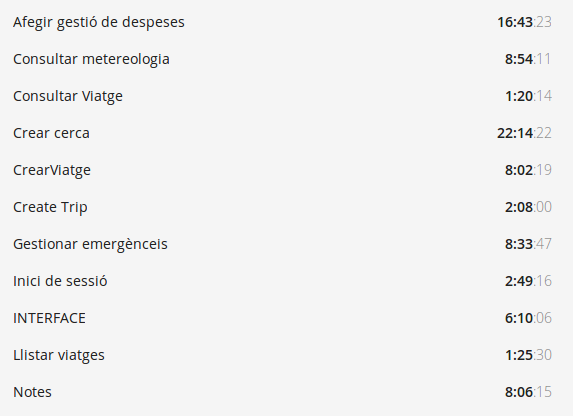
\includegraphics[scale=0.65]{Figures/toggl.jpg}
\caption{Resum de tasques a Toggl.}
\end{figure}

\section{Adequació a Enginyeria del Software}

Aquest projecte és un treball de final de grau de modalitat A, l’alumne proposa una idea i la desenvolupa. En aquest cas la idea que pretén desenvolupar aquest projecte és una aplicació mòbil de suport al viatger. En ser una aplicació mòbil el projecte necessita un bon disseny a nivell de software, cosa que requereix comptar amb un dissenyador amb coneixements prou avançats d’enginyeria del software. Aconseguir un bon disseny permetrà obtenir una aplicació sòlida, neta i molt fàcil de
mantenir.\\

Un altre punt important d’aquest projecte és que es caracteritza per utilitzar aplicacions ja existents en el mercat. Això significa que és necessari dissenyar l’aplicació de tal manera que permeti utilitzar serveis que estan disponibles al núvol.\\

A més, en el món dels serveis web hi ha avanços molt sovint i surten noves
aplicacions cada cert període de temps. És per això que aquesta aplicació vol estar preparada per tal d’assumir canvis pagant el preu més baix possible. Per tant, aquesta aplicació pretén ser dissenyada de manera que sigui molt senzill adjuntar noves funcionalitats o eliminar alguna de les existents, és a dir, pretén potenciar l’escalabilitat.

\subsection{Competències tècniques del projecte}
\begin{itemize}
\item{}CES1.1: Desenvolupar, mantenir i avaluar sistemes i serveis software complexos i/o crítics. [En profunditat]\\
És l’essència del projecte ja que es tracta de desenvolupar i mantenir un servei software d’una certa complexitat. Aquesta competència s’assoleix amb el desenvolupament complet del projecte.
\item{}CES1.2: Donar solució a problemes d’integració en funció de les estratègies, dels estàndards i de les tecnologies disponibles. [Una mica]\\
L’aplicació necessita la participació d’aplicacions externes per tal  d’aconseguir certes funcionalitats, per tant, és necessàri la integració de les dades que arriben des dels serveis exteriors.
\item{}CES1.3: Identificar, avaluar i gestionar els riscos potencials associats a la construcció de software que es poguessin presentar. [Bastant]\\
Aquest objectiu s’assoleix durant l’estudi de viabilitat del projecte ja que s’ha de preveure quins seran els possibles riscos a l’hora del desenvolupament.
\item{}CES1.5: Especificar, dissenyar, implementar i avaluar bases de dades. [Una mica]\\
Per dur a terme aquest projecte serà necessari el desenvolupament d’una ba-
se de dades, per tant, amb el disseny i desenvolupament d’aquesta s’assolirà aquesta competència.
\item{}CES1.6: Administrar bases de dades (CIS4.3) [Una mica]\\
Un cop l’aplicació estigui posada en marxa s’haurà d’administrar la base de
dades, per aquest motiu la competència no incideix en profunditat. Aquesta
competència s’assolirà un cop acabat el projecte.

\item{}CES1.7: Controlar la qualitat i dissenyar proves en la producció de software. [En profunditat]\\
En utiltizar una metodologia Agile es dona molta importància al control de
qualitat i a les proves durant el desenvolupament, aquesta competència es posarà a prova en profunditat durant el desenvolupament del producte.
\item{}CES1.9: Demostrar comprensió en la gestió i govern dels sistemes software. [En profunditat]\\
Desenvolupar una aplicació com aquesta requereix d’una bona gestió del sistema software, per aquest motiu es treballa aquesta competència en profunditat i s’assoleix havent acabat el projecte amb èxit.
\item{}CES2.1: Definir i gestionar els requisits d’un sistema software. [En profunditat]\\
Durant l’especificació de requisits es quan es treballa i s’assoleix aquesta competència, és una part bàsica del projecte i per aquest motiu es treballa en profunditat.
\item{}CES2.2: Dissenyar solucions apropiades en un o més dominis d’aplicació, utilitzant mètodes d’enginyeria del software que integrin aspectes ètics, socials, legals i econòmics. [En profunditat]\\
En el desenvolupament del projecte és necessari dissenyar solucions apropiades utilitzant mètodes d’enginyeria del software, s’assolirà aquesta competència en profunditat havent acabat el projecte amb èxit.
\end{itemize}

\subsection{Coneixements Aplicats}
Durant la meva estada a la FIB he cursat vàries assignatures amb continguts molt interessants a l’hora de desenvolupar aquest projecte. En especial, les que més s’apliquen en aquest projecte a nivell tècnic són:
\begin{itemize}
\item{}\textbf{AS:} Tots els continguts tècnics d’arquitectura de software.
\item{}\textbf{GPS:} En aquesta assignatura es va treballar la gestió de projectes, en aquest cas, la part d’Agile és la més important.
\item{}\textbf{PES:} Durant el desenvolupament del projecte d’especialitat es va fabricar una aplicació Android com la que es desenvolupa en aquest projecte. A més es van utilitzar mètodes de seguiment i metodologia que s’aplica a aquest projecte.
\item{}\textbf{ASW:} Aquesta aplicació necessita utilitzar serveis web, cosa que es va exposar en l’assignatura ASW.
\item{}\textbf{ER:} Durant l’especificació de requisists s’ha utilitzant en tot moment els coneixements adquirits cursant aquesta assignatura.
\item{}\textbf{BD:} Per tal de dissenyar la base de dades s’ha posat en pràctica part dels coneixements adquirits a l’assignatura.
\item{}\textbf{CBDE:} Per tal de dissenyar la base de dades s’ha posat en pràctica els coneixements i l’esperit crític adquirit a l’assignatura sobre les bases de dades no relacionals.

\end{itemize}

% Chapter Template

\chapter{Planificació temporal} % Main chapter title

\label{Planificacio} % Change X to a consecutive number; for referencing this chapter elsewhere, use \ref{ChapterX}

El projecte està delimitat temporalment entre el mes de febrer del 2017 i el
mes de juny del 2017. L’assignatura GEP dona el tret de sortida al TFG ja
que els lliuraments d’aquesta assignatura són parts de la memòria final del
projecte. El projecte s’inicia el dia 13 de febrer i s’acaba a finals de juny amb la presentació oral. No obstant es marca una data límit prèvia a la presentació per tal d’assegurar que el projecte tingui una certa maduresa el dia de la defensa, aquest dia és el 15 de juny.

\section{Descripció de les tasques}

S’ha dividit la feina en tres grans fases. Per cadascuna d’elles s’explica quines tasques es duen a terme i les hores de dedicació previstes.

\begin{itemize}
\item{}\textbf{Fase inicial}\\
En la fase inicial del projecte és bàsic determinar que es vol construir.
Aquesta part del desenvolupament del projecte està marcada per la gestió del mateix. Es defineix clarament quin és l’abast, el problema que es
vol solucionar, l’estat actual de l’art, la metodologia a seguir, la planificació i la gestió econòmica.\\

En aquesta fase inicial també es dur a terme l’anàlisi de requisits del sistema, aquest punt es força important ja que és bàsic definir què ha de
satisfer l’aplicació per tal de considerar-la completa.\\

El projecte segueix la metodologia àgil Scrum, per tant, la definició del
backlog determinarà les històries d’usuari que s’han d’implementar per
tal de dur a terme el projecte. Una història d’usuari és una característica o funcionalitat de la plataforma independent a la resta, i per tant, el backlog és el conjunt ordenat d’aquestes característiques o funcionalitats. Quan es defineix una història d’usuari també s’hi afegeixen els criteris d’acceptació, que són unes condicions que ha de satisfer el sistema per tal de donar la història per acabada. El criteri que es fa servir per ordenar el backlog és la importància de la pròpia història i a l’hora de la selecció de les històries a desenvolupar durant una iteració concreta es mira l’ordre però també el tamany de la història. El tamany de la història ve definit pels punts d’història.\\

Durant aquesta fase es preveu un treball diari de 3 hores.

\item{}\textbf{Iteracions}\\
Una iteració es un període de temps durant el qual s’ha de desenvolupar
un conjunt d’històries d’usuari prèviament seleccionades. És important
que es desenvolupin de manera vertical, és a dir, en acabar una iteració
s’ha de tenir software que funcioni i, a més, integrat al que s’havia desenvolupat en la iteració anterior.\\

En l’inici de cada iteració es seleccionen les històries d’usuari que es volen desenvolupar i es crea un tauler utilitzant l’eina Trello. A mesura que es van completant aquestes histories es fan proves per veure que tot funcioni i es donen per acabades. El dia que acaba la iteració es valora la feina feta i es redefineix la velocitat (punts d’historia per iteració).
Durant el desenvolupament del projecte es duran a terme 5 iteracions distribuides en les següents dates:
\begin{itemize}
\item{}Iteració 1: 29 de març - 12 d’abril
\item{}Iteració 2: 13 d’abril - 26 d’abril
\item{}Iteració 3: 27 d’abril - 10 de maig
\item{}Iteració 4: 11 de maig - 24 de maig
\item{}Iteració 5: 25 de maig - 7 de juny
\end{itemize}
Durant aquesta fase del projecte es preveu un treball de 4 hores al dia.
\item{}\textbf{Fase final}\\
En la fase final del projecte es dedicaran tots els esforços en la redacció de
la memòria del projecte i la preparació de la presentació final. A més, es
duran a terme proves de l’aplicació amb la participació d’usuaris reals.
Aquesta fase es comença el dia 8 de juny i finalitza el dia 16 de juny amb
la previsió d’un treball diari de 3 hores.

\end{itemize}

\section{Diagrama de Gantt}

Per tal de definir bé la planificació del projecte s’utilitza un diagrama de Gantt (figura 3.2) i una taula explicativa (figura 3.1).

\begin{figure}[!h]
\centering
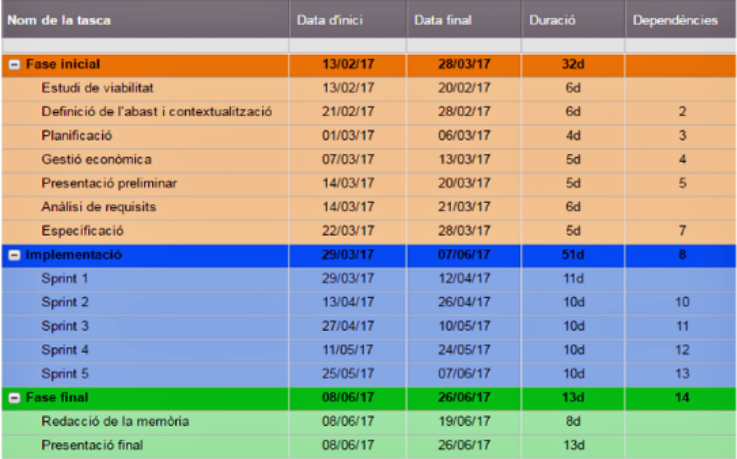
\includegraphics[scale=0.65]{Figures/planificacio.jpg}
\caption{Planificació del projecte.}
\end{figure}

\begin{figure}[!h]
\centering
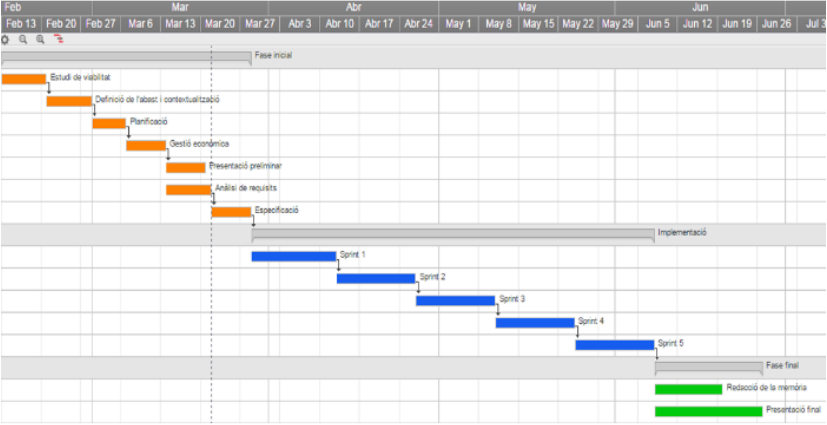
\includegraphics[scale=0.65]{Figures/Gantt.jpg}
\caption{Diagrama de Gantt.}
\end{figure}

\section{Recursos humans}

\begin{itemize}

\item{}\textbf{Cap de projecte:} Encarregat de la planificació i supervisió de les tasques a desenvolupar en un projecte així com de l’organització, coordinació i mediació de l’equip de recursos humans.
\item{}\textbf{Analista:} Estudia els problemas actuals per proposar una solución òptima i d’acord als recursos disponibles. Proporcionen les funcionalitats que tindrà el sistema mitjançant el model de casos d’ús.
\item{}\textbf{Dissenyador:} En base a la documentació proporcionada pels analistes, s’estructura i es defineix una arquitectura pel sistema que s’ha de desenvolupar. 
\item{}\textbf{Programador:} S’encarrega d’implementar el disseny proposat pels dissenyadors d’una forma eficient.
\item{}\textbf{Tester:} Prova el sistema per tal de detectar errors o recomanar modificacions, ha de redactar un informe després de cada prova efectuada.
\end{itemize}

\section{Recursos tècnics}

\newcolumntype{L}{>{\centering}m{4cm}}
\newcolumntype{M}{m{4cm}}
\newcolumntype{T}{m{12cm}}

\newcommand\tab[1][0.75cm]{\hspace*{#1}}

\begin{table}[!h]
\begin{tabular}{|M|L|M|}
\hline
\textbf{Recurs}& Tipus & Finalitat  \\ \hline
Recurs
Ordinador portàtil
Packard Bell i7, 4 GB
de Ram i windows 7
64x & Eina de desenvolupament & Desenvolupar l’aplicació i la memòria \\ \hline
Motorola Moto G amb Android 5.0 & Eina de desenvolupament &
Dur a terme les proves
durant el desenvolupament de l’aplicació \\ \hline
Android Studio v2.2.1 &
Eina de desenvolupament &
Desenvolupar l’aplicació mòbil. \\ \hline
Microsoft Office word
2007
Microsoft Office Power
Point 2007 & Eina de desenvolupament & Redacció d’informes \\ \hline
Point 2007
Adobe Photoshop 9 & Eina de desenvolupament & Edició i maquetació de
la presentació final. \\\hline
Adobe Reader XI & Eina de desenvolupament & Visualització de documents\\\hline
Correu electrònic
Gmail & Eina de comunicació & Comunicació amb la tutora del projecte\\\hline
Git & Eina de desenvolupament & Control de versions del codi font de l’aplicació \\\hline
LateX & Eina de desenvolupament & Redacció de la memòria final \\\hline
\end{tabular}
\label{}
\caption{Recursos tècnics}
\end{table}

\section{Valoració d'alternatives i pla d'acció}

Durant el desenvolupament del projecte poden sorgir desviacions de dos tipus:
\begin{itemize}

\item{}\textbf{Errors en la planificació}\\
Resulta força complicat ser precís en la planificació del projecte ja que és un equip completament nou en aquesta disciplina.\\

L’error pot venir donat per una planificació massa pessimista, en aquest
cas no hi hauria cap problema ja que durant les iteracions es podrien agafar més històries d’usuari seguint l’ordre del backlog. Acabar el projecte abans d’hora no seria perjudicial.\\

D’altra banda, l’error pot ser causat per una planificació massa optimis-
ta. En aquest cas si que és un problema ja que significa que l’equip no
pot acabar la feina a temps. Per afrontar aquesta situació s’ha reservat un
període d’una setmana abans de l’entrega final del projecte que es podria
utilitzar per acabar les històries pendents. A més, durant l’última iteració s’estudiaria l’opció de realitzar hores extra, i en el cas que no es pugui dur a terme tot el projecte es deixarien sense implementar les últimes històries del backlog ja que sempre són les menys prioritàries.\\

Tot i aquestes possibles desviacions degut a una mala planificació a cada final d’iteració i reunió amb la tutora s’evaluarà la situació i tenint en
compte les dates marcades es reafirmarà la planificació establerta o es fa-
ran les modificacions necessàries.

\item{}\textbf{Imprevistos}\\
Durant el desenvolupament del projecte poden sorgir imprevistos que
sigui quin sigui l’origen d’aquestes es solucionaran fent hores extra i prioritzant les tasques que aportin més valor al projecte.

\end{itemize}


% Chapter Template

\chapter{Gestió Econòmica} % Main chapter title

\label{GestioEconomica} % Change X to a consecutive number; for referencing this chapter elsewhere, use \ref{ChapterX}

\section{Identificació i estimació dels costos}
En aquest punt es fa una estimació dels elements que formen part del pressupost del projecte tenint en compte els recursos que s'utilitzen.

\begin{itemize}
\item{}\textbf{Recursos humans}\\
Aquest projecte el desenvolupa únicament una persona, per aquest motiu
es necessari adoptar diferents rols. A continuació es mostra una taula amb
el preu que cobra per hora cada perfil implicat en el projecte, les hores
estimades que durà a terme cada rol i el cost total.

\begin{table}[!h]
\centering
\begin{tabular}{|c|c|c|c|c|}
\hline
\textbf{Recursos} & \textbf{Rol} & \textbf{\euro/h} & \textbf{Estimació en hores} & \textbf{Total estimat} \\ \hline
& Cap de projecte & 45 \euro/h & 160 h & 7.200 \euro \\ \cline {2-5}
\multicolumn{ 1}{|l|}{} & Analista & 30 \euro/h & 45 h & 1.350 \euro \\ \cline{ 2- 5}
Pere Bergé & Dissenyador & 30 \euro/h & 70 h & 2.100 \euro \\ \cline{ 2- 5}
\multicolumn{ 1}{|l|}{} & Programador & 25 \euro/h & 104 h & 2.600 \euro \\ \cline{ 2- 5}
\multicolumn{ 1}{|l|}{} & Tester & 15 \euro/h & 30 h & 450 \euro \\ \hline
\multicolumn{ 1}{|l|}{} & & & 409 h & 13.700 \euro \\ \hline
\end{tabular}
\label{}
\caption{Estimació cost recursos humans}
\end{table}

\item{}\textbf{Software}\\
Per dur a terme aquest projecte són necessàries diverses eines de software,
la majoria d'elles gratuïtes.

\begin{table}[!h]
\centering
\begin{tabular}{|c|c|c|c|}
\hline
\textbf{Producte} & \textbf{Cost} & \textbf{Vida útil} & \textbf{Amortització total(5 mesos)} \\ \hline
Windows 7 & 0\euro & - & 0\euro \\\hline
Microssoft Office 2013 & 119\euro & 4 anys & 12,40\euro \\\hline
Android Studio 1.5.1 & 0\euro & - & 0\euro \\\hline
Mozilla Firefox & 0\euro & - & 0\euro \\\hline
Google Drive & 0\euro & - & 0\euro \\\hline
Trello & 0\euro & - & 0\euro \\\hline
SmartSheet & 0\euro & - & 0\euro \\\hline
Adobe Photoshop & 12,09\euro/mes & 5 mesos & 60,45\euro \\\hline
Adobe Reader IX & 0\euro & - & 0\euro \\\hline
Github & 0\euro & - & 0\euro \\\hline
\textbf{Total} & & & 72,85\euro \\\hline
\end{tabular}
\label{}
\caption{Estimació cost recursos software}
\end{table}

\clearpage

\item{}\textbf{Hardware}

\begin{table}[!h]
\centering
\begin{tabular}{|c|c|c|c|}
\hline
\textbf{Producte} & \textbf{Cost} & \textbf{Vida útil} & \textbf{Amortització total(5 mesos)} \\ \hline
Ordinador portàtil & 600\euro/mes & 5 anys & 50\euro \\\hline
Smartphone & 190\euro & 3 anys & 26,39\euro \\\hline
\textbf{Total} & & & 76,39\euro \\\hline
\end{tabular}
\label{}
\caption{Estimació cost recursos hardware}
\end{table}

\item{}\textbf{Despeses generals}\\
En aquest apartat es tenen en compte les despeses associades a la realització del projecte com poden ser la energia elèctrica consumida o l'accés a internet.

\begin{table}[!h]
\centering
\begin{tabular}{|c|c|c|c|}
\hline
\textbf{Producte} & \textbf{Cost} & \textbf{Periode} & \textbf{Total estimat} \\ \hline
Energia elèctrica & 0,15\euro/kWh*0,15kW & 409 h & 9,20\euro \\\hline
Llicència desenvolupador \textit{Android} & 19\euro & Indefinit & 19\euro \\\hline
Accés a internet & 25\euro & 5 mesos & 125\euro \\\hline
\textbf{Total} & & & 153,2\euro \\\hline
\end{tabular}
\label{}
\caption{Estimació cost despeses generals}
\end{table}

\item{}\textbf{Costos directes}\\
En aquest apartat s'agrupen tots els costos directes que suposa el desenvolupament d'aquest projecte.

\begin{table}[!h]
\centering
\begin{tabular}{|l|c|}
\hline
\textbf{Concepte} & \textbf{Cost} \\\hline
Recursos humans & 13.700\euro \\\hline
Software & 73\euro \\\hline
Hardware & 77\euro \\\hline
\textbf{Total} & 13.850\euro \\\hline
\end{tabular}
\label{}
\caption{Estimació costos directes}
\end{table}

\item{}\textbf{Costos d'imprevistos}\\
L'únic cost imprevist que podria sorgir és una fallada en l'ordinador o l'smartphone que s'utilitzen pel desenvolupament del projecte. En cas de fallada s'hauria d'afegir el cost de reparació, aproximadament uns 150 \euro en cas de l'ordinador i 60 \euro en cas del dispositiu Android. Durant el transcurs de la reparació s'utilitzaria un segon aparell per tal de no bloquejar el desenvolupament del projecte. La probabilitat d'error d'ambdós aparells és d'un 15 \%.

\begin{table}[!h]
\centering
\begin{tabular}{|l|c|c|c|}
\hline
\textbf{Producte} & \textbf{Cost Reparació} & \textbf{Probabilitat d'error} & \textbf{Total estimat} \\ \hline
Ordinador & 150\euro & 15\% & 22,5\euro \\\hline
Dispositiu \textit{Android} & 60\euro & 15\% & 9\euro \\\hline
\textbf{Total} & - & - & 31,5\euro \\\hline
\end{tabular}
\label{}
\caption{Estimació cost d'imprevistos}
\end{table}

\clearpage

\item{}\textbf{Cost total del projecte}
\begin{table}[!h]
\centering
\begin{tabular}{|l|c|}
\hline
\textbf{Concepte} & \textbf{Cost} \\\hline
Costos directes & 13.850\euro \\\hline
Despeses generals & 153,2\euro \\\hline
Cost d'imprevistos & 31,5\euro \\\hline
Contingències (5\%) & 701,7\euro \\\hline
\textbf{Total} & 14.740\euro \\\hline
\end{tabular}
\label{}
\caption{Estimació cost total del projecte}
\end{table}

\end{itemize}

\section{Control de gestió}
Per al control de gestió es planteja omplir unes taules amb les hores reals que dur a terme cadascun dels rols. Cada dia s'han d'actualitzar i d'aquesta manera es pot portar un control i veure possibles desviacions en la planificació.

\begin{table}[!h]
\centering
\begin{tabular}{|c|c|c|c|c|c|}
\hline
\textbf{Dia} & \textbf{Cap de Projecte} & \textbf{Analista} & \textbf{Dissenyador} & \textbf{Programador} & \textbf{Tester} \\ \hline
28/02/17 & 3h & - & - & - & - \\\hline
\end{tabular}
\label{}
\caption{Control d'hores reals}
\end{table}

Al final del projecte es farà un recompte de les hores reals i es compararan amb les estimades, d'aquesta manera es podrà analitzar la precisió de l'estimació. Les dades es presentaran en una taula com la que es mostra a continuació.

\begin{table}[!h]
\centering
\begin{tabular}{|c|c|c|c|c|c|}
\hline
\textbf{Rol} & \textbf{Hores estimades} & \textbf{Cost estimat} & \textbf{Hores reals} & \textbf{Cost real} \\ \hline
Cap de projecte & 160h & 7.200\euro & 170h & 7.650\euro \\\hline
Analista & 45h & 1.350\euro & 65h & 1.900\euro \\\hline
\end{tabular}
\label{}
\caption{Comparació cost estimat i cost real}
\end{table}


% Chapter Template

\chapter{Anàlisi Inicial} % Main chapter title

\label{AnalisiInicial} % Change X to a consecutive number; for referencing this chapter elsewhere, use \ref{ChapterX}

En aquest apartat es descriu el procés realitzat durant la primera part del treball amb l’estudi de viabilitat, l’anàlisi de riscs, les funcions que s’han ideat per al sistema i una valoració i justificació de les tecnologies disponibles per a dur a terme el projecte.

\section{Estudi de viabilitat}
Per tal d’estudiar la viabilitat del projecte es necessari conèixer quines persones poden interaccionar amb el sistema i els termes legals associats per tal que la posada en funcionament del sistema compleixi amb la llei establerta.

\subsection{Anàlisi de les parts interessades}
En el cas concret de l’aplicació a desenvolupar es considera que només existeix
un rol en la interacció. L’usuari pren el rol de viatger, que és qui interactua
amb l’aplicació a l’hora d’introduir i consultar dades. Cal dir però que també
existeixen dos tipus d’actors indirectes:

\begin{itemize}
\item{}Persona de contacte: és a qui es truca en cas de que l’usuari tingui alguna emergència. No interactua amb l’aplicació però en forma part indirectament.
\item{}Viatger no usuari: són els companys de viatge de l’usuari en cas de que els tingui, no interactuen amb l’aplicació però se’ls envia avisos en cas de tenir deutes pendents amb l’usuari. A més, se’ls pot etiquetar en notes.
\end{itemize}

\subsection{Limitacions legals implicades}
En la gestió i emmagatzematge de dades sensibles de l’usuari s’ha tingut en
compte que, segons la Llei Orgànica de Protecció de Dades (LOPD) , les dades externes que guarda el projecte són dades de nivell baix de seguretat. La LOPD pretén garantir el dret a controlar què es fa amb les nostres dades, saber qui té informació sobre nosaltres, quina informació té, d’on l’ha obtingut, per a quina finalitat té les dades i si té intenció de facilitar-les a un tercer.\\

Per complir amb la llei, abans de que el sistema es posi en funcionament caldrà realitzar una sèrie d’accions:
\begin{itemize}
\item{}Inscripció de fitxers: s’ha d’informar a l’Agència Espanyola de Protecció de Dades (AEPD) de l’existència dels fitxers que es van a utiltzar. La AEPD comprovarà si es compleixen els requisits i els incriurà.
\item{}Elaboració document de seguretat: s’ha d’elaborar un document on es
descriran les mesures de seguretat aplicades a cada fitxer. Ha de ser respectat obligatoriament per tot el personal i s’ha de mantenir actualitzat, afegint les modificacions pertinents en cas que el nivell de protecció de dades hagi de canviar.
\item{}Deure d’informació: s’ha d’informar a l’usuari del tractament que se’n farà i dels destinataris a qui es farà arribar aquesta informació.
\item{}Seguretat de les dades: s’ha de garantir que les dades no es perden, per aquest motiu, serà necessari crear còpies de seguretat.

\end{itemize}

\section{Anàlisi de riscs}

En el capítol 2 hem vist l’apartat d’Obstacles on s’identifiquen una sèrie de
riscs que té el projecte. En aquest punt es mostra estratègies per tal d’evitar-los
i un pla per afrontar el problema provocat per si les estratègies anteriors fallen.

\subsection{Estratègies de prevenció}
Tenint en compte els riscs que podrien sofrir el sistema un cop en funcionament, és important fer una previsió de les accions que es duen a terme per tal d’evitar que els riscs es materialitzin en problemes reals.
\begin{itemize}
\item{}Nivell baix de bateria.\\
L’usuari és l’encarregat d’activar les notificacions per nivell de bateria
baix en el sistema operatiu del seu mòbil.
\item{}Connexió a internet a l’estranger.\\
Cada cop és més corrent tenir contractades dades fora del país de residèn-
cia, tot i així, és l’usuari qui ha de buscar connexió a internet a través de xarxes d’internet gratuïtes o de pagament.
\item{}Caiguda del servei web.\\
Es buscaran serveis de qualitat amb una tassa de caigudes molt baixa.
\item{}Caiguda de la base de dades.\\
Es buscarà un proveïdor de base de dades al núvol que ofereixi un servei
de qualitat i amb una tassa de caigudes molt baixa. A l’hora de efectuar el
manteniment, es faran proves prèviament per tal de que quan s’apliquin
els canvis no hi hagi problemes.
\item{}Canvis en la legislació.\\
Aquest és un risc que no es pot evitar.
\item{}Desconfiguració de l’aplicació.\\
A causa de canvis en el sistema operatiu del dispositiu mòbil o actualit-
zacions de l’aplicació aquesta pot deixar de funcionar correctament.
\item{}Canvis en la resposta del servei web.\\
Es buscaran serveis web estables i amb una certa maduresa.

\end{itemize}

\subsection{Plans per afrontar obstacles}

En el cas que sigui impossible evitar l’aparició de problemes, s’ha elaborat un pla d’actuació per afrontar aquests possibles obstacles i així minimitzar el problema un cop ha aparegut.

\begin{itemize}

\item{}Nivell baix de bateria.\\
Es tasca de l’usuari tenir bateria al dispositiu mòbil, d’altra manera l’aplicació no pot funcinar.
\item{}Connexió a internet a l’estranger.\\
Es tasca de l’usuari obtenir connexió a internet a l’estranger. En cas de no tenir connexió, l’aplicació suggerirà a l’usuari a través d’un avís que es connecti a una xarxa wifi.
\item{}Caiguda del servei web.\\
En cas que un usuari accedeixi a un servei web no disponible, es bloquejarà la funcionalitat que l’utilitza i es notificarà a l’equip de manteniment.
\item{}Caiguda de la base de dades.\\
Si en el moment d’emmagatzemar o consultar dades la base dades no està
operativa, es mostrarà un missatge d’error alertant a l’usuari. En aquest
missatge s’inclourà informació per notificar l’error i tractar de solucionar-lo ràidament.
\item{}Canvis en la legislació.\\
Estudiar l’impacte que té sobre el sistema i fer les modificacions corres-
ponents per a complir amb la nova llei establerta.
\item{}Desconfiguració de l’aplicació.\\
L’aplicació inclourà una secció d’ajuda on l’usuari pot trobar solució a
problemes freqüents. Si el problema persisteix, l’usuari haurà de posar-se
en contacte amb el servei tècnic.
\item{}Canvis en la resposta del servei web.\\
Si l’aplicació detecta problems a l’hora de llegir la informació aquesta bloquejarà la funcionalitat que afecta i notificarà a l’equip de manteniment.
\end{itemize}

\section{Visió global de les funcionalitats del sistema}
Finalment, es llisten les funcionalitats que oferirà el sistema un cop completat el seu desenvolupament.

\begin{itemize}

\item{}\textbf{Gestió de despeses del viatge}\\
La funcionalitat de gestió de despeses es basa en portar un control de les
despeses del viatge. Es divideix en dos parts: el control de les despeses
total i el control de deutes entre l’usuari i els altres viatgers. El control de despeses total es basa en anar afegint les despeses adjuntant-hi un motiu i una localització. D’altra banda, el control de deutes entre els viatges es basa en que si l’usuari paga alguna cosa a un altre viatger s’anota el deute i se li envia un correu electrònic al deutor.
\item{}\textbf{Gestió de cerques de llocs d’interès i com arribar-hi}\\
La funcionalitat de cerques de llocs d’interès es basa en que l’usuari pot
llençar qualsevol cerca sobre el mapa i l’aplicació respondrà mostrant-li
un conjunt de punts representats en el mapa ordenats segons les seves
preferències a l’hora de viatjar.
\item{}\textbf{Gestió d’emergències}\\
La funcionaltiat de gestió d’emergències té diverses parts. La primera és
l’opció de buscar l’hospital o farmàcia més propers mostrant la ruta sobre
el mapa. També ofereix informació dels telèfons d’emergència més importants del país on es troba l’usuari i, per últim, ofereix l’opció de trucar
fàcilment al telèfon de contacte que ha introduït l’usuari a l’inici del viatge.
\item{}\textbf{Previsió metereològica}\\
La funcionalitat de previsions metereològiques ofereix la previsió de la
setmana del lloc on es viatja amb la possibilitat d’afegir noves localitzacions per tal de portar un control de la metereologia de diferents llocs.
\item{}\textbf{Gestió de notes}\\
La funcionalitat de gestió de notes pretén ser un suport a l’hora de guardar curiositats, anèctodes o fets rellevants que succeeixen durant el viatge.
A més, l’aplicació dona l’opció de compartir la nota amb els participants del viatge.

\end{itemize}

\section{Anàlisi de les tecnologies candidates}

\subsection{Plataforma}
En ser una aplicació orientada al món viatger, es considera que la tecnologia més adequada és una que permeti mobilitat. A continuació es mostren els avantatges i inconvenients de la tecnologia candidata, el telèfon mòbil.\\
\textbf{Avantatges:}
\begin{itemize}
\item{}Ofereix mobilitat a l’usuari, pot ser utilitzat en qualsevol lloc.
\item{}Permet l’accés a internet.
\item{}Permet fer trucades telefòniques.
\item{}Gairebé la totalitat de la població disposa d’accés a aquesta tecnologia.
\item{}Molt fàcil d’utilitzar i instal·lar.
\end{itemize}

\textbf{Inconvenients:}
\begin{itemize}
\item{}Necessita connexió permanent.
\item{}El tamany de la pantalla és limitat.
\item{}Introduir dades és incomode.
\item{}Dependència de la bateria.
\end{itemize}

Per aquesta aplicació concerta, clarament pesen més els avantatges que els
inconvenients. És dona molta importància al fet que el dispositiu mòbil
està sempre aprop de l’usuari i aquest està molt acostumat a consultar
informació o rebre notificacions a aquest tipus de dispositiu. Per tant, no
hi ha dubte a l’hora de desenvolupar l’aplicació per a un dispositiu mòbil.

\subsection{Serveis externs}

En aquest apartat s’analitzen diferents alternatives a l’hora de seleccionar
quins serveis externs són els més adients.
\begin{itemize}
\item[]\textbf{Serveis de localització}
\begin{itemize}
\item{}\textbf{Google Maps}\\
Google Maps és l’aplicació més desenvolupada del sector i la que
ofereix més serveis com:
\begin{itemize}
\item{}Conversió de coordenades geogràfiques a direccions.
\item{}Dades d’elevació.
\item{}Rutes de navegació GPS.
\item{}Localització geogràfica.
\item{}Càlcul de temps de viatge i distància entre diverses destinacions.
\item{}Càlcul de les indicacions entre diverses destinacions.
\item{}Informació sobre els llocs.
\end{itemize}
\item{}\textbf{Foursquare}
\begin{itemize}
\item{}Cerca de llocs d’interés en una àrea concreta.
\item{}Conexió amb usuaris de l’aplicació.
\item{}Control d’accés als punts.

Aquesta aplicació retorna les dades en format JSON amb molts
paràmetres que donen informació sobre el punt d’interés seleccionat. Entre aquests paràmetres n’hi ha un que és molt interessant
ja que ens revela el nivell de preu de l’establiment.
\end{itemize}
Un cop fet l’anàlisi s’ha decidit que s’utilitzarà Foursquare per tal de
fer les cerques de llocs d’interés, ja que la resposta en format JSON
és perfecta per tal de obtenir la informació i poder filtrarla, i Google
Maps per tal de contruir les rutes i per representar les dades al mapa
ja que és l’aplicació que ofereix el servei de manera més intuïtiva i
gairebé la totalitat dels usuaris estan habituats a utilitzar-la.

\end{itemize}

\item[]\textbf{Serveis de metereologia}
\begin{itemize}
\item{}\textbf{OpenWeatherMap}\\
OpenWeatherMap ofereix gratuitament accés a la metereologia del
moment, a la previsió fins a 5 dies, a més també ofereix informació
sobre el mapa. Les ciutats poden ser identificades per nom, per id o
per coordenades geogràfiques. A més, ofereix serveis com:
\begin{itemize}
\item{}Metereologia actual per un lloc concret.
\item{}Previsió per 5 dies amb actualitzacions cada 3 hores.
\item{}Mapes de precipitació, pressió, núvols i temperatura.
\end{itemize}
\item{}\textbf{DarkSky}\\
DarkSky ofereix les primeres 1000 crides del dia gratuitament i ofereix informació sobre el clima a una setmana vista. Les següents crides del dia es paguen a \$0.0001 la crida. Ofereix la possibilitat d’obtenir la informació en molts idiomes inclosos tots els que vol oferir
l’aplicació. Els serveis que ofereix són:
\begin{itemize}
\item{}Metereologia actual i previsió per una setmana.
\item{}Dades històriques.
\end{itemize}

Després d’analitzar el funcionament i la documentació d’ambdues
API es decideix utilitzar el servei d’OpenWeatherMap ja que la documentació és de més qualitat i ofereix grans facilitats en la connexió.

\end{itemize}

\item[]\textbf{Serveis telèfons d'emergència}
\begin{itemize}
\item{}\textbf{Emergency Number}\\
Aquesta API ens ofereix com a resposta informació de telèfons d’emergència de diferents tipus del país que li indiquem. L’únic problema que hi ha es que el país s’ha d’indicar per codi. Per tal de transformar el nom del país en el codi pertinent s’utilitzat un altre servei web.\\

El servei analitzat és un servei molt complert que té informació de
garibé tots els racons del món, per aquest motiu és l’el·legit a l’hora
d’aconseguir els telèfons d’emergència del païs que sigui necessari.

\end{itemize}
\end{itemize}

\section{Conclusions de l'anàlisi inicial}

Tenint un coneixement més ampli del sector i considerant com s’ha plantejat
el projecte es considera que es pot tirar endavant amb garanties d’èxit tot i
tenir en compte els possibles aspectes negatius que repercuteixen el projecte
(accessibilitat a les dades, llei, etc).


% Chapter Template

\chapter{Requisits} % Main chapter title

\label{Requisits} % Change X to a consecutive number; for referencing this chapter elsewhere, use \ref{ChapterX}

\section{Propietats i hipòtesis sobre el domini}

Per a poder desenvolupar aquest projecte, s’ha considerat necessari definir una sèrie d’expectatives sobre l’ús del sistema.
\begin{itemize}
\item{}\textbf{Connexió a internet}\\
L’usuari té connexió a internet en tot moment ja que es necessita a l’hora
de guardar i consultar dades, i a l’hora d’accedir a serveis web.
\item{}\textbf{Ús del sistema}\\
Els usuaris utilitzaran el sistema d’acord amb la finalitat per al qual ha
sigut creat sense fer-ne un mal us o emprenen accions malicioses que puguin trencar la integritat del sistema. Tot i així, s’implementaran mitjants de seguretat per protegir l’aplicació en aquest aspecte.
\item{}\textbf{Obtenció de dades correctes}\\
 Les dades que s’obtenen de serveis web són
correctes i actualitzades.

\end{itemize}

\section{Restriccions}
\begin{itemize}
\item[]\textbf{Restricció de la solució}
\begin{itemize}
\item{}Descripció: L’aplicació serà desenvolupada com a aplicació mòbil Android.
\item{}Justificació: Els dispositius mòbils estan sempre aprop de l’usuari i
disponibles per al seu ús, a més, en els últims anys s’ha extés l’ús
d’internet al mòbil. Pel que fa al sistema operatiu, degut a la limitació temporal del treball i a que té una quota de mercat molt gran a
Espanya s’ha optat per la implementació en Android, encara que no
es descarten altres sistemes operatius en un futur.
\end{itemize}
\item[]\textbf{Restricció temporal}
\begin{itemize}
\item{}Descripció: El sistema ha d’estar acabat a meitats de juny de 2017.
\item{}Justificació: S’estableix una data límit per presentar el projecte.
\end{itemize}
\item[]\textbf{Restricció econòmica}
\begin{itemize}
\item{}Descripció: El desenvolupament del projecte es durà a terme sense
cap cost econòmic.
\item{}Justificació: Com que no es disposa de cap inversió econòmica i el
projecte es desenvolupa en un entorn acadèmic les eines i serveis uti-
litzats suposaran un cost molt baix.
\end{itemize}
\end{itemize}

\section{Diagrama de casos d'ús}
En la figura 5.1 es mostra el diagrama de casos d’ús del sistema sense tenir en compte la gestió d'usuaris.

\begin{figure}[!h]
\centering
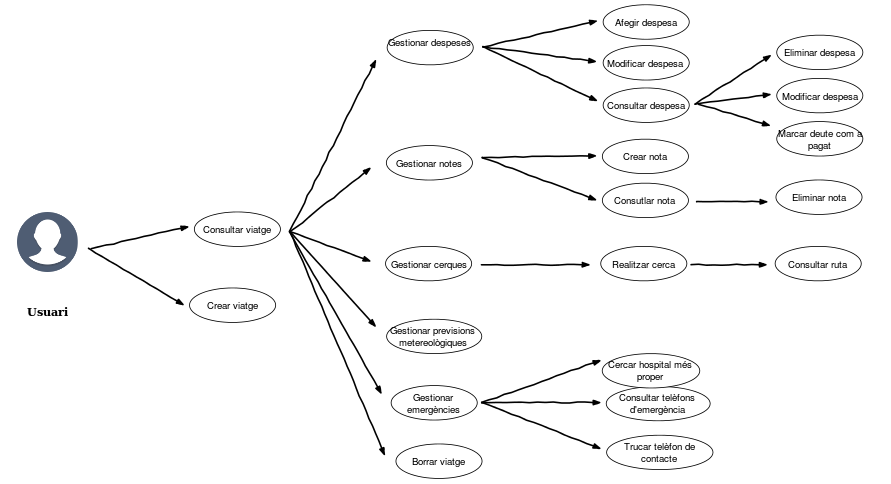
\includegraphics[scale=0.65]{Figures/casosUs.png}
\caption{Diagrama de casos d'ús}
\end{figure}

\section{Casos dús}

\newcolumntype{L}{>{\centering}m{0.75cm}}
\newcolumntype{M}{m{9cm}}
\newcolumntype{T}{m{12cm}}



\newcolumntype{L}{>{\centering}m{0.75cm}}
\newcolumntype{M}{m{9cm}}
\newcolumntype{T}{m{12cm}}



\begin{table}[!h]
\centering
\begin{tabular}{|l|L|l|}
\hline
\textbf{Cas d'ús }& \#1 &  Registrar-se al sistema  \\ \hline
\textbf{Actor principal} & \multicolumn{ 2}{l|}{Usuari} \\ \hline
\textbf{Precondició} & \multicolumn{ 2}{M|}{L'usuari té l'aplicació instal·lada al seu dispositiu.} \\ \hline
\textbf{Trigger} & \multicolumn{ 2}{M|}{L'usuari es vol registrar al sistema.} \\ \hline
\multicolumn{ 3}{|T|}{\textbf{Escenari principal d’èxit}} \\ \hline
\multicolumn{ 3}{|T|}{1. L’usuari selecciona el botó de registrar-se utilitzant el seu compte de Google.}\\
\multicolumn{ 3}{|T|}{2. El sistema redirigeix el nou registre a Google.
}\\
\multicolumn{ 3}{|T|}{3. L’usuari introdueix el seu correu electrònic i la seva contrassenya.
}\\
\multicolumn{ 3}{|T|}{4. Google valida les dades.
}\\
\multicolumn{ 3}{|T|}{5. L’usuari accepta donar permisos a l’aplicació per obtenir les dades del seu perfil.}\\
\multicolumn{ 3}{|T|}{6. El sistema registra l’usuari i inicia sessió automàticament.}\\
\hline
\multicolumn{ 3}{|T|}{\textbf{Extensions}} \\ \hline
\multicolumn{ 3}{|T|}{4.a El sistema detecta algun error en els camps introduïts.
} \\
\multicolumn{ 3}{|T|}{\tab4.a.1 El sistema notifica a l’usuari de l’error.
} \\
\multicolumn{ 3}{|T|}{\tab4.a.2 Es torna al pas 3.
} \\
\multicolumn{ 3}{|T|}{5.a L’usuari no dona permisos a l’aplicació per obtenir les dades del seu perfil.} \\
\multicolumn{ 3}{|T|}{\tab5.a.1 El sistema torna al pas 1.
} \\\hline
\end{tabular}
\label{}
\caption{Cas d'ús \textit{Registrar-se al sistema}}
\end{table}

\begin{table}[!h]
\centering
\begin{tabular}{|l|L|l|}
\hline
\textbf{Cas d'ús }& \#2 &  Iniciar sessió al sistema  \\ \hline
\textbf{Actor principal} & \multicolumn{ 2}{l|}{Usuari} \\ \hline
\textbf{Precondició} & \multicolumn{ 2}{M|}{L’usuari està registrat al sistema.} \\ \hline
\textbf{Trigger} & \multicolumn{ 2}{M|}{L’usuari vol iniciar sessió al sistema.} \\ \hline
\multicolumn{ 3}{|T|}{\textbf{Escenari principal d’èxit}} \\ \hline
\multicolumn{ 3}{|T|}{1. L’usuari introdueix el seu correu electrònic i contrasenya, i indica al sistema que vol identificar-se.}\\
\multicolumn{ 3}{|T|}{2. El sistema valida les dades, identifica l’usuari i redirigeix a l’usuari a la pantalla de viatge actual.
}\\
\hline
\multicolumn{ 3}{|T|}{\textbf{Extensions}} \\ \hline
\multicolumn{ 3}{|T|}{2.a El sistema detecta algun error en els camps introduïts.
} \\
\multicolumn{ 3}{|T|}{\tab2.a.1 El sistema notifica a l’usuari que hi ha dades incorrectes.
} \\
\multicolumn{ 3}{|T|}{\tab2.a.2 Es torna al pas 1.
} \\
\multicolumn{ 3}{|T|}{3.a L’usuari no té cap viatge actiu.
} \\
\multicolumn{ 3}{|T|}{\tab3.a.1 El sistema redirigeix l’usuari a la pantalla de llista de viatges realitzats.
} \\\hline
\end{tabular}
\label{}
\caption{Cas d'ús \textit{Iniciar sessió al sistema}}
\end{table}

\begin{table}[!h]
\centering
\begin{tabular}{|l|L|l|}
\hline
\textbf{Cas d'ús }& \#3 & Tancar sessió al sistema   \\ \hline
\textbf{Actor principal} & \multicolumn{ 2}{l|}{Usuari} \\ \hline
\textbf{Precondició} & \multicolumn{ 2}{M|}{L’usuari ha iniciat sessió al sistema.} \\ \hline
\textbf{Trigger} & \multicolumn{ 2}{M|}{L’usuari vol tancar la sessió al sistema.} \\ \hline
\multicolumn{ 3}{|T|}{\textbf{Escenari principal d’èxit}} \\ \hline
\multicolumn{ 3}{|T|}{1. L’usuari indica al sistema que vol tancar sessió.
}\\
\multicolumn{ 3}{|T|}{2. El sistema es desvincula de les dades de l’usuari actual i redirigeix l’aplicació a la pantalla d’iniciar sessió.}\\\hline
\end{tabular}
\label{}
\caption{Cas d'ús \textit{Tancar sessió al sistema}}
\end{table}

\clearpage

\begin{table}[!h]
\centering
\begin{tabular}{|l|L|l|}
\hline
\textbf{Cas d'ús }& \#4 & Crear viatge  \\ \hline
\textbf{Actor principal} & \multicolumn{ 2}{l|}{Usuari} \\ \hline
\textbf{Precondició} & \multicolumn{ 2}{M|}{L’usuari ha iniciat sessió al sistema.} \\ \hline
\textbf{Trigger} & \multicolumn{ 2}{M|}{L’usuari vol iniciar un nou viatge.} \\ \hline
\multicolumn{ 3}{|T|}{\textbf{Escenari principal d’èxit}} \\ \hline
\multicolumn{ 3}{|T|}{1. L’usuari indica que vol iniciar un nou viatge.
}\\
\multicolumn{ 3}{|T|}{2. El sistema redirecciona l’usuari a la pàgina de creació de viatge.
}\\
\multicolumn{ 3}{|T|}{3. L’usuari introdueix el nom del viatge,el destí, la data d’inici i la data final, el nom i correu electrònic de tots els viatgers que formaran part del viatge i indica que vol iniciar el viatge.
}\\
\multicolumn{ 3}{|T|}{4. El sistema valida les dades i presenta a l’usuari el formulari de preferències.
}\\
\multicolumn{ 3}{|T|}{5. L’usuari respon el formulari i indica que ja ha acabat.}\\
\multicolumn{ 3}{|T|}{6. El sistema guarda el resultat del formulari i presenta a l'usuari el formulari per a que introdueixi les dades del contacte d'emergència.}\\
\multicolumn{ 3}{|T|}{7. L'usuari introdueix les dades i indica que ja ha acabat.}\\
\multicolumn{ 3}{|T|}{8. El sistema guarda el resultat, crea el viatge amb les dades introduïdes i redirigeix l'usuari a la pantalla principal del viatge.}\\
\hline
\multicolumn{ 3}{|T|}{\textbf{Extensions}} \\ \hline
\multicolumn{ 3}{|T|}{4.a El sistema detecta errors en les dades introduïdes.
} \\
\multicolumn{ 3}{|T|}{\tab4.a.1 El sistema notifica a l’usuari que hi ha dades incorrectes.} \\
\multicolumn{ 3}{|T|}{\tab4.a.2 Es torna al pas 2.} \\
\multicolumn{ 3}{|T|}{6.a El sistema detecta que no s’ha completat el formulari.
} \\
\multicolumn{ 3}{|T|}{\tab6.a.1 El sistema notifica a l’usuari que hi ha camps incomplets.} \\
\multicolumn{ 3}{|T|}{\tab6.a.2 Es torna al pas 5.} \\\hline
\end{tabular}
\label{}
\caption{Cas d'ús \textit{Crear viatge}}
\end{table}

\begin{table}[!h]
\centering
\begin{tabular}{|l|L|l|}
\hline
\textbf{Cas d'ús }& \#5 &  Consultar llista de viatges \\ \hline
\textbf{Actor principal} & \multicolumn{ 2}{l|}{Usuari} \\ \hline
\textbf{Precondició} & \multicolumn{ 2}{M|}{L’usuari ha iniciat sessió al sistema.} \\ \hline
\textbf{Trigger} & \multicolumn{ 2}{M|}{L’usuari vol consultar viatges o ha iniciat sessió i no té cap viatge en curs.} \\ \hline
\multicolumn{ 3}{|T|}{\textbf{Escenari principal d’èxit}} \\ \hline
\multicolumn{ 3}{|T|}{1. L’usuari indica que vol consultar els seus viatges.}\\
\multicolumn{ 3}{|T|}{2. El sistema redirigeix l’usuari a la pantalla de llista de viatges.}\\\hline
\end{tabular}
\label{}
\caption{Cas d'ús \textit{Consultar llista de viatges}}
\end{table}

\begin{table}[!h]
\centering
\begin{tabular}{|l|L|l|}
\hline
\textbf{Cas d'ús }& \#6 &  Consultar informació general del viatge\\ \hline
\textbf{Actor principal} & \multicolumn{ 2}{l|}{Usuari} \\ \hline
\textbf{Precondició} & \multicolumn{ 2}{M|}{L’usuari ha creat almenys un viatge.} \\ \hline
\textbf{Trigger} & \multicolumn{ 2}{M|}{L’usuari vol consultar la informació general d'un viatge.} \\ \hline
\multicolumn{ 3}{|T|}{\textbf{Escenari principal d’èxit}} \\ \hline
\multicolumn{ 3}{|T|}{1. L’usuari indica que vol consultar la informació general d'un viatge.}\\
\multicolumn{ 3}{|T|}{2. El sistema redirigeix l’usuari a la pantalla de consultar informació general del viatge seleccionat.}\\\hline
\end{tabular}
\label{}
\caption{Cas d'ús \textit{Consultar informació general del viatge}}
\end{table}

\begin{table}[!h]
\centering
\begin{tabular}{|l|L|l|}
\hline
\textbf{Cas d'ús }& \#7 & Consultar despeses   \\ \hline
\textbf{Actor principal} & \multicolumn{ 2}{l|}{Usuari} \\ \hline
\textbf{Precondició} & \multicolumn{ 2}{M|}{L’usuari ha accedit a un viatge i ha iniciat sessió.} \\ \hline
\textbf{Trigger} & \multicolumn{ 2}{M|}{L’usuari vol accedir a la funcionalitat gestió de despeses.} \\ \hline
\multicolumn{ 3}{|T|}{\textbf{Escenari principal d’èxit}} \\ \hline
\multicolumn{ 3}{|T|}{1. L’usuari indica que vol accedir a la funcionalitat gestió de despeses.}\\
\multicolumn{ 3}{|T|}{2. El sistema el redirigeix a la pantalla d’estadístiques de despeses on es mostra la despesa total, la mitjana \euro/dia i la llista de les despeses.}\\
\hline
\end{tabular}
\label{}
\caption{Cas d'ús \textit{Consultar despeses}}
\end{table}


\begin{table}[!h]
\centering
\begin{tabular}{|l|L|l|}
\hline
\textbf{Cas d'ús }& \#8 & Afegir nova despesa  \\ \hline
\textbf{Actor principal} & \multicolumn{ 2}{l|}{Usuari} \\ \hline
\textbf{Precondició} & \multicolumn{ 2}{M|}{L’usuari ha accedit a la funcionaltiat gestió de despeses compartides.} \\ \hline
\textbf{Trigger} & \multicolumn{ 2}{M|}{L’usuari vol afegir una nova despesa.} \\ \hline
\multicolumn{ 3}{|T|}{\textbf{Escenari principal d’èxit}} \\ \hline
\multicolumn{ 3}{|T|}{1. L’usuari indica que vol afegir una nova despesa.}\\
\multicolumn{ 3}{|T|}{2. El sistema redirigeix l’usuari a la pantalla de nova despesa.}\\
\multicolumn{ 3}{|T|}{3. L’usuari introdueix la quantitat que paga.}\\
\multicolumn{ 3}{|T|}{4. El sistema guarda les dades, crea la nova despesa, actualitza les estadístiques.}\\
\hline
\multicolumn{ 3}{|T|}{\textbf{Extensions}} \\ \hline
\multicolumn{ 3}{|T|}{3.a L’usuari notifica que vol crear un deute.} \\
\multicolumn{ 3}{|T|}{\tab3.a.1  L’usuari indica el participant deutor i la quantitat.
} \\
\multicolumn{ 3}{|T|}{\tab3.a.2  El sistema guarda els deutes i envia un avís als deutors.} \\
\multicolumn{ 3}{|T|}{4.a El sistema detecta dades incompatibles introduïdes per l’usuari.} \\
\multicolumn{ 3}{|T|}{\tab4.a.1 El sistema notifica a l’usuari que s’han detectat dades incompatibles.} \\
\multicolumn{ 3}{|T|}{\tab4.a.2 Es torna al pas 2.} \\\hline
\end{tabular}
\label{}
\caption{Cas d'ús \textit{Afegir nova despesa}}
\end{table}

\clearpage

\begin{table}[!h]
\centering
\begin{tabular}{|l|L|l|}
\hline
\textbf{Cas d'ús }& \#9 & Eliminar despesa   \\ \hline
\textbf{Actor principal} & \multicolumn{ 2}{l|}{Usuari} \\ \hline
\textbf{Precondició} & \multicolumn{ 2}{M|}{L’usuari ha accedit a la funcionalitat gestió de despeses compartides i ha creat almenys una despesa.} \\ \hline
\textbf{Trigger} & \multicolumn{ 2}{M|}{L’usuari vol eliminar una despesa.} \\ \hline
\multicolumn{ 3}{|T|}{\textbf{Escenari principal d’èxit}} \\ \hline
\multicolumn{ 3}{|T|}{1. L’usuari indica que vol eliminar una despesa en concret.
}\\
\multicolumn{ 3}{|T|}{2. El sistema mostra un diàleg on pregunta si està segur de voler eliminar la despesa.}\\
\multicolumn{ 3}{|T|}{3. L’usuari confirma que vol eliminar la despesa.}\\
\multicolumn{ 3}{|T|}{4. El sistema elimina la despesa, elimina els deutes relacionats i actualitza les estadístiques de despeses.}\\
\hline
\multicolumn{ 3}{|T|}{\textbf{Extensions}} \\ \hline
\multicolumn{ 3}{|T|}{3.a L’usuari cancel·la l’eliminació de la despesa.} \\
\multicolumn{ 3}{|T|}{\tab3.a.1 Es torna a la pantalla de gestió de despeses compartides.} \\ \hline
\end{tabular}
\label{}
\caption{Cas d'ús \textit{Eliminar despesa}}
\end{table}
\begin{table}[!h]
\centering
\begin{tabular}{|l|L|l|}
\hline
\textbf{Cas d'ús }& \#10 &  Consultar deutes de despesa \\ \hline
\textbf{Actor principal} & \multicolumn{ 2}{l|}{Usuari} \\ \hline
\textbf{Precondició} & \multicolumn{ 2}{M|}{L’usuari ha accedit a la funcionalitat de gestió de despeses.} \\ \hline
\textbf{Trigger} & \multicolumn{ 2}{M|}{ L’usuari vol consultar els deutes d’una despesa.} \\ \hline
\multicolumn{ 3}{|T|}{\textbf{Escenari principal d’èxit}} \\ \hline
\multicolumn{ 3}{|T|}{1. L’usuari indica que vol consultar els deutes d’una despesa.}\\
\multicolumn{ 3}{|T|}{2. El sistema redirigeix l’usuari a la pantalla de consulta de deutes d’una despesa on mostra la llista dels deutes de la despesa indicada.}\\\hline
\end{tabular}
\label{}
\caption{Cas d'ús \textit{Consultar deutes de despesa}}
\end{table}
\begin{table}[!h]
\centering
\begin{tabular}{|l|L|l|}
\hline
\textbf{Cas d'ús }& \#11 & Cobrar deute   \\ \hline
\textbf{Actor principal} & \multicolumn{ 2}{l|}{Usuari} \\ \hline
\textbf{Precondició} & \multicolumn{ 2}{M|}{L’usuari ha accedit a la consulta de deutes d’una despesa i almenys existeix un deute per aquella despesa.} \\ \hline
\textbf{Trigger} & \multicolumn{ 2}{M|}{L’usuari vol marcar com a cobrat un deute.} \\ \hline
\multicolumn{ 3}{|T|}{\textbf{Escenari principal d’èxit}} \\ \hline
\multicolumn{ 3}{|T|}{1. L’usuari indica que vol marcar com a cobrat un deute.}\\
\multicolumn{ 3}{|T|}{2. El sistema mostra un diàleg on pregunta si està segur de voler marcar com a cobrat el deute.}\\
\multicolumn{ 3}{|T|}{3. L’usuari confirma que vol marcar com a cobrat el deute.}\\
\multicolumn{ 3}{|T|}{4. El sistema marca que el deute està cobrat.}\\
\hline
\multicolumn{ 3}{|T|}{\textbf{Extensions}} \\ \hline
\multicolumn{ 3}{|T|}{3.a L’usuari cancel·la el cobrament del deute.} \\
\multicolumn{ 3}{|T|}{\tab3.a.1 Es torna a la pantalla de consultar deutes d’una despesa.} \\\hline
\end{tabular}
\label{}
\caption{Cas d'ús \textit{Cobrar deute}}
\end{table}
\begin{table}[!h]
\centering
\begin{tabular}{|l|L|l|}
\hline
\textbf{Cas d'ús }& \#12 & Modificar despesa   \\ \hline
\textbf{Actor principal} & \multicolumn{ 2}{l|}{Usuari} \\ \hline
\textbf{Precondició} & \multicolumn{ 2}{M|}{L’usuari ha accedit a la consulta de despeses i té almenys una despesa.} \\ \hline
\textbf{Trigger} & \multicolumn{ 2}{M|}{L’usuari vol modificar una despesa.} \\ \hline
\multicolumn{ 3}{|T|}{\textbf{Escenari principal d’èxit}} \\ \hline
\multicolumn{ 3}{|T|}{1. L’usuari indica que vol modificar una despesa.}\\
\multicolumn{ 3}{|T|}{2. El sistema redirigeix l’usuari a la pantalla de modificació de despesa.}\\
\multicolumn{ 3}{|T|}{3. L’usuari introdueix els canvis desitjats i indica que ja ha acabat.}\\
\multicolumn{ 3}{|T|}{4. El sistema guarda els canvis i redirigeix l’usuari a la pantalla de consulta de despeses.}\\
\hline
\multicolumn{ 3}{|T|}{\textbf{Extensions}} \\ \hline
\multicolumn{ 3}{|T|}{3.a L’usuari cancel·la la modificació de la despesa.} \\
\multicolumn{ 3}{|T|}{\tab3.a.1 Es torna a la pantalla de consultar deutes d’una despesa.} \\\hline
\end{tabular}
\label{}
\caption{Cas d'ús \textit{Modificar despesa}}
\end{table}

\begin{table}[!h]
\centering
\begin{tabular}{|l|L|l|}
\hline
\textbf{Cas d'ús }& \#13 & Gestionar cerques   \\ \hline
\textbf{Actor principal} & \multicolumn{ 2}{l|}{Usuari} \\ \hline
\textbf{Precondició} & \multicolumn{ 2}{M|}{L’usuari ha iniciat sessió i té un viatge en curs.} \\ \hline
\textbf{Trigger} & \multicolumn{ 2}{M|}{L’usuari vol accedir a la funcionalitat de cerques.} \\ \hline
\multicolumn{ 3}{|T|}{\textbf{Escenari principal d’èxit}} \\ \hline
\multicolumn{ 3}{|T|}{1. L’usuari indica que vol accedir a la funcionalitat de cerques.}\\
\multicolumn{ 3}{|T|}{2. El sistema redirigeix l’usuari a la pantalla de realitzar una cerca.}\\\hline
\end{tabular}
\label{}
\caption{Cas d'ús \textit{Gestionar cerques}}
\end{table}

\begin{table}[!h]
\centering
\begin{tabular}{|l|L|l|}
\hline
\textbf{Cas d'ús }& \#14 & Realitzar una cerca   \\ \hline
\textbf{Actor principal} & \multicolumn{ 2}{l|}{Usuari} \\ \hline
\textbf{Precondició} & \multicolumn{ 2}{M|}{L’usuari ha accedit a la funcionalitat de gestionar cerques.} \\ \hline
\textbf{Trigger} & \multicolumn{ 2}{M|}{L’usuari vol realitzar una cerca.} \\ \hline
\multicolumn{ 3}{|T|}{\textbf{Escenari principal d’èxit}} \\ \hline
\multicolumn{ 3}{|T|}{1. L’usuari indica què vol cercar i la seva localització.}\\
\multicolumn{ 3}{|T|}{2. El sistema crida a la API de cerques amb els paràmetres que ha introduït l’usuari.}\\
\multicolumn{ 3}{|T|}{3. El sistema mostra els resultats que retorna la API ordenats tenint en compte l’estil de viatjar de l’usuari.}\\
\hline
\multicolumn{ 3}{|T|}{\textbf{Extensions}} \\ \hline
\multicolumn{ 3}{|T|}{1.a El sistema detecta que l’usuari no té activat el GPS al seu dispositiu.} \\
\multicolumn{ 3}{|T|}{\tab1.a.1 El sistema demana si pot activar el GPS.} \\
\multicolumn{ 3}{|T|}{\tab1.a.2 L’usuari accepta activar el GPS.} \\
\multicolumn{ 3}{|T|}{\tab1.a.3 El sistema executa el pas 2.} \\
\multicolumn{ 3}{|T|}{\tab1.a.2.a L’usuari no accepta activar el GPS.} \\
\multicolumn{ 3}{|T|}{\tab\tab1.a.2.a.1 El sistema retorna a la pantalla inicial del cas d’ús.} \\
\multicolumn{ 3}{|T|}{2.a El sistema no pot comunicar-se amb la API per falta de connexió a internet.} \\
\multicolumn{ 3}{|T|}{\tab2.a.1 El sistema notifica a l’usuari.} \\\hline
\end{tabular}
\label{}
\caption{Cas d'ús \textit{Realitzar una cerca}}
\end{table}

\begin{table}[!h]
\centering
\begin{tabular}{|l|L|l|}
\hline
\textbf{Cas d'ús }& \#15 & Consultar ruta   \\ \hline
\textbf{Actor principal} & \multicolumn{ 2}{l|}{Usuari} \\ \hline
\textbf{Precondició} & \multicolumn{ 2}{M|}{L’usuari ha realitzat una cerca.} \\ \hline
\textbf{Trigger} & \multicolumn{ 2}{M|}{L’usuari vol consultar com arribar fins a un dels punts de la cerca.} \\ \hline
\multicolumn{ 3}{|T|}{\textbf{Escenari principal d’èxit}} \\ \hline
\multicolumn{ 3}{|T|}{1. L’usuari indica a quin resultat de cerca vol arribar}\\
\multicolumn{ 3}{|T|}{2. El sistema fa una crida a la API i redirigeix l’usuari a la pantalla de ruta on mostra el resultat obtingut representat al mapa.}\\
\hline
\multicolumn{ 3}{|T|}{\textbf{Extensions}} \\ \hline
\multicolumn{ 3}{|T|}{1.a El sistema detecta que l’usuari no té activat el GPS al seu dispositiu.} \\
\multicolumn{ 3}{|T|}{\tab1.a.1 El sistema demana si pot activar el GPS.} \\
\multicolumn{ 3}{|T|}{\tab1.a.2 L’usuari accepta activar el GPS.} \\
\multicolumn{ 3}{|T|}{\tab1.a.3 El sistema executa el pas 2.} \\
\multicolumn{ 3}{|T|}{\tab1.a.2.a L’usuari no accepta activar el GPS.} \\
\multicolumn{ 3}{|T|}{\tab\tab1.a.2.a.1 El sistema retorna a la pantalla inicial del cas d’ús.} \\
\multicolumn{ 3}{|T|}{2.a El sistema no pot comunicar-se amb la API per falta de connexió a internet.} \\
\multicolumn{ 3}{|T|}{\tab2.a.1 El sistema notifica a l’usuari.} \\\hline
\end{tabular}
\label{}
\caption{Cas d'ús \textit{Consultar ruta}}
\end{table}

\begin{table}[!h]
\centering
\begin{tabular}{|l|L|l|}
\hline
\textbf{Cas d'ús }& \#16 & Consultar previsió metereològica  \\ \hline
\textbf{Actor principal} & \multicolumn{ 2}{l|}{Usuari} \\ \hline
\textbf{Precondició} & \multicolumn{ 2}{M|}{L'usuari té un viatge en curs i ha iniciat sessió.} \\ \hline
\textbf{Trigger} & \multicolumn{ 2}{M|}{L'usuari vol accedir a la funcionalitat de consultar previsió metereològica.} \\ \hline
\multicolumn{ 3}{|T|}{\textbf{Escenari principal d’èxit}} \\ \hline
\multicolumn{ 3}{|T|}{1. L'usuari indica que vol accedir a la funcionalitat de consultar previsió metereològica.}\\
\multicolumn{ 3}{|T|}{2. El sistema redirigeix l'usuari a la pantalla de previsió metereològica.}\\\hline
\end{tabular}
\label{}
\caption{Cas d'ús \textit{Consultar previsió metereològica}}
\end{table}

\begin{table}[!h]
\centering
\begin{tabular}{|l|L|l|}
\hline
\textbf{Cas d'ús }& \#17 & Gestionar emergències  \\ \hline
\textbf{Actor principal} & \multicolumn{ 2}{l|}{Usuari} \\ \hline
\textbf{Precondició} & \multicolumn{ 2}{M|}{L'usuari té un viatge en curs i ha iniciat sessió.} \\ \hline
\textbf{Trigger} & \multicolumn{ 2}{M|}{L'usuari vol accedir a la funcionalitat de gestió d'emergències.} \\ \hline
\multicolumn{ 3}{|T|}{\textbf{Escenari principal d’èxit}} \\ \hline
\multicolumn{ 3}{|T|}{1. L'usuari indica que vol acedir a la funcionalitat de gestionar emergències.}\\
\multicolumn{ 3}{|T|}{2. El sistema redirigeix l'usuari a la pantalla de gestió d'emergències. }\\
\hline
\end{tabular}
\label{}
\caption{Cas d'ús \textit{Gestionar emergències}}
\end{table}

\begin{table}[!h]
\centering
\begin{tabular}{|l|L|l|}
\hline
\textbf{Cas d'ús }& \#18 & Consultar ruta a l'hospital \\ \hline
\textbf{Actor principal} & \multicolumn{ 2}{l|}{Usuari} \\ \hline
\textbf{Precondició} & \multicolumn{ 2}{M|}{L'usuari ha accedit a la funcionalitat de gestionar emergències.} \\ \hline
\textbf{Trigger} & \multicolumn{ 2}{M|}{L'usuari vol consultar la ruta a l'hospital més proper.} \\ \hline
\multicolumn{ 3}{|T|}{\textbf{Escenari principal d’èxit}} \\ \hline
\multicolumn{ 3}{|T|}{1. L'usuari indica que vol consultar la ruta a l'hospital més proper.}\\
\multicolumn{ 3}{|T|}{2. El sistema fa una crida a la API i redirigeix l’usuari a la pantalla de ruta on mostra el resultat obtingut representat al mapa.}\\ \hline
\multicolumn{ 3}{|T|}{\textbf{Extensions}} \\ \hline
\multicolumn{ 3}{|T|}{1.a El sistema detecta que l’usuari no té activat el GPS al seu dispositiu.} \\
\multicolumn{ 3}{|T|}{\tab1.a.1 El sistema demana si pot activar el GPS.} \\
\multicolumn{ 3}{|T|}{\tab1.a.2 L’usuari accepta activar el GPS.} \\
\multicolumn{ 3}{|T|}{\tab1.a.3 El sistema executa el pas 2.} \\
\multicolumn{ 3}{|T|}{\tab1.a.2.a L’usuari no accepta activar el GPS.} \\
\multicolumn{ 3}{|T|}{\tab\tab1.a.2.a.1 El sistema retorna a la pantalla inicial del cas d’ús.} \\
\multicolumn{ 3}{|T|}{2.a El sistema no pot comunicar-se amb la API per falta de connexió a internet.} \\
\multicolumn{ 3}{|T|}{\tab2.a.1 El sistema notifica a l’usuari.} \\\hline
\end{tabular}
\label{}
\caption{Cas d'ús \textit{Consultar ruta a l'hospital}}
\end{table}





\begin{table}[!h]
\centering
\begin{tabular}{|l|L|l|}
\hline
\textbf{Cas d'ús }& \#19 & Trucar telèfon d'emergència   \\ \hline
\textbf{Actor principal} & \multicolumn{ 2}{l|}{Usuari} \\ \hline
\textbf{Precondició} & \multicolumn{ 2}{M|}{L'usuari ha accedit a la funcionalitat de gestionar emergències.} \\ \hline
\textbf{Trigger} & \multicolumn{ 2}{M|}{L'usuari vol fer una trucada al telèfon d'emegència.} \\ \hline
\multicolumn{ 3}{|T|}{\textbf{Escenari principal d’èxit}} \\ \hline
\multicolumn{ 3}{|T|}{1. L'usuari indica que vol trucar al telèfon d'emergència.}\\
\multicolumn{ 3}{|T|}{2. El sistema redirigeix l'usuari a una trucada telefònica al número d'emergència del país on es troba. }\\
\hline
\end{tabular}
\label{}
\caption{Cas d'ús \textit{Trucar telèfon d'emergència}}
\end{table}



\begin{table}[!h]
\centering
\begin{tabular}{|l|L|l|}
\hline
\textbf{Cas d'ús }& \#20 & Trucar telèfon de contacte   \\ \hline
\textbf{Actor principal} & \multicolumn{ 2}{l|}{Usuari} \\ \hline
\textbf{Precondició} & \multicolumn{ 2}{M|}{L'usuari ha accedit a la funcionalitat de gestionar emergències.} \\ \hline
\textbf{Trigger} & \multicolumn{ 2}{M|}{L'usuari vol realitzar una trucada al telèfon de contacte.} \\ \hline
\multicolumn{ 3}{|T|}{\textbf{Escenari principal d’èxit}} \\ \hline
\multicolumn{ 3}{|T|}{1. L'usuari indica que vol trucar al telèfon de contacte.}\\
\multicolumn{ 3}{|T|}{2. El sistema redirigeix l'usuari a una trucada telefònica amb el telèfon de contacte.}\\\hline
\end{tabular}
\label{}
\caption{Cas d'ús \textit{Trucar telèfon de contacte}}
\end{table}

\begin{table}[!h]
\centering
\begin{tabular}{|l|L|l|}
\hline
\textbf{Cas d'ús }& \#21 & Consultar llista de notes   \\ \hline
\textbf{Actor principal} & \multicolumn{ 2}{l|}{Usuari} \\ \hline
\textbf{Precondició} & \multicolumn{ 2}{M|}{L'usuari té un viatge en curs i ha iniciat sessió al sistema.} \\ \hline
\textbf{Trigger} & \multicolumn{ 2}{M|}{L'usuari vol accedir a la llista de notes.} \\ \hline
\multicolumn{ 3}{|T|}{\textbf{Escenari principal d’èxit}} \\ \hline
\multicolumn{ 3}{|T|}{1. L'usuari indica que vol accedir a la llista de notes.}\\
\multicolumn{ 3}{|T|}{2. El sistema redirigeix l'usuari a la pantalla de llista de notes.}\\\hline
\end{tabular}
\label{}
\caption{Cas d'ús \textit{Consultar llista de notes}}
\end{table}



\begin{table}[!h]
\centering
\begin{tabular}{|l|L|l|}
\hline
\textbf{Cas d'ús }& \#22 & Crear nota   \\ \hline
\textbf{Actor principal} & \multicolumn{ 2}{l|}{Usuari} \\ \hline
\textbf{Precondició} & \multicolumn{ 2}{M|}{L'usuari ha accedit a la llista de notes.} \\ \hline
\textbf{Trigger} & \multicolumn{ 2}{M|}{L'usuari vol crear una nota.} \\ \hline
\multicolumn{ 3}{|T|}{\textbf{Escenari principal d’èxit}} \\ \hline
\multicolumn{ 3}{|T|}{1. L'usuari indica que vol crear una nota.}\\
\multicolumn{ 3}{|T|}{2. El sistema el redirigeix a la pantalla de crear una nova nota.}\\
\multicolumn{ 3}{|T|}{3. L'usuari introdueix títol, text, tria un color i pot compartir-la amb participants del viatge.}\\
\multicolumn{ 3}{|T|}{4. El sistema guarda la nota i envia un correu electrònic amb el contingut de la nota als participants amb qui s'ha compartit.}\\
\hline
\end{tabular}
\label{}
\caption{Cas d'ús \textit{Crear nota}}
\end{table}


\begin{table}[!h]
\centering
\begin{tabular}{|l|L|l|}
\hline
\textbf{Cas d'ús }& \#23 & Consultar nota   \\ \hline
\textbf{Actor principal} & \multicolumn{ 2}{l|}{Usuari} \\ \hline
\textbf{Precondició} & \multicolumn{ 2}{M|}{L'usuari ha accedit a la llista de notes i ha creat almenys una nota.} \\ \hline
\textbf{Trigger} & \multicolumn{ 2}{M|}{L'usuari vol consultar una nota concreta.} \\ \hline
\multicolumn{ 3}{|T|}{\textbf{Escenari principal d’èxit}} \\ \hline
\multicolumn{ 3}{|T|}{1. L'usuari indica quina nota vol consultar.}\\
\multicolumn{ 3}{|T|}{2. El sistema redirigeix l'usuari a la pantalla de consultar nota i mostra la informació de la nota escollida.}\\
\hline
\end{tabular}
\label{}
\caption{Cas d'ús \textit{Consultar nota}}
\end{table}


\begin{table}[!h]
\centering
\begin{tabular}{|l|L|l|}
\hline
\textbf{Cas d'ús }& \#24 & Eliminar nota   \\ \hline
\textbf{Actor principal} & \multicolumn{ 2}{l|}{Usuari} \\ \hline
\textbf{Precondició} & \multicolumn{ 2}{M|}{L'usuari ha accedit a la pantalla de consultar nota} \\ \hline
\textbf{Trigger} & \multicolumn{ 2}{M|}{L'usuari vol eliminar la nota consultada.} \\ \hline
\multicolumn{ 3}{|T|}{\textbf{Escenari principal d’èxit}} \\ \hline
\multicolumn{ 3}{|T|}{1. L'usuari indica que vol eliminar la nota}\\
\multicolumn{ 3}{|T|}{2. El sistema mostra un diàleg preguntant si està segur de voler eliminar la nota.}\\
\multicolumn{ 3}{|T|}{3. L'usuari comfirma que vol eliminar la nota.}\\
\multicolumn{ 3}{|T|}{4. El sistema elimina la nota.}\\
\hline
\multicolumn{ 3}{|T|}{\textbf{Extensions}} \\ \hline
\multicolumn{ 3}{|T|}{3.a L'usuari cancel·la l'eliminació de la nota.} \\
\multicolumn{ 3}{|T|}{\tab3.a.1 Es torna a la pantalla inicial del cas d'ús.} \\\hline
\end{tabular}
\label{}
\caption{Cas d'ús \textit{Eliminar nota}}
\end{table}

\clearpage


\section{Requisits no funcionals}

\subsection{Requisits de disseny}
\begin{itemize}
\item{Requisit d'escalabilitat}

\begin{table}[!h]
\centering
\begin{tabular}{|l|M|}
\hline
\textbf{Requisit no funcional }& \#01    \\ \hline
\textbf{Descripció} &  El disseny del software ha de permetre que l’aplicació
sigui fàcilment escalable a l’hora d’afegir o modificar
funcionalitats.
 \\ \hline
\textbf{Justificació} & En ser una aplicació que agrupa funcionalitats per facilitat la feina a l’usuari mentre viatja, s’ha de poder modificar fàcilment aquestes funcionalitats per tal d’adaptar-se a les necessitats i preferències del client un cop llençada l’aplicació o adaptar-se a noves idees que puguin sortir al mercat.  \\ \hline
\textbf{Criteri de satisfacció} & S’analitzarà el software detingudament per assegurar que és fàcilment escalable.  \\ \hline
\end{tabular}
\label{}
\caption{Requisit d'escalabilitat}
\end{table}

\item{Requisit d'implementació}

\begin{table}[!h]
\centering
\begin{tabular}{|l|M|}
\hline
\textbf{Requisit no funcional }& \#02    \\ \hline
\textbf{Descripció} &  Per tal d’implementar algunes funcionalitats l’aplicació ha d’utilitzar serveis web externs. \\ \hline
\textbf{Justificació} & En ser una aplicació que vol oferir diverses funcionalitats de temàtiques diferents però que tenen el món
viatger en comú, és molt més eficient a l’hora del
desenvolupament utilitzar serveis web externs.  \\ \hline
\textbf{Criteri de satisfacció} & Almenys s’ha d’implementar una funcionalitat utilitzant serveis externs.
 \\ \hline
\end{tabular}
\label{}
\caption{Requisit d'implementació}
\end{table}

\end{itemize}

\subsection{Requisits de percepció}

\begin{itemize}

\item{Requisit d'aparença}

\begin{table}[!h]
\centering
\begin{tabular}{|l|M|}
\hline
\textbf{Requisit no funcional }& \#03    \\ \hline
\textbf{Descripció} &  El disseny de la interfície és atractiu.
 \\ \hline
\textbf{Justificació} & Els usuaris veuran una estructura, combinació de colors i formes que els duran a interessar-se per la interacció amb l’aplicació.
\\ \hline
\textbf{Criteri de satisfacció} & Es realitzarà una enquesta de satisfacció amb la intenció d’obtenir un resultat satisfactori del 75\% o superior.
 \\ \hline
\end{tabular}
\label{}
\caption{Requisit d'aparença}
\end{table}

\clearpage

\item{Requisit d'estil}

\begin{table}[!h]
\centering
\begin{tabular}{|l|M|}
\hline
\textbf{Requisit no funcional }& \#04    \\ \hline
\textbf{Descripció} & El disseny de la interfície és net i professional.
 \\ \hline
\textbf{Justificació} & Les pantalles han d’estar enfocades a l’objectiu que
volen aconseguir prescindint d’elements innecessaris
que puguin distreure l’usuari.
  \\ \hline
\textbf{Criteri de satisfacció} & Es realitzarà una enquesta de satisfacció amb la intenció d’obtenir un resultat satisfactori del 75\% o superior.
  \\ \hline
\end{tabular}
\label{}
\caption{Requisit d'estil}
\end{table}

\end{itemize}

\subsection{Requisit d'usabilitat}
\begin{itemize}

\item{Requisit d'ús}

\begin{table}[!h]
\centering
\begin{tabular}{|l|M|}
\hline
\textbf{Requisit no funcional }& \#05    \\ \hline
\textbf{Descripció} & El sistema ha de ser fàcil d’utilitzar.
 \\ \hline
\textbf{Justificació} &El sistema ha de ser molt senzill d’utilitzar en el context d’un viatge.\\ \hline
\textbf{Criteri de satisfacció} & Es realitzarà una enquesta de satisfacció amb la intenció d’obtenir un resultat satisfactori del 75\% o superior.
  \\ \hline
\end{tabular}
\label{}
\caption{Requisit d'ús}
\end{table}

\item{Requisit d'aprenentatge}

\begin{table}[!h]
\centering
\begin{tabular}{|l|M|}
\hline
\textbf{Requisit no funcional }& \#06   \\ \hline
\textbf{Descripció} &  Els usuaris han de poder utilitzar el sistema sense informació prèvia. \\ \hline
\textbf{Justificació} & L’aplicació ha de ser intuïtiva per tal de que l’usuari
pugui utilitzar-la sense problemes des de la seva instal·lació.   \\ \hline
\textbf{Criteri de satisfacció} & Es realitzarà una prova amb persones que no hagin utilitzat mai una aplicació similar a aquesta amb la
intenció d’obtenir un 90\% o superior de resultats positius.
  \\ \hline
\end{tabular}
\label{}
\caption{Requisit d'aprenentatge}
\end{table}

\clearpage

\item{Requisit de comprensió}

\begin{table}[!h]
\centering
\begin{tabular}{|l|M|}
\hline
\textbf{Requisit no funcional }& \#07    \\ \hline
\textbf{Descripció} &  El sistema utilitzarà un llenguatge que qualsevol viatger pugui entendre. \\ \hline
\textbf{Justificació} & El llenguatge que utilitza l’aplicació ha de poder ser
entès per qualsevol viatger ja que qualsevol persona
pot ser usuari d’aquesta aplicació. \\ \hline
\textbf{Criteri de satisfacció} & Es realitzarà una prova amb persones de diferents característiques amb la intenció d’obtenir un 90\% o superior de resultats positius.
\\ \hline
\end{tabular}
\label{}
\caption{Requisit de comprensió del llenguatge}
\end{table}

\begin{table}[!h]
\centering
\begin{tabular}{|l|M|}
\hline
\textbf{Requisit no funcional }& \#08    \\ \hline
\textbf{Descripció} &  El sistema utilitzarà icones i símbols fàcilment interpretables. \\ \hline
\textbf{Justificació} & La simbologia de l’aplicació ha de ser fàcilment interpretable ja que durant un viatge l’usuari no vol dubtar en les seves decisions.   \\ \hline
\textbf{Criteri de satisfacció} & Es realitzarà una enquesta de satisfacció amb la intenció d’obtenir un resultat satisfactori del 90\% o superior.   \\ \hline
\end{tabular}
\label{}
\caption{Requisit de comprensió dels símbols}
\end{table}

\end{itemize}

\subsection{Requisits de rendiment}

\begin{table}[!h]
\centering
\begin{tabular}{|l|M|}
\hline
\textbf{Requisit no funcional }& \#09   \\ \hline
\textbf{Descripció} &  Els canvis fets al sistema s’emmagatzemaran en
menys de 5 segons en condicions normals.
 \\ \hline
\textbf{Justificació} & Per tal de que l’usuari no hagi d’esperar, les dades
que gestiona l’aplicació han de ser guardades amb el menor temps possible.
  \\ \hline
\textbf{Criteri de satisfacció} & Es realitzaran tests per tal de comptabilitzar el tems de creació, actualització i eliminació de dades.  \\ \hline
\end{tabular}
\label{}
\caption{Requisit de latència i velocitat}
\end{table}

\item{Requisits de disponibilitat i fiabilitat}

\begin{table}[!h]
\centering
\begin{tabular}{|l|M|}
\hline
\textbf{Requisit no funcional }& \#10    \\ \hline
\textbf{Descripció} &  El sistema estarà disponible 24h al dia els 365 dies de
l’any. \\ \hline
\textbf{Justificació} & Els viatgers han de poder utilitzar l’aplicació quan
ells la necessitin. \\ \hline
\textbf{Criteri de satisfacció} & El sistema ha de tenir una tassa de funcionament superior al 95\%.
 \\ \hline
\end{tabular}
\label{}
\caption{Requisit de disponibilitat i fiabilitat}
\end{table}

\end{itemize}

\subsection{Requisits de funcionament i ambientals}
\begin{itemize}
\item{Requisits de funcionament}

\begin{table}[!h]
\centering
\begin{tabular}{|l|M|}
\hline
\textbf{Requisit no funcional }& \#11    \\ \hline
\textbf{Descripció} & L’aplicació, en la funcionalitat de cerques, presentarà la informació a l’usuari segons l’estil de viatjar del
mateix. \\ \hline
\textbf{Justificació} & Per tal de filtrar les dades s’ordenaran segons el nivell
de preus de l’establiment resultat de cerca. \\ \hline
\textbf{Criteri de satisfacció} & Es comprovarà que el filtratge funcioni en diverses proves fetes abans i durant el llançament. \\ \hline
\end{tabular}
\label{}
\caption{Requisit de funcionament}
\end{table}

\item{Requisits de llançament}

\begin{table}[!h]
\centering
\begin{tabular}{|l|M|}
\hline
\textbf{Requisit no funcional }& \#12    \\ \hline
\textbf{Descripció} & S’informarà dels períodes de manteniment del sistema. \\ \hline
\textbf{Justificació} & Per tal que els usuaris estiguin assabentats de quan el
sistema no pot ser utilitzat se’ls avisarà prèviament. \\ \hline
\textbf{Criteri de satisfacció} & S’enviarà un avís a tots els usuaris informant del tems durant el qual no podrà ser utilitzat el sistema. \\ \hline
\end{tabular}
\label{}
\caption{Requisit de manteniment}
\end{table}

\begin{table}[!h]
\centering
\begin{tabular}{|l|M|}
\hline
\textbf{Requisit no funcional }& \#13   \\ \hline
\textbf{Descripció} & El sistema no causarà fallades quan s’actualitzi.\\ \hline
\textbf{Justificació} & Quan l’aplicació sigui actualitzada tot continuarà
funcionant correctament. \\ \hline
\textbf{Criteri de satisfacció} & Es realitzaran proves abans de llençar la nova versió per tal d’assegurar que no falla.\\ \hline
\end{tabular}
\label{}
\caption{Requisit de llençament}
\end{table}

\item{Requisits ambientals}

\begin{table}[!h]
\centering
\begin{tabular}{|l|M|}
\hline
\textbf{Requisit no funcional }& \#14   \\ \hline
\textbf{Descripció} & El projecte i el sistema final són sostenibles. \\ \hline
\textbf{Justificació} & La realització del projecte ha de tenir un impacte positiu en l’entorn. \\ \hline
\textbf{Criteri de satisfacció} & Es realitzarà un informe de sostenibilitat.\\ \hline
\end{tabular}
\label{}
\caption{Requisit ambiental}
\end{table}

\end{itemize}

\clearpage

\subsection{Requisits de manteniment i suport}

\begin{itemize}
\item{Requisit de manteniment}

\begin{table}[!h]
\centering
\begin{tabular}{|l|M|}
\hline
\textbf{Requisit no funcional }& \#15  \\ \hline
\textbf{Descripció} & El sistema ha de ser flexible a futurs canvis i a la incorporació de noves funcionalitats.\\ \hline
\textbf{Justificació} & S’ha de poder afegir, treure o modificar funcionalitats
del sistema. \\ \hline
\textbf{Criteri de satisfacció} & El sistema disposa de la documentació necessària per tal de que futurs desenvolupadors puguin treballar amb el sistema.\\ \hline
\end{tabular}
\label{}
\caption{Requisit de manteniment}
\end{table}

\item{Requisit de suport}

\begin{table}[!h]
\centering
\begin{tabular}{|l|M|}
\hline
\textbf{Requisit no funcional }& \#16  \\ \hline
\textbf{Descripció} & El sistema disposa de secció d’ajuda.\\ \hline
\textbf{Justificació} & És important que el sistema inclogui una secció d’ajuda per tal de resoldre dubtes a l’usuari. \\ \hline
\textbf{Criteri de satisfacció} & S’inclou una secció d’ajuda a l’aplicació.\\ \hline
\end{tabular}
\label{}
\caption{Requisit de suport}
\end{table}

\end{itemize}

\subsection{Requisits de seguretat}

\begin{itemize}
\item{Requisits d'integritat}
\begin{table}[!h]
\centering
\begin{tabular}{|l|M|}
\hline
\textbf{Requisit no funcional }& \#17  \\ \hline
\textbf{Descripció} &  El sistema realitzarà copies de seguretat.\\ \hline
\textbf{Justificació} &  El sistema ha de poder recuperar-se en cas de fallada. \\ \hline
\textbf{Criteri de satisfacció} &  El sistema realitzarà copies de seguretat diàries.\\ \hline
\end{tabular}
\label{}
\caption{Requisit d'integritat}
\end{table}


\item{Requisits de privacitat}
\begin{table}[!h]
\centering
\begin{tabular}{|l|M|}
\hline
\textbf{Requisit no funcional }& \#18  \\ \hline
\textbf{Descripció} & El sistema informarà a l’usuari de la política de privacitat de les dades que es guarden.\\ \hline
\textbf{Justificació} & Els usuaris han d’estar al corrent de que les dades es
guarden de forma segura i poden confiar amb el sistema. \\ \hline
\textbf{Criteri de satisfacció} & El sistema permetrà als usuaris consultar la política de privacitat.\\ \hline
\end{tabular}
\label{}
\caption{Requisit de privacitat}
\end{table}

\end{itemize}


\clearpage
\subsection{Requisits legals}

\begin{itemize}
\item{Requisits de cumpliment}

\begin{table}[!h]
\centering
\begin{tabular}{|l|M|}
\hline
\textbf{Requisit no funcional }& \#19  \\ \hline
\textbf{Descripció} & Totes les dades de caràcter personal dels usuaris seran tractades d’acord amb la LOPD i la Directiva de
Protecció de Dades 95/46 de la Unió Europea.\\ \hline
\textbf{Justificació} & El sistema ha de respectar la llei de protecció de dades. \\ \hline
\textbf{Criteri de satisfacció} & Es consultarà amb especialistes en el camp de la protecció de dades la metodologia usada.
\\ \hline
\end{tabular}
\label{}
\caption{Requisit de cumpliment}
\end{table}

\end{itemize}


% Chapter Template

\chapter{Especificació} % Main chapter title

\label{Especificacio} % Change X to a consecutive number; for referencing this chapter elsewhere, use \ref{ChapterX}

\section{Esquema conceptual}


\begin{figure}[!h]
\centering
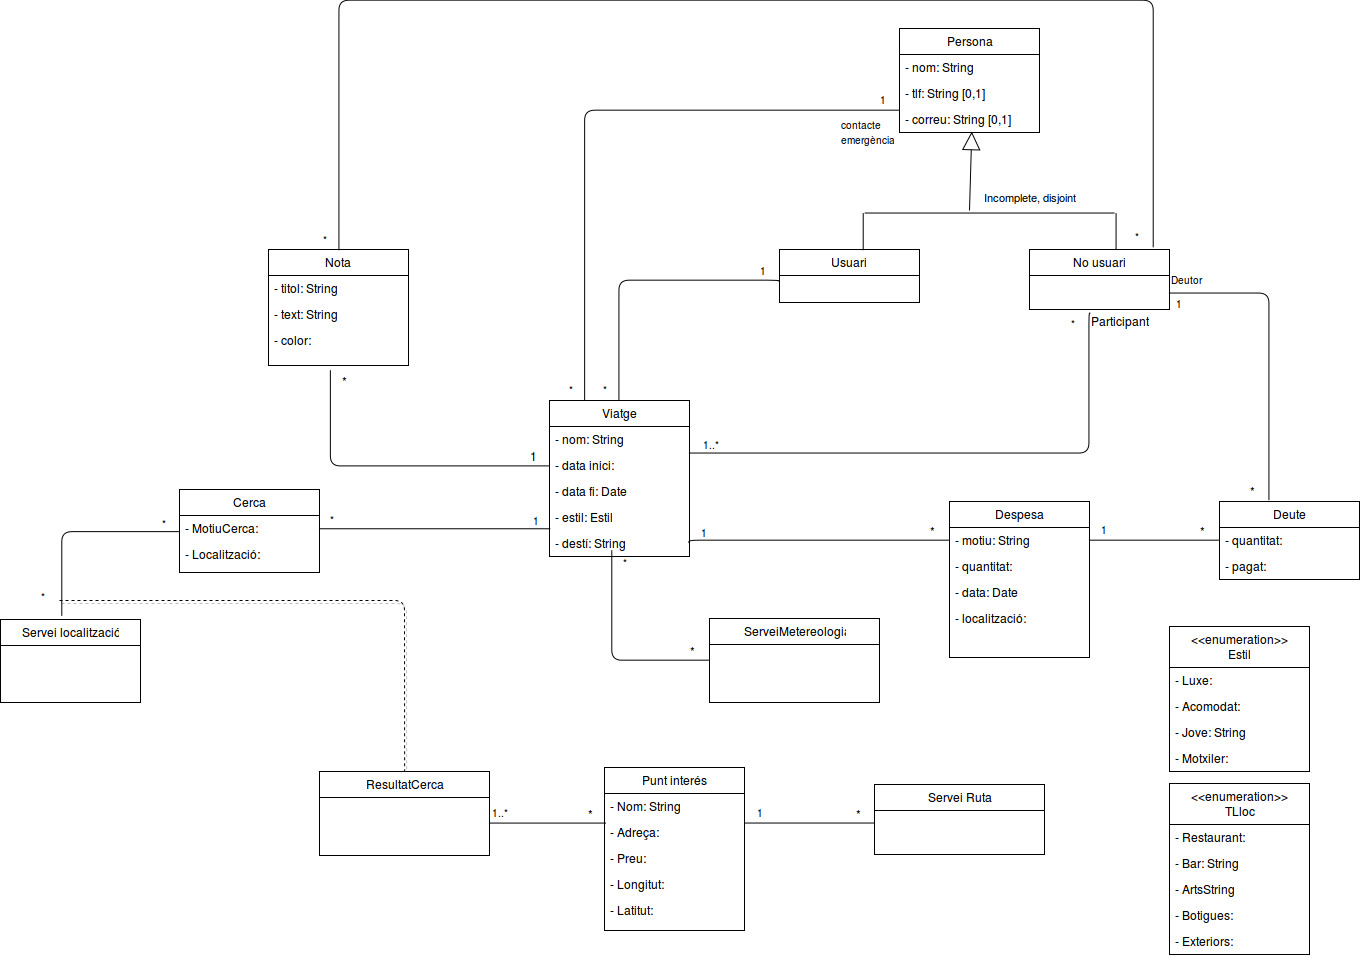
\includegraphics[scale=0.3]{Figures/UML.jpg}
\caption{Esquema conceptual.}
\end{figure}


\subsection{Restricions textuals}
\begin{itemize}
\item{}El deutor ha de ser participant del viatge al qual pertany el deute.
\item{}El viatger a qui se li comparteix una nota ha de ser participant del viatge al qual pertany la nota.
\end{itemize}

\clearpage

\subsection{Descripció de les entitats}

\newcolumntype{L}{>{\centering}m{4cm}}
\newcolumntype{M}{m{4cm}}
\newcolumntype{T}{m{7cm}}

\begin{itemize}

\item[]\textbf{Persona}\\
Super classe que s'instància per obtenir una persona de contacte.
\begin{table}[!h]
\begin{tabular}{|M|T|}
\hline
\textbf{Atribut}  & \textbf{Descripció} \\\hline
Nom &  Nom de la persona\\\hline
Tlf &  Telèfon de la persona\\\hline
Correu &  Correu electrònic de la persona\\\hline
\end{tabular}
\label{}
\caption{Atributs de la classe Persona}
\end{table}

\item[]\textbf{Usuari}\\
Té el rol d'usuari del sistema i és subclasse de Persona.
\begin{table}[!h]
\begin{tabular}{|M|T|}
\hline
\textbf{Atribut}  & \textbf{Descripció} \\\hline
Nom &  Nom de l'usuari\\\hline
Tlf &  Telèfon de l'usuari\\\hline
Correu &  Correu electrònic de l'usuari\\\hline
\end{tabular}
\label{}
\caption{Atributs de la classe Usuari}
\end{table}

\item[]\textbf{NoUsuari}\\
Té el rol de participant del viatge però sense ser usuari, no interacciona directament amb l'aplicació.

\begin{table}[!h]
\begin{tabular}{|M|T|}
\hline
\textbf{Atribut}  & \textbf{Descripció} \\\hline
Nom &  Nom del participant\\\hline
Tlf &  Telèfon del participant\\\hline
Correu &  Correu electrònic del participant\\\hline
\end{tabular}
\label{}
\caption{Atributs de la classe NoUsuari}
\end{table}

\item[]\textbf{Viatge}\\
Representa un viatge en concret, és el concepte base de l'aplicació.
\begin{table}[!h]
\begin{tabular}{|M|T|}
\hline
\textbf{Atribut}  & \textbf{Descripció} \\\hline
Nom &  Nom del viatge\\\hline
Destí &  Destí del viatge\\\hline
Data inici &  Data d'inici del viatge\\\hline
Data fi &  Data final del viatge\\\hline
Estil &  Estil de viatjar seleccionat per l'usuari\\\hline
\end{tabular}
\label{}
\caption{Atributs de la classe Viatge}
\end{table}

\clearpage

\item[]\textbf{Despesa}\\
Representa una despesa de l'usuari durant un viatge.

\begin{table}[!h]
\begin{tabular}{|M|T|}
\hline
\textbf{Atribut}  & \textbf{Descripció} \\\hline
Motiu &  Motiu de la despesa\\\hline
Quantitat &  Quantiat en euros de la despesa\\\hline
Localització &  Lloc on s'ha generat la despesa\\\hline
Data &  Data de creació de la despesa\\\hline
\end{tabular}
\label{}
\caption{Atributs de la classe Despesa}
\end{table}


\item[]\textbf{Deute}\\
Representa un deute d'un participant del viatge amb l'usuari.

\begin{table}[!h]
\begin{tabular}{|M|T|}
\hline
\textbf{Atribut}  & \textbf{Descripció} \\\hline
Quantitat & Quantitat del deute en euros.\\\hline
Pagat &  Indica si el deute ja ha estat pagat o no.\\\hline
\end{tabular}
\label{}
\caption{Atributs de la classe Deute}
\end{table}


\item[]\textbf{Nota}\\
Representa una nota escrita per l'usuari.

\begin{table}[!h]
\begin{tabular}{|M|T|}
\hline
\textbf{Atribut}  & \textbf{Descripció} \\\hline
Títol & Títol de la nota\\\hline
Text &  Text de la nota\\\hline
Color & Color que ha seleccionat l'usuari pel fons de la nota.\\\hline
\end{tabular}
\label{}
\caption{Atributs de la classe Nota}
\end{table}

\item[]\textbf{Cerca}\\
Representa una cerca llençada per l'usuari al sistema.

\begin{table}[!h]
\begin{tabular}{|M|T|}
\hline
\textbf{Atribut}  & \textbf{Descripció} \\\hline
Motiu & Tipus de cerca, aquest valor pot ser: menjar, begudes, arts, botigues o espais oberts\\\hline
Localització &  Localització des d'on es vol realitzar la cerca\\\hline
\end{tabular}
\label{}
\caption{Atributs de la classe Cerca}
\end{table}


\item[]\textbf{Servei Localització}\\
Representa el servei extern amb qui es comunica el sistema per obtenir resultats en la cerca.


\item[]\textbf{Resultat Cerca}\\
Representa els resultats d'una cerca en concret.

\item[]\textbf{Punt d'interés}\\
Representa un item concret del resultat de la cerca.

\begin{table}[!h]
\begin{tabular}{|M|T|}
\hline
\textbf{Atribut}  & \textbf{Descripció} \\\hline
Nom & Nom del punt d'interés\\\hline
Adreça &  Adreça del punt d'interés\\\hline
Preu & Nivell de preus del punt d'interés\\\hline
Latitut & Valor de latitut en la localització del punt d'interés\\\hline
Longitut & Valor de longitut en la localització del punt d'interés\\\hline
\end{tabular}
\label{}
\caption{Atributs de la classe Punt d'interés}
\end{table}


\item[]\textbf{Servei Ruta}\\
Representa el servei extern amb qui es comunica el sistema per tal d'obtenir una ruta entre dos punts.

\item[]\textbf{Servei Meteorologia}\\
Representa el servei extern amb qui es comunica el sistema per tal d'obtenir la previsió metereològica.



\end{itemize}

\section{Esquema del comportament}

\newcolumntype{C}{m{10cm}}

\begin{itemize}
\item[]{\textbf{Inici sessió}}

\begin{figure}[!h]
\centering
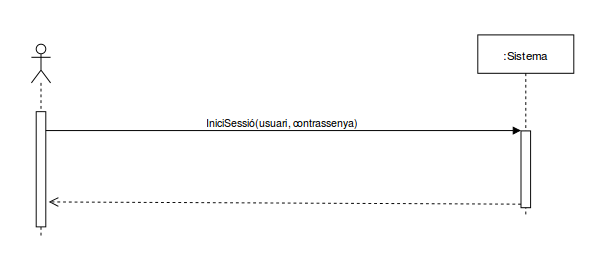
\includegraphics[scale=0.8]{Figures/IniciSessioEC.png}
\end{figure}

\begin{table}[!h]
\begin{tabular}{l C}
\textbf{Context}  & Sistema::IniciSessió(email:string, contrassenya:string) \\
\textbf{Pre} & email no és buit\\
 & contrassenya no es buida\\
\textbf{Post} &  Si les credencials són correctes l'usuari veu la pantalla de llista dels seus viatges\\
\end{tabular}
\label{}
\end{table}

\clearpage

\item[]{\textbf{Tancar sessió}}

\begin{figure}[!h]
\centering
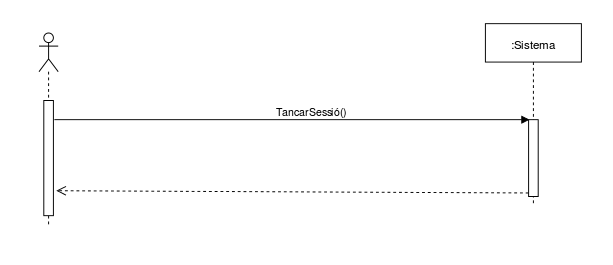
\includegraphics[scale=0.8]{Figures/TancarSessioEC.png}
\end{figure}

\begin{table}[!h]
\begin{tabular}{l C}
\textbf{Context}  & Sistema::TancarSessio() \\
\textbf{Pre} & L'usuari ha iniciat sessió\\
\textbf{Post} &  L'usuari veu la pantalla d'inici de sessió\\
\end{tabular}
\label{}
\end{table}

\item[]\textbf{Consultar viatge}

\begin{figure}[!h]
\centering
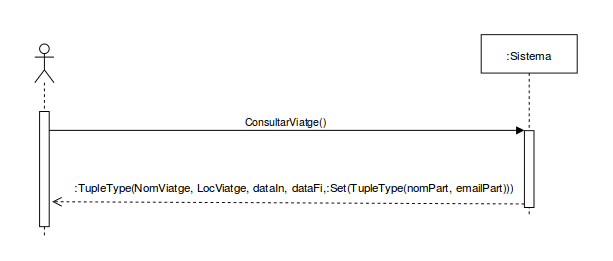
\includegraphics[scale=0.8]{Figures/ConsultarViatgeEC.png}
\end{figure}

\begin{table}[!h]
\begin{tabular}{l C}
\textbf{Context}  & Sistema::ConsultarViatge():TupleType(NomViatge, LocViatge, dataIn, dataFi,:Set(TupleType(nomPart, emailPart)) \\
\textbf{Pre} & L'usuari ha iniciat sessió\\
\textbf{Post} &  L'usuari veu la pantalla i les dades del viatge\\
\end{tabular}
\label{}
\end{table}

\clearpage

\item[]\textbf{Crear viatge}

\begin{figure}[!h]
\centering
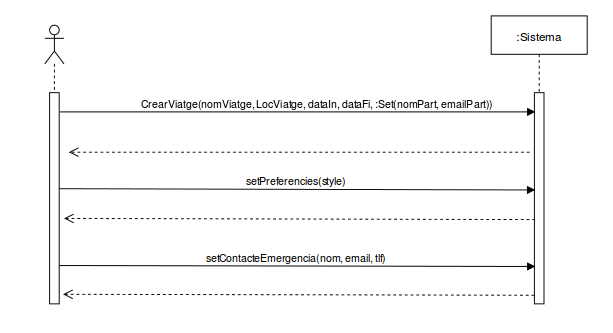
\includegraphics[scale=0.8]{Figures/CrearViatgeEC.png}
\end{figure}

\begin{table}[!h]
\begin{tabular}{l C}
\textbf{Context}  & Sistema::CrearViatge(nomViatge, LocViatge, dataIn, dataFi, :Set(nomPart, emailPart)) \\
\textbf{Pre} & L'usuari ha iniciat sessió\\
\textbf{Post} &  L'usuari veu la pantalla de seleccionar preferencies de viatge\\
\end{tabular}
\label{}
\end{table}

\begin{table}[!h]
\begin{tabular}{l C}
\textbf{Context}  & Sistema::SetPreferencies(estil) \\
\textbf{Pre} & L'usuari ha començat la creació d'un viatge\\
\textbf{Post} &  L'usuari veu la pantalla d'introduir les dades del contacte d'emergència\\
\end{tabular}
\label{}
\end{table}

\begin{table}[!h]
\begin{tabular}{l C}
\textbf{Context}  & Sistema::SetContactesEmergencia(nom, email, tlf) \\
\textbf{Pre} & L'usuari ha seleccionat les preferencies del viatge\\
\textbf{Post} &  S'ha creat el viatge amb totes les dades introduides\\
\end{tabular}
\label{}
\end{table}

\item[]\textbf{Eliminar viatge}

\begin{figure}[!h]
\centering
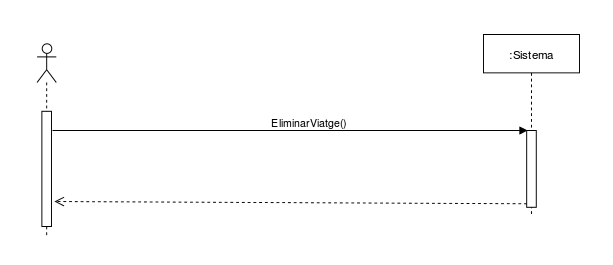
\includegraphics[scale=0.8]{Figures/EliminarViatgeEC.png}
\end{figure}

\clearpage

\begin{table}[!h]
\begin{tabular}{l C}
\textbf{Context}  & Sistema::EliminarViatge() \\
\textbf{Pre} & L'usuari ha creat un viatge\\
\textbf{Post} &  S'elimina el viatge amb totes les dades associades\\
\end{tabular}
\label{}
\end{table}



\item[]\textbf{Consultar llista de despeses}

\begin{figure}[!h]
\centering
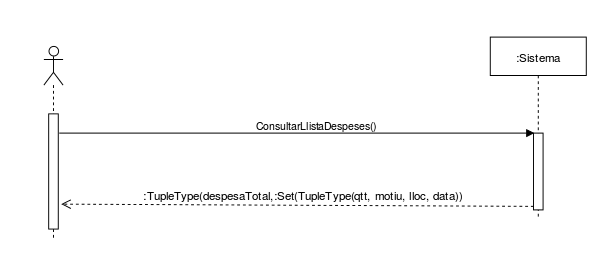
\includegraphics[scale=0.8]{Figures/ConsultarLlistaDespesesEC.png}
\end{figure}

\begin{table}[!h]
\begin{tabular}{l C}
\textbf{Context}  & Sistema::ConsultarLlistaDespeses():TupleType(despesaTotal,Set(TupleType(qtt, motiu, lloc, data)) \\
\textbf{Pre} & Ha accedit a consultar un viatge\\
\textbf{Post} &  L'usuari veu la pantalla amb la informació de totes les despeses del viatge\\
\end{tabular}
\label{}
\end{table}

\item[]\textbf{Crear despesa}


\begin{figure}[!h]
\centering
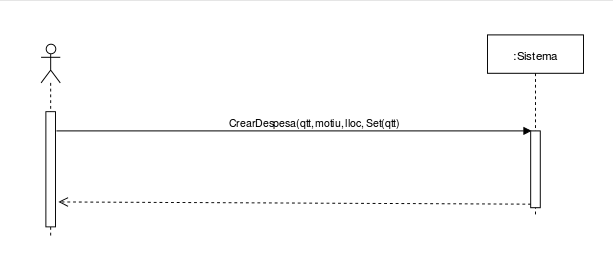
\includegraphics[scale=0.8]{Figures/CrearDespesaEC.png}
\end{figure}

\begin{table}[!h]
\begin{tabular}{l C}
\textbf{Context}  & Sistema::CrearDespesa(qtt, motiu, lloc, Set(qtt)) \\
\textbf{Pre} & Ha accedit a consultar la llista de despeses\\
\textbf{Post} & Es crea una instància de despesa amb les dades introduides\\
\end{tabular}
\label{}
\end{table}

\clearpage

\item[]\textbf{Consultar despesa}


\begin{figure}[!h]
\centering
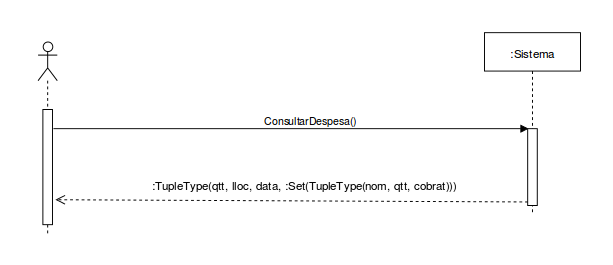
\includegraphics[scale=0.8]{Figures/ConsultarDespesaEC.png}
\end{figure}

\begin{table}[!h]
\begin{tabular}{l C}
\textbf{Context}  & Sistema::ConsultarDespesa()::TupleType(qtt, lloc, data, Set(TupleType(nom, qtt, cobrat))) \\
\textbf{Pre} & L'usuari ha creat una despesa\\
\textbf{Post} & L'usuari veu la pantalla de consultar despesa amb totes les dades d'aquesta\\
\end{tabular}
\label{}
\end{table}

\item[]\textbf{Cobrar deute}


\begin{figure}[!h]
\centering
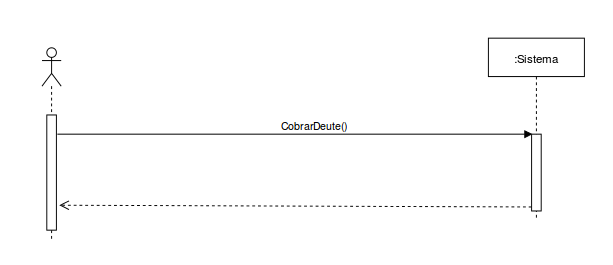
\includegraphics[scale=0.8]{Figures/CobrarDeuteEC.png}
\end{figure}

\begin{table}[!h]
\begin{tabular}{l C}
\textbf{Context}  & Sistema::CobrarDeute() \\
\textbf{Pre} & L'usuari ha creat una despesa i té un deute pendent de cobrar\\
\textbf{Post} & El sistema enregistra el deute com a cobrat\\
\end{tabular}
\label{}
\end{table}

\clearpage

\item[]\textbf{Eliminar despesa}


\begin{figure}[!h]
\centering
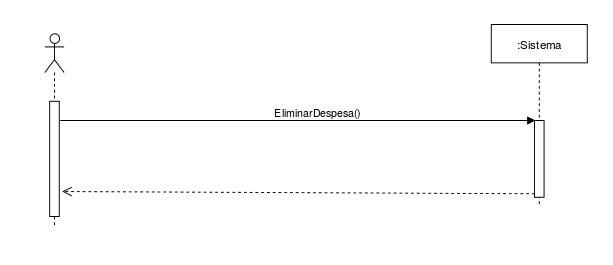
\includegraphics[scale=0.8]{Figures/EliminarDespesaEC.png}
\end{figure}

\begin{table}[!h]
\begin{tabular}{l C}
\textbf{Context}  & Sistema::EliminarDespesa() \\
\textbf{Pre} & L'usuari ha creat una despesa\\
\textbf{Post} & El sistema elimina la despesa i tots els deutes associats\\
\end{tabular}
\label{}
\end{table}

\item[]\textbf{Modificar despesa}


\begin{figure}[!h]
\centering
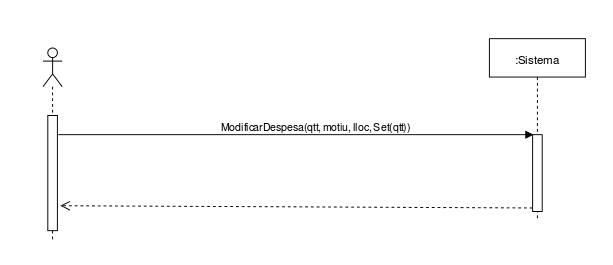
\includegraphics[scale=0.8]{Figures/ModificarDespesaEC.png}
\end{figure}

\begin{table}[!h]
\begin{tabular}{l C}
\textbf{Context}  & Sistema::ModificarDespesa(qtt, motiu, lloc, Set(qtt)) \\
\textbf{Pre} & L'usuari ha creat una despesa\\
\textbf{Post} & El sistema modifica la despesa amb els nous paràmetres introduits\\
\end{tabular}
\label{}
\end{table}

\clearpage

\item[]\textbf{Cerca}

\begin{figure}[!h]
\centering
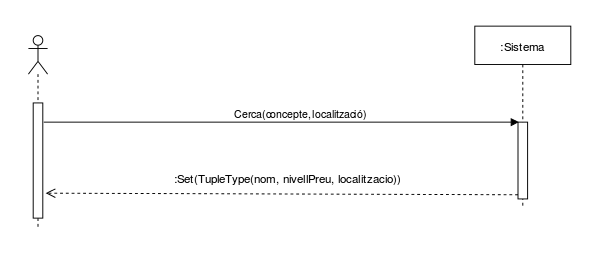
\includegraphics[scale=0.8]{Figures/CercaEC.png}
\end{figure}

\begin{table}[!h]
\begin{tabular}{l C}
\textbf{Context}  & Sistema::Cerca(concepte, localització):Set(TupleType(nom, nivellPreu, localitzacio)) \\
\textbf{Pre} & L'usuari ha accedit a consultar un viatge\\
\textbf{Post} & L'usuari veu la llista de resultats de la cerca\\
\end{tabular}
\label{}
\end{table}

\item[]\textbf{Consultar ruta}

\begin{figure}[!h]
\centering
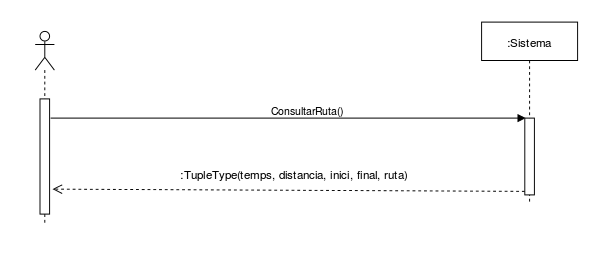
\includegraphics[scale=0.8]{Figures/ConsultarRutaEC.png}
\end{figure}

\begin{table}[!h]
\begin{tabular}{l C}
\textbf{Context}  & Sistema::ConsultarRuta():TupleType(temps, distancia, inici, final, ruta) \\
\textbf{Pre} & L'usuari ha realitzat una cerca\\
\textbf{Post} & L'usuari veu la pantalla de consultar ruta amb tota la informació de la ruta\\
\end{tabular}
\label{}
\end{table}

\clearpage

\item[]\textbf{Consultar Meteorologia}

\begin{figure}[!h]
\centering
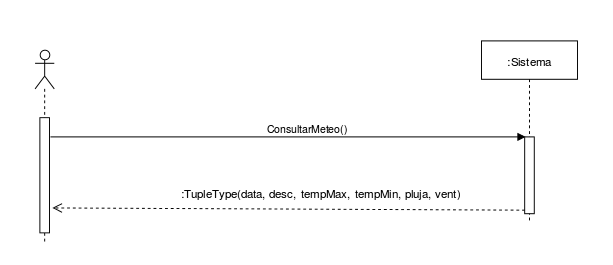
\includegraphics[scale=0.8]{Figures/ConsultarMeteoEC.png}
\end{figure}

\begin{table}[!h]
\begin{tabular}{l C}
\textbf{Context}  & Sistema::ConsultarMeteo():TupleType(data, desc, tempMax, tempMin, pluja, vent)\\
\textbf{Pre} & L'usuari ha accedit a consultar un viatge\\
\textbf{Post} & L'usuari veu la pantalla de consultar metereologia amb tota la informació de la previsió metereològica\\
\end{tabular}
\label{}
\end{table}

\item[]\textbf{Consultar ruta a l'hospital}

\begin{figure}[!h]
\centering
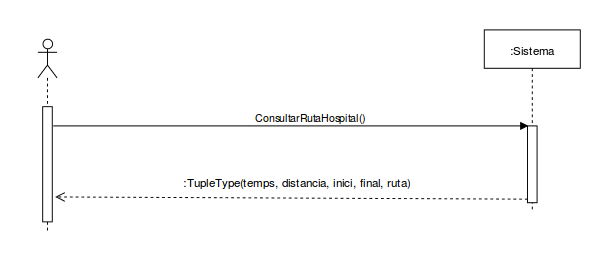
\includegraphics[scale=0.8]{Figures/ConsultarRutaHospitalEC.png}
\end{figure}

\begin{table}[!h]
\begin{tabular}{l C}
\textbf{Context}  & Sistema::ConsultarRutaHospital():TupleType(temps, distancia, inici, final, ruta)\\
\textbf{Pre} & L'usuari ha accedit a la funcionalitat de gestionar emergències\\
\textbf{Post} & L'usuari veu a la pantalla la ruta fins l'hospital més proper i tota la informació adicional\\
\end{tabular}
\label{}
\end{table}

\clearpage

\item[]\textbf{Trucar telèfon d'emergències}

\begin{figure}[!h]
\centering
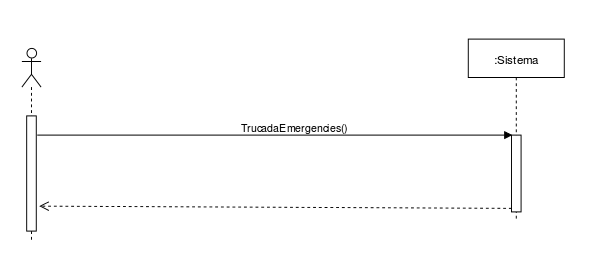
\includegraphics[scale=0.8]{Figures/TrucadaEmergenciesEC.png}
\end{figure}

\begin{table}[!h]
\begin{tabular}{l C}
\textbf{Context}  & Sistema::TrucadaEmergencies()\\
\textbf{Pre} & L'usuari ha accedit a la funcionalitat de gestionar emergències\\
\textbf{Post} & El sistema realitza una trucada al telèfon d'emergències del país on es troba l'usuari\\
\end{tabular}
\label{}
\end{table}

\item[]\textbf{Trucar telèfon de contacte}

\begin{figure}[!h]
\centering
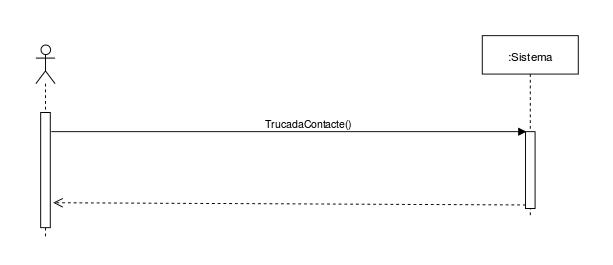
\includegraphics[scale=0.8]{Figures/TrucadaContacteEC.png}
\end{figure}

\begin{table}[!h]
\begin{tabular}{l C}
\textbf{Context}  & Sistema::TrucadaContacte()\\
\textbf{Pre} & L'usuari ha accedit a la funcionalitat de gestionar emergències\\
\textbf{Post} & El sistema realitza una trucada al telèfon de contacte introduit per l'usuari\\
\end{tabular}
\label{}
\end{table}

\clearpage

\item[]\textbf{Consultar llista de notes}

\begin{figure}[!h]
\centering
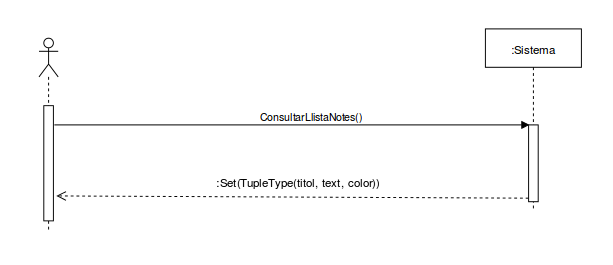
\includegraphics[scale=0.8]{Figures/ConsultarLlistaNotesEC.png}
\end{figure}

\begin{table}[!h]
\begin{tabular}{l C}
\textbf{Context}  & Sistema::ConsultarLlistaNotes():Set(TupleType(titol, text, color))\\
\textbf{Pre} & L'usuari ha accedit a consultar un viatge\\
\textbf{Post} & L'usuari veu la pantalla amb totes les notes del viatge\\
\end{tabular}
\label{}
\end{table}

\item[]\textbf{Consultar nota}

\begin{figure}[!h]
\centering
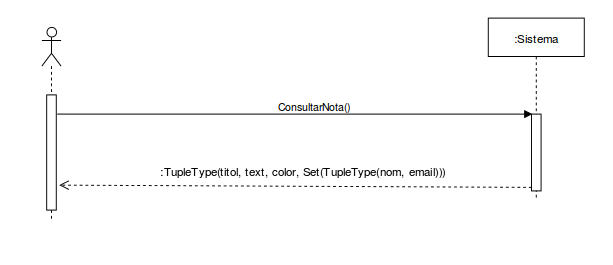
\includegraphics[scale=0.8]{Figures/ConsultarNotaEC.png}
\end{figure}

\begin{table}[!h]
\begin{tabular}{l C}
\textbf{Context}  & Sistema::ConsultarNota():TupleType(titol, text, color, Set(TupleType(nom, email)))\\
\textbf{Pre} & L'usuari ha consultar la llista de notes\\
\textbf{Post} & L'usuari veu la pantalla de consultar nota amb tota la informació d'aquesta\\
\end{tabular}
\label{}
\end{table}

\clearpage

\item[]\textbf{Crear nota}

\begin{figure}[!h]
\centering
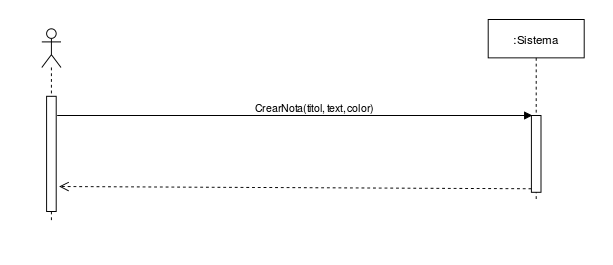
\includegraphics[scale=0.8]{Figures/CrearNotaEC.png}
\end{figure}

\begin{table}[!h]
\begin{tabular}{l C}
\textbf{Context}  & Sistema::CrearNota(titol, text, color)\\
\textbf{Pre} & L'usuari ha accedit a consultar la llista de notes\\
\textbf{Post} & El sistema crea una instància de nota amb les dades introduides i l'usuari veu la pantalla de consultar nota\\
\end{tabular}
\label{}
\end{table}

\item[]\textbf{Eliminar nota}

\begin{figure}[!h]
\centering
\includegraphics[scale=0.8]{Figures/EliminarNotaEC.png}
\end{figure}

\begin{table}[!h]
\begin{tabular}{l C}
\textbf{Context}  & Sistema::EliminarNota()\\
\textbf{Pre} & L'usuari ha accedit a consultar una nota\\
\textbf{Post} & El sistema elimina la nota\\
\end{tabular}
\label{}
\end{table}

\end{itemize}

% Chapter Template

\chapter{Disseny} % Main chapter title

\label{Disseny} % Change X to a consecutive number; for referencing this chapter elsewhere, use \ref{ChapterX}

Aquest projecte consta del desenvolupament d'una aplicació \textit{Android}, per aquest motiu l'arquitectura ha d'adaptar-se a les bones pràctiques d'aquesta plataforma.\\

El sistema separa clarament els conceptes en activitats diferents. Com que es tracta d'un dispositiu mòbil, aquestes activitats només són un llaç entre el sistema operatiu i l'aplicació, per tant, no sempre les controlem i en el cas que el dispositiu mòbil necessiti memòria pot eliminar l'activitat. Si separem els conceptes en activitats diferents minimitzem les dependències.

\section{Arquitectura}

Per al desenvolupament d'aquest projecte s'ha obtat per utilitzar l'arquitectura que proporciona la plataforma \textit{Android} per defecte. Aquesta consta d'un conjunt d'activitats que fan servir un model i controlen la interfície. En l'Activitat, només hi ha de constar el codi que faci de vincle entre el model i la vista, per aquest motiu, per tal de dur a terme tots els processos que es necessiten per obtenir la informació adequada s'ha dissenyat un servei (figura 8.1).

\begin{figure}[!h]
\centering
\includegraphics[scale=0.65]{Figures/ArquitecturaSistema.jpg}
\caption{Arquitectura de l'aplicació.}
\end{figure}

\begin{itemize}

\item[]{\textbf{Activitat}}\\
El sistema implementa una activitat per a cada funcionalitat diferent, d'aquesta manera, com s'ha exposat anteriorment, minimitzem les dependències i garantim més fiabilitat. No existeix un controlador que goberni les activitats sinó que es cada activitat que sap en tot moment amb qui s'ha de comunicar i qui pot ser que es comuniqui amb ella.\\

\item[]{\textbf{Servei}}\\
Des de qualsevol activitat es pot accedir a un servei per tal d'obtenir dades que es volen utilitzar per mostrar-les a l'usuari. En la figura 8.2 es pot apreciar una part de l'estructura dels serveis, es declara un servei per cada temàtica, dins el servei es dur a terme les operacions que convinguin utilitzant les dades guardades en els repositoris.

\begin{figure}[!h]
\centering
\includegraphics[scale=0.70]{Figures/EstructuraServeis.jpg}
\caption{Estructura dels serveis.}
\end{figure}

\item[]{\textbf{Dades}}\\
Es tenen en compte dos tipus de fonts de dades, les que guardem i consultem de la base de dades i les que obtenim de les consultes a serveis externs. Des del punt de vista de l'activitat, no hi ha cap diferencia en accedir-hi. \\
En el cas de les dades guardades a la base de dades, la qual està en el núvol, s'utilitzen uns repositoris per tal de tenir les dades en local. Hi ha un repositori per cada tipus d'entitat a la base de dades. En la figura 8.3 es pot apreciar l'accés des de l'activitat a la base de dades.\\
Pel que fa a les consultes a serveis externs no s'utilitzen respositoris, des del servei es fa una crida directament a la API corresponent per tal d'obtenir les dades i és al mateix servei on es tracten i es torna el resultat desitjat a l'activitat (figura 8.4).


\begin{figure}[!h]
\centering
\includegraphics[scale=0.6]{Figures/AccesBD.jpg}
\caption{Accés a les dades.}
\end{figure}

\begin{figure}[!h]
\centering
\includegraphics[scale=0.7]{Figures/AccesAPI.jpg}
\caption{Accés a serveis externs.}
\end{figure}

\clearpage

\end{itemize}


\subsection{Patrons de disseny}

En aquest apartat es descriuen els patrons utilitzats en el disseny del software. Com a primer plantejament, es va tenir en compte el patró Model-Vista-Controlador però això provoca que s'hagi de trencar el gran acoblament que ofereix la plataforma \textit{Android} entre el controlador i la vista. Per aquest motiu es va decidir decantar el disseny de l'arquitectura del projecte cap a l'estructura explicada en l'apartat anterior. Els patrons que es treballen en el projecte són els següents:
\begin{itemize}
\item{\textbf{Patró factoria}}\\
En el disseny de l'aplicació, s'utilitza el patró factoria per tal d'aconseguir els diferents tipus de servei. A més, això permet que en tot el sistema només existeixi una instància de cada servei i, per tant, a l'hora d'instanciar qualsevol servei s'ha de fer a través de la factoria.

\begin{figure}[!h]
\centering
\includegraphics[scale=0.75]{Figures/patroFactoria.png}
\caption{Patró factoria.}
\end{figure}

\item{\textbf{Patró adaptador}}\\
Per tal de cridar als serveis externs s'utilitza el patró adaptador, que fa de pont entre el servei i el sistema. Des de l'\textit{Activity} es crida a l'adaptador, i és l'adaptador qui es comunica amb el servei extern desitjat. D'aquesta manera aconseguim una capa d'abastracció que ens permetria canviar el servei extern i no haver de modificar res en l'\textit{Activity}.

\begin{figure}[!h]
\centering
\includegraphics[scale=0.75]{Figures/patroAdaptador.png}
\caption{Patró adaptador.}
\end{figure}

\clearpage

\item{\textbf{Patró repositori}}\\
S'utilitza per tal d'evitar l'accés directe a les dades i d'aquesta manera desacoblar al màxim l'accés a \textit{Firebase}. Per qualsevol classe que resulti un objecte emmagatzemat a la base de dades es definirà una interficie \textit{Repository} parametritzada, sobre la qual s'haurà de defnir una classe \textit{RepositoryXXXX} que la implementi.

\begin{figure}[!h]
\centering
\includegraphics[scale=0.75]{Figures/patroRepositori.png}
\caption{Patró repositori.}
\end{figure}

\item{\textbf{Patró servei}}\\
S'utilitza per crear una capa d'abstracció sobre els repositoris prèviament mencionats, cosa que permet desenvolupar en aquestes noves classes la lògica de l'aplicació sense accedir directament als repositoris. Aquests serveis contenen una instància única del repositori.

\begin{figure}[!h]
\centering
\includegraphics[scale=0.75]{Figures/patroServei.png}
\caption{Patró servei.}
\end{figure}

\end{itemize}

\subsection{Tecnologies utilitzades}
\begin{itemize}
\item[]{\textbf{Android}}\\
És el sistema operatiu per a dispositius mòbils amb pantalla tàctil més utilitzat. Actualment l'utilitzen des de telèfons inteligens i tables, fins a rellotges de nova generació, televisors i automòbils. És un projecte de codi obert recolçat per Google des del 2008. El desenvolupament d'aplicacions es fa habitualment en llenguatge Java i es diposa d'un SDK (Software Development Kit) que es pot descarregar gratuïtament des de la pàgina web oficial.\\

\item[]{\textbf{JSON}}\\
JavaScript Object Notation és el nom que rep una forma d'estructurar les dades per, posteriorment, ser enviades entre dispositius o per la xarxa. Es l'alternativa a XML en termes de llenguatge marcat i s'acostuma a utilitzar en les aplicacions Android per la comunicació amb el servidor o serveis externs.\\

\item[]{\textbf{Firebase}}\\
Firebase ofereix una base de dades en temps real com a servei. Aquest servei ofereix als desenvolupadors una API que permet guardar dades al núvol de les seves aplicacions. La companyia ofereix al client diverses llibreries per tal de facilitar la integració amb Android, iOS, Java i d'altres aplicacions.

\end{itemize}



\section{Capa de presentació}
\begin{itemize}

\item[]{\textbf{Iniciar sessió}}\\
El procés d'identificació de l'usuari es dur a terme a través de Google, per tant, l'usuari no es registra al nostre sistema sinó que utilitza les credencials del seu compte de Google per tal d'identificar-se.



\begin{figure}[!h]
\centering
\includegraphics[scale=0.15]{Figures/initSesion.png}
\includegraphics[scale=0.15]{Figures/TriarComte.png}
\caption{Inici de sessió}
\end{figure}

\item[]{\textbf{Consultar llista de viatges}}\\
A la pantalla de consultar viatges es mostra la llista de viatges de lúsuari. Si l'usuari selecciona qualsevol viatge l'aplicació el redigirà a la pantalla de consulta de viatge. També hi ha l'opció de crear un nou viatge. Des d'aquesta pantalla l'usuari pot tancar la sessió.

\clearpage

\begin{figure}[!h]
\centering
\includegraphics[scale=0.20]{Figures/llistaViatges.png}
\caption{Inici de sessió}
\end{figure}



\item[]{\textbf{Crear viatge}}\\
En aquesta pantalla és on s'introdueixen totes les dades d'un nou viatge com el nom, el destí, les dates i els participants. A més, el sistema li pregunta sobre el seu estil de viatjar i demana que li introdueixi les dades d'un contacte d'emergència. Un cop creat el viatge, l'aplicació redirigeix l'usuari a la pantalla de consultar viatge.



\begin{figure}[!h]
\centering
\includegraphics[scale=0.15]{Figures/cerarViatge.png}
\includegraphics[scale=0.15]{Figures/style.png}
\includegraphics[scale=0.15]{Figures/emergencyContact.png}
\caption{Crear viatge}
\end{figure}

\item[]{\textbf{Consultar viatge}}\\
La pantalla on es mostra tota la informació del viatge: nom, destí, dates i participants. A més, és la pantalla des d'on es pot accedir a totes les funcionalitats nombrades en apartats anteriors i permet eliminar el viatge.

\clearpage

\begin{figure}[!h]
\centering
\includegraphics[scale=0.15]{Figures/Drawer.png}
\includegraphics[scale=0.15]{Figures/getTrip.png}
\caption{Consultar viatge}
\end{figure}

\item[]{\textbf{Consultar llista de despeses}}\\
La pantalla de consultar despeses és on es poden veure totes les despeses del viatge i la quantitat total gastada. Si l'usuari selecciona una despesa el sistema el redirigeix a la pantalla de consultar despesa. A més, l'usuari també té l'opció de crear-ne una de nova, fet que el portarà a la pantalla de crear despesa.



\begin{figure}[!h]
\centering
\includegraphics[scale=0.15]{Figures/llistaDespeses.png}
\caption{Llista despeses}
\end{figure}

\item[]{\textbf{Crear despesa}}\\
En la pantalla crear despesa l'usuari introdueix les dades de la nova despesa com el motiu, la quantitat a pagar, la localització i si ha pagat una part a un company de viatge. Un cop creada la despesa el sistema redirigeix l'usuari a la pantalla de consultar despesa.

\clearpage

\begin{figure}[!h]
\centering
\includegraphics[scale=0.15]{Figures/crearDespesa.png}
\caption{Crear despesa}
\end{figure}

\item[]{\textbf{Consultar despesa}}\\
En la pantalla de consultar despesa l'usuari pot veure tota la informació de les despeses i té l'opció de marcar un deute com a pagat, modificar la despesa o eliminar-la. En el cas que l'usuari seleccioni modificar despesa el sistema el redirigeix a la pantalla de modificació de despesa, per l'altra banda, si decideix eliminar la despesa, el sistema el redirigeix a la pantalla de consultar llista de despeses.



\begin{figure}[!h]
\centering
\includegraphics[scale=0.15]{Figures/consultarDespesa.png}
\caption{Consultar despesa}
\end{figure}



\item[]{\textbf{Modificar despesa}}\\
En la pantalla de modificar despesa l'usuari pot modificar totes les dades d'una despesa. Quan comfirma la modificació el sistema el redirigeix la pantalla de consultar despesa.

\clearpage

\begin{figure}[!h]
\centering
\includegraphics[scale=0.15]{Figures/modificarDespesa.png}
\caption{Modificar despesa}
\end{figure}


\item[]{\textbf{Cerca llocs d'interés}}\\
En la pantalla de cerca lloc d'interés l'usuari pot seleccionar què vol buscar d'entre les possibilitats proposades i a quin lloc ho vol buscar. Si el lloc on ho vol buscar queda buit, es cercaran els resultats tenint en compte la localització de l'usuari en el moment de la cerca. Si no es troben resultats o es necessita activar el GPS s'informarà a l'usuari, d'altra banda, si la cerca es dur a terme satisfactoriament el sistema redirigirà l'usuari a la pantalla de llista de resultats de cerca.



\begin{figure}[!h]
\centering
\includegraphics[scale=0.15]{Figures/cerca.png}
\caption{Cerca de llocs d'interès}
\end{figure}



\item[]{\textbf{Consultar llista de resultats de cerca}}\\
És la pantalla on es veuen les resultats de la cerca, aquests estan ordenats per l'estil de viatjar de l'usuari. Per a cada item trobat es pot consultar el nom, la localització i, en cas que n'hi hagi, el nivell de preus de l'establiment. Quan l'usuari selecciona un resultat de la cerca el sistema el redirigeix a la pantalla de consultar ruta.

\clearpage

\begin{figure}[!h]
\centering
\includegraphics[scale=0.15]{Figures/resultatsCerca.png}
\caption{Resultats de cerca}
\end{figure}



\item[]{\textbf{Consultar ruta}}\\
En la pantalla de consultar ruta, l'usuari pot veure diverses opcions de ruta des d'on s'ha fet la cerca fins al punt seleccionat. A més, pot consultar la ruta en cotxe, transport públic i a peu, per a cada modalitat es poden veure paràmetres com la distància en quilòmetres i el temps que tardarà en arribar-hi. Si l'usuari prem sobre una de les rutes, l'aplicació li dona l'opció de consultar la ruta exacta utilitzant, en el cas que l'usuari la tingui instalada, l'aplicació Google Maps. Per últim, l'usuari té l'opció de consultar la ruta inversa.



\begin{figure}[!h]
\centering
\includegraphics[scale=0.15]{Figures/ruta.png}
\caption{Consultar ruta}
\end{figure}



\item[]{\textbf{Consultar previsió metereològica}}\\
En la pantalla de consultar previsió metereològica es pot veure la metereologia del dia actual amb paràmetre com la temperatura màxima i mínima, el percentatge de possibilitat de pluja, la velocitat del vent o la descripció del cel. A més, l'usuari també pot consultar la previsió fins a sis dies vista.

\clearpage

\begin{figure}[!h]
\centering
\includegraphics[scale=0.15]{Figures/meteo.png}
\caption{Previsió metereològica}
\end{figure}

\item[]{\textbf{Emergències}}\\
En la pantalla d'emergències l'usuari té tres opcions. La primera és realitzar una trucada al telèfon d'emergències del país on estigui, si selecciona aquesta opció el sistema el redirigirà a la pantalla de trucades del seu dispositiu mòbil. La segona opció es tracta de realitzar una trucada al seu propi contacte d'emergències, en aquest cas també se'l redirigirà a la pantalla de trucades del seu dispositiu mòbil. Per últim, té l'opció de seleccionar l'opció d'obtenir la ruta a l'hospital més proper, en aquest cas se'l redirigirà a la pantalla de consultar ruta.

\begin{figure}[!h]
\centering
\includegraphics[scale=0.15]{Figures/emergencies.png}
\includegraphics[scale=0.15]{Figures/hospital.png}
\caption{Gestió d'emergències}
\end{figure}

\clearpage

\item[]{\textbf{Consultar llista de notes}}\\
En aquesta pantalla l'usuari pot consultar la llista de notes que té el viatge. Des d'aquesta pantalla pot accedir a consultar una nota en concret o crear-ne una de nova.

\begin{figure}[!h]
\centering
\includegraphics[scale=0.15]{Figures/llistaNotes.png}
\caption{Llista de notes}
\end{figure}

\item[]{\textbf{Crear nota}}\\
En la pantalla de crear nota, l'usuari pot introduir el títol i el text de la nota i pot seleccionar un color per tal de canviar el fons d'aquesta. També pot seleccionar els participants del viatge amb qui vol compartir la nota a través de correu electrònic.


\begin{figure}[!h]
\centering
\includegraphics[scale=0.12]{Figures/crearNota1.png}
\includegraphics[scale=0.12]{Figures/crearNota2.png}
\includegraphics[scale=0.12]{Figures/crearNota3.png}
\includegraphics[scale=0.12]{Figures/crearNota4.png}
\caption{Crear nota}
\end{figure}



\item[]{\textbf{Consultar nota}}\\
En la pantalla de consultar nota l'usuari pot veure la nota seleccionada i té informació de amb qui l'ha compartit. A més, sempre pot canviar el color del fons de la nota.

\clearpage

\begin{figure}[!h]
\centering
\includegraphics[scale=0.15]{Figures/consultarNota.png}
\caption{Consultar nota}
\end{figure}


\end{itemize}

%\section{Canvis en les restriccions}

\section{Diagrama de classes de disseny}

\section{Model de dades}

En aquest apartat s'explica el model de dades utilitzat per desenvolupar el projecte. La base de dades que s'ha utilitzat és un base de dades no relacional de tipus \textit{key-value}. Per tal de modelar les dades, s'han seguit les bones pràctiques de la tecnologia utilitzada \textit{Firebase}.\\

Les dades del projecte es guarden en una direcció concreta que proporciona \textit{Firebase}. En aquesta direcció existeix un node pare del projecte des d'on pengen totes les dades. Des d'aquest node pare pengen llistes clau-valor, per cada tipus de dades diferent, amb totes les dades emmagatzemades d'aquell tipus concret (figura 8.25). El fet que es guardin les dades per tipus de d'entitat és degut a que els manuals de \textit{Firebase} defineixen que per tal d'obtenir un bon resultat és el camí que s'ha de seguir.

\begin{figure}[!h]
\centering
\includegraphics[scale=1.00]{Figures/EstructuraBD.jpg}
\caption{Estructura base de dades.}
\end{figure}


En la llista d'una entitat en concret, per a cada clau tenim un valor, i aquest valor conté tots els atributs de l'entitat guardada. En tenir llistes separades per cada entitat, quan es necessita referenciar un altre objecte guardat en la base de dades, s'utilitza la clau. Per tant, un deute no s'emmagatzema dins la despesa a la qual pertany sinnó que es guarda en la llista de deutes i es guarda un atribut amb la clau de la despesa (figura 8.26).


\begin{figure}[!h]
\centering
\includegraphics[scale=1.00]{Figures/DebtBD.jpg}
\caption{Solució per no duplicar informació.}
\end{figure}


\section{Diagrames de seqüència}

% Chapter Template

\chapter{Implementació} % Main chapter title

\label{Implementacio} % Change X to a consecutive number; for referencing this chapter elsewhere, use \ref{ChapterX}

En aquest apartat s'explica de quina manera s'han utilitzat les tecnologies seleccionades per al desenvolupament.

\begin{itemize}
\item{}\textbf{Inici de sessió}\\

Per a l'inici de sessió s'utilitza el servei que proporciona \textit{Google}. L'aplicació mostra a l'usuari el botó d'inici de sessió d'aquesta plataforma, quan es prem aquest botó es desvia l'inici de sessió a \textit{Google} (figura 9.1) on l'usuari introdueix les dades del seu compte.

\begin{figure}[!h]
\centering
\includegraphics[scale=0.9]{Figures/initSessio1.png}
\caption{Crida d'inici de sessió}
\end{figure}

Un cop l'usuari ha introduit les seves dades a \textit{Google} es retorna el control al sistema. Quan l'aplicació continua amb la seva execució ho fa a partir de la funció que es pot veure en la figura 9.2. L'últim pas per a l'inici de sessió es obtenir les dades de l'usuari i iniciar l'aplicació.

\begin{figure}[!h]
\centering
\includegraphics[scale=0.8]{Figures/initSessio2.png}
\caption{Retorn d'inici de sessió}
\end{figure}

\item{\textbf{Accés a la base de dades}}\\

La connexió amb la base de dades es dur a terme des de la classe \textit{FirebaseRepository}, aquesta classe és la classe genèrica que utilitzarant tots els serveis per tal d'accedir a la base de dades. En la figura 9.3 es pot veure com s'inicialitzen els camps del repositori.

\clearpage

\begin{figure}[!h]
\centering
\includegraphics[scale=0.8]{Figures/db1.png}
\caption{Constructor del repositori}
\end{figure}

Dins d'aquesta classe es defineixen totes les operacions que es poden fer sobre la base de dades. En la figura 9.4 es pot veure com es declara un \textit{insert}.

\begin{figure}[!h]
\centering
\includegraphics[scale=0.8]{Figures/db2.png}
\caption{Funció d'\textit{insert} genèrica}
\end{figure}

Per tal de llegir dades de firebase, el que es fa és el següent. Quan s'inicia l'aplicació es carreguen totes les dades de l'usuari en els repositoris. A més, per tal de tenir sempre els repositoris actualitzats, s'implementen \textit{listeners}. Quan es carreguen les dades provinents de \textit{Firebase} a les estructures del sistema es necessita convertir les dades del núvol en objectes del sistema. Per aquest motiu, s'utilitza la funció convert que es pot veure en la figura 9.5.

\begin{figure}[!h]
\centering
\includegraphics[scale=0.8]{Figures/db3.png}
\caption{Conversió de les dades a l'entitat Nota}
\end{figure}

\item{\textbf{Accés a les dades des de l'\textit{Activity}}}\\

Per interaccionar amb les dades i poder mostrar-les a l'usuari s'implementen diversos serveis. Aquests serveis són els encarregats de fer les operacions necessaries per tal de proporcionar a l'\textit{Activity} les dades que vol mostrar a l'usuari o per tal d'emmagatzemar les dades que l'usuari introdueix.\\

Es declara un servei per cada funcionalitat: un servei pels diferents tipus de persones, un per als viatges, un per despeses i deutes, i un altre per a les notes. En cada servei tenim una instància de repositori del tipus que estem tractant, per exemple, en el servei que tracta les despeses tenim una instància del repositori de despeses i una instància del repositori de deutes. En el servei es defineixen operacions com la de la figura 9.6.


\begin{figure}[!h]
\centering
\includegraphics[scale=0.8]{Figures/serv1.png}
\caption{Mètode de la classe ExpenseService}
\end{figure}

Pel que fa a l'\textit{Activity}, es declara el servei com en la figura 9.7 i s'utilitza aquest servei per tal d'obtenir qualsevol dada i guardar les dades introduides per l'usuari.

\begin{figure}[!h]
\centering
\includegraphics[scale=0.8]{Figures/serv2.png}
\caption{Mètode de la classe ExpenseService}
\end{figure}

\item{\textbf{Connexió amb serveis externs}}\\

En la connexió amb els serveis externs que s'utiltizen s'utilitza la mateixa arquitectura que en l'accés a les dades. Des del punt de vista de l'\textit{Activity}, el procediment és exactament el mateix. S'instància el servei que es necessita obtenint-lo de la factoria de serveis i s'utilitza per tal d'obtenir les dades que es necessiten.\\

La diferencia es veu en la classe servei, ja que enlloc de comunicar-se amb la base de dades es comunica amb un servei extern. En la figura 9.8 i 9.9 es pot veure un exemple de crida al servei extern que proporciona la llista dels hospitals que hi ha al voltant de l'usuari i posteriorment es selecciona el més proper a l'usuari. El resultat de la crida als diferents serveis sempre és un JSON el qual es deserialitza per tal d'obtenir objectes útils per al sistema.\\

\begin{figure}[!h]
\centering
\includegraphics[scale=0.8]{Figures/api2.png}
\caption{Mètode per obtenir l'hospital més proper}
\end{figure}

\begin{figure}[!h]
\centering
\includegraphics[scale=0.8]{Figures/api1.png}
\caption{Crida al servei de punts d'interés}
\end{figure}

\item{\textbf{Enviar correu electrònic}}\\

Per tal de poder enviar un correu electrònic directament des del codi \textit{Android} s'utilitza una classe anomenada MailSender. En aquesta classe es defineixen tots els paràmetres que permetran enviar un correu electrònic. En la figura 9.10 es pot veure el fragment de codi on es defineixen els paràmetre que permeten enviar des de \textit{Gmail}, s'inicia la sessió amb les credencials del compte \textit{WildTraveling} i es crea i envia el missatge en si.

\clearpage

\begin{figure}[!h]
\centering
\includegraphics[scale=0.8]{Figures/email.png}
\caption{Enviament d'un correu electrònic}
\end{figure}

Des de l'\textit{Activity}, per tal d'enviar un email, es crea una instància de la classe MailSender amb les dades del receptor del correu, l'assumpte i el cos, i s'executa el procés que s'ha definit dins la classe (Figura 9.11).

\begin{figure}[!h]
\centering
\includegraphics[scale=0.8]{Figures/email2.png}
\caption{Funció enviar correu electrònic}
\end{figure}

\end{itemize}
% Chapter Template

\chapter{Proves} % Main chapter title


\label{Proves} % Change X to a consecutive number; for referencing this chapter elsewhere, use \ref{ChapterX}

En aquest apartat es defineixen les proves que s'han fet sobre el sistema per tal d'assegurar un correcte funcionament.

\section{Proves de desenvolupament}

A continuació, es mostra per a cada cas d'ús, quines són les característiques que s'han de provar i el resultat esperat.

\begin{itemize}

\item{}\textbf{Registre i inici de sessió al sistema}

\begin{table}[!h]
\centering
\begin{tabular}{|T|T|}
\hline
\textbf{Característica} & \textbf{Resultat esperat} \\\hline
Connexió amb Google & Connexió satisfactòria\\\hline
\end{tabular}
\label{}
\caption{Proves \textit{Registrar-se al sistema}}
\end{table}

\item{}\textbf{Tancar sessió}

\begin{table}[!h]
\centering
\begin{tabular}{|T|T|}
\hline
\textbf{Característica} & \textbf{Resultat esperat} \\\hline
Des de la pantalla inicial, s'indica que es vol sortir. & Es mostra un diàleg de confirmació. Si s'accepta, es mostra la pantalla d'inici de sessió, si es cancel·la, es tanca el diàleg.\\\hline
\end{tabular}
\label{}
\caption{Proves \textit{Tancar sessió}}
\end{table}

\item{}\textbf{Crear viatge}

\begin{table}[!h]
\centering
\begin{tabular}{|T|T|}
\hline
\textbf{Característica} & \textbf{Resultat esperat} \\\hline
Algun camp és buit. & Es mostra un avís\\\hline
Les dades generals són correctes & Es mostra el diàleg de selecció d'estil.\\\hline
Es selecciona un estil de viatjar. & Si s'accepta, es mostra el diàleg d'introduir contacte d'emergència, si es cancel·la, es tanca el diàleg.\\\hline
Les dades del contacte d'emergència són correctes. & Es crea el viatge i es veu la pantalla de consultar el viatge.\\\hline
\end{tabular}
\label{}
\caption{Proves \textit{Crear viatge}}
\end{table}

\clearpage

\item{}\textbf{Consultar llista de viatges}

\begin{table}[!h]
\centering
\begin{tabular}{|T|T|}
\hline
\textbf{Característica} & \textbf{Resultat esperat} \\\hline
L'usuari no té viatges. & Es mostra la pantalla sense cap viatge.\\\hline
L'usuari té viatges creats. & Es mostra la llista de viatges.\\\hline
\end{tabular}
\label{}
\caption{Proves \textit{Consultar llista de viatges}}
\end{table}

\item{}\textbf{Consultar viatge}

\begin{table}[!h]
\centering
\begin{tabular}{|T|T|}
\hline
\textbf{Característica} & \textbf{Resultat esperat} \\\hline
Es prem el botó de tornar. & Es mostra la pantalla de llista de viatges.\\\hline
Es prem el botó de consultar despeses. & Es mostra la llista de despeses.\\\hline
Es prem el botó d'explorar. & Es mostra la pantalla de cerca de punts d'interès.\\\hline
Es prem el botó de previsió meteorològica. & Es mostra la previsió meteorològica.\\\hline
Es prem el botó d'emergències. & Es mostra la pantalla d'emergències.\\\hline
Es prem el botó de notes. & Es mostra la llista de notes.\\\hline
El viatge d'altres participants. & Es mostra la llista de participants.\\\hline
El viatge té tots els camps. & Es mostren les dades generals del viatge.\\\hline
\end{tabular}
\label{}
\caption{Proves \textit{Consultar viatge}}
\end{table}

\item{}\textbf{Consultar llista de despeses}

\begin{table}[!h]
\centering
\begin{tabular}{|T|T|}
\hline
\textbf{Característica} & \textbf{Resultat esperat} \\\hline
El viatge té despeses. & Es mostra la llista de despeses i el total acumulat.\\\hline
Es prem el botó de crear despesa. & Es mostra la pantalla de crear despesa.\\\hline
El viatge no té despeses. & Es mostra la pantalla sense cap despesa i el total cumulat a zero.\\\hline
\end{tabular}
\label{}
\caption{Proves \textit{Consultar llista de despeses}}
\end{table}

\item{}\textbf{Afegir nova despesa}

\begin{table}[!h]
\centering
\begin{tabular}{|T|T|}
\hline
\textbf{Característica} & \textbf{Resultat esperat} \\\hline
Algun camp és buit. & Es mostra un avís\\\hline
Les dades són correctes. & Es crea la despesa i es veu la pantalla de consultar la despesa.\\\hline
\end{tabular}
\label{}
\caption{Proves \textit{Afegir nova despesa}}
\end{table}

\clearpage

\item{}\textbf{Consultar despesa}

\begin{table}[!h]
\centering
\begin{tabular}{|T|T|}
\hline
\textbf{Característica} & \textbf{Resultat esperat} \\\hline
La despesa té tots els paràmetres. & Es mostren totes les dades de la despesa.\\\hline
La despesa té deutes associats. & Es mostra la llista de deutes.\\\hline
Es prem el botó de modificar despesa. & Es mostra la pantalla de modificar despesa.\\\hline
\end{tabular}
\label{}
\caption{Proves \textit{Consultar despesa}}
\end{table}

\item{}\textbf{Cobrar deute}

\begin{table}[!h]
\centering
\begin{tabular}{|T|T|}
\hline
\textbf{Característica} & \textbf{Resultat esperat} \\\hline
L'usuari prem mantingudament un deute. & Es mostra un diàleg de confirmació. Si s'accepta, es marca el deute com a pagat, si es cancel·la, es tanca el diàleg.\\\hline
\end{tabular}
\label{}
\caption{Proves \textit{Cobrar deute}}
\end{table}

\item{}\textbf{Modificar despesa}

\begin{table}[!h]
\centering
\begin{tabular}{|T|T|}
\hline
\textbf{Característica} & \textbf{Resultat esperat} \\\hline
L'usuari modifica algun paràmetre. & Es mostra el paràmetre modificat.\\\hline
L'usuari prem el botó de tornar. & Es guarden tots els canvis i es mostra un avís.\\\hline
\end{tabular}
\label{}
\caption{Proves \textit{Modificar despesa}}
\end{table}

\item{}\textbf{Eliminar despesa}

\begin{table}[!h]
\centering
\begin{tabular}{|T|T|}
\hline
\textbf{Característica} & \textbf{Resultat esperat} \\\hline
L'usuari prem el botó d'eliminar despesa. & Es mostra un diàleg de confirmació. Si s'accepta s'elimina la despesa i es mostra la llista de despeses, si es cancel·la es tanca el diàleg.\\\hline
\end{tabular}
\label{}
\caption{Proves \textit{Eliminar despesa}}
\end{table}

\item{}\textbf{Gestionar cerques}

\begin{table}[!h]
\centering
\begin{tabular}{|T|T|}
\hline
\textbf{Característica} & \textbf{Resultat esperat} \\\hline
L'usuari prem el botó de gestionar cerques. & Es mostra la pantalla de realitzar cerca.\\\hline
\end{tabular}
\label{}
\caption{Proves \textit{Gestionar cerques}}
\end{table}

\clearpage

\item{}\textbf{Realitzar cerca}

\begin{table}[!h]
\centering
\begin{tabular}{|T|T|}
\hline
\textbf{Característica} & \textbf{Resultat esperat} \\\hline
L'usuari selecciona un item a buscar. & Es mostra el nom de l'item a buscar.\\\hline
L'usuari prem el botó d'explorar. & Es realitza la cerca. Si l'usuari ha introduït localització es busca sobre la introduïda, si no n'ha introduït es busca sobre la localització real de l'usuari.Finalment es mostra la pantalla dels resultats amb tota la informació i ordenats per nivell de preu.\\\hline
No hi ha resultats de cerca & Es mostra un avís.\\\hline
\end{tabular}
\label{}
\caption{Proves \textit{Realitzar cerca}}
\end{table}

\item{}\textbf{Consultar ruta}

\begin{table}[!h]
\centering
\begin{tabular}{|T|T|}
\hline
\textbf{Característica} & \textbf{Resultat esperat} \\\hline
L'usuari selecciona un item de la llista de resultats. & Es mostra la pantalla de consultar ruta amb la informació sobre el mapa de la ruta a peu, la distància i el temps.\\\hline
L'usuari selecciona la ruta amb vehicle. & Es mostra la pantalla de consultar ruta amb la informació sobre el mapa de la ruta amb vehicle, la distància i el temps.\\\hline
L'usuari selecciona el canvi de sentit de la ruta & Es mostra la pantalla de consultar ruta amb la informació sobre la nova ruta.\\\hline
\end{tabular}
\label{}
\caption{Proves \textit{Consultar ruta}}
\end{table}

\item{}\textbf{Consultar previsió meteorològica}

\begin{table}[!h]
\centering
\begin{tabular}{|T|T|}
\hline
\textbf{Característica} & \textbf{Resultat esperat} \\\hline
L'usuari prem el botó de consultar previsió meteorològica. & Es mostra la informació de la previsió meteorològica la informació actualitzada.\\\hline
\end{tabular}
\label{}
\caption{Proves \textit{Consultar previsió meteorològica}}
\end{table}

\item{}\textbf{Gestionar emergències}

\begin{table}[!h]
\centering
\begin{tabular}{|T|T|}
\hline
\textbf{Característica} & \textbf{Resultat esperat} \\\hline
L'usuari prem el botó de gestionar emergències. & Es mostra la pantalla de gestionar emergències.\\\hline
\end{tabular}
\label{}
\caption{Proves \textit{Gestionar emergències}}
\end{table}

\clearpage

\item{}\textbf{Trucar telèfon d'emergència}

\begin{table}[!h]
\centering
\begin{tabular}{|T|T|}
\hline
\textbf{Característica} & \textbf{Resultat esperat} \\\hline
L'usuari prem el botó de trucar al telèfon d'emergències. & S'inicia una trucada amb el telèfon d'emergències.\\\hline
\end{tabular}
\label{}
\caption{Proves \textit{Trucar telèfon d'emergències}}
\end{table}

\item{}\textbf{Trucar telèfon de contacte}

\begin{table}[!h]
\centering
\begin{tabular}{|T|T|}
\hline
\textbf{Característica} & \textbf{Resultat esperat} \\\hline
L'usuari prem el botó de trucar al telèfon de contacte. & S'inicia una trucada amb el telèfon de contacte.\\\hline
\end{tabular}
\label{}
\caption{Proves \textit{Trucar telèfon de contacte}}
\end{table}

\item{}\textbf{Consultar ruta a l'hospital}

\begin{table}[!h]
\centering
\begin{tabular}{|T|T|}
\hline
\textbf{Característica} & \textbf{Resultat esperat} \\\hline
L'usuari prem el botó de consultar ruta a l'hospital. & Es mostra la pantalla de consultar ruta amb la informació sobre el mapa de la ruta a peu a l'hospital més proper, la distància i el temps.\\\hline
\end{tabular}
\label{}
\caption{Proves \textit{Consultar ruta a l'hospital}}
\end{table}

\item{}\textbf{Consultar llista de notes}

\begin{table}[!h]
\centering
\begin{tabular}{|T|T|}
\hline
\textbf{Característica} & \textbf{Resultat esperat} \\\hline
El viatge no té notes. & Es mostra la pantalla de llistar notes sense cap nota.\\\hline
El viatge conté notes. & Es mostra la llista de notes.\\\hline
\end{tabular}
\label{}
\caption{Proves \textit{Consultar llista de notes}}
\end{table}

\item{}\textbf{Crear nota}

\begin{table}[!h]
\centering
\begin{tabular}{|T|T|}
\hline
\textbf{Característica} & \textbf{Resultat esperat} \\\hline
Algun camp és buit. & Es mostra un avís.\\\hline
L'usuari selecciona un color. & Es tenyeix el fons de la nota amb el color seleccionat.\\\hline
L'usuari comparteix la nota amb algun participant del viatge. & Es mostra el nom i el correu electrònic del participant amb qui s'ha compartit la nota.\\\hline
L'usuari prem el botó de crear la nota & Es crea la nota, s'envia un correu amb el contingut de la nota als participants amb qui s'ha compartit la nota i es veu la pantalla de consultar la nota creada.\\\hline
\end{tabular}
\label{}
\caption{Proves \textit{Crear nota}}
\end{table}

\clearpage

\item{}\textbf{Consultar nota}

\begin{table}[!h]
\centering
\begin{tabular}{|T|T|}
\hline
\textbf{Característica} & \textbf{Resultat esperat} \\\hline
La nota està compartida. & Es mostra la llista de viatgers amb qui s'ha compartit la nota.\\\hline
L'usuari selecciona un color. & Es tenyeix el fons de la nota amb el color seleccionat.\\\hline
\end{tabular}
\label{}
\caption{Proves \textit{Consultar nota}}
\end{table}

\item{}\textbf{Eliminar nota}

\begin{table}[!h]
\centering
\begin{tabular}{|T|T|}
\hline
\textbf{Característica} & \textbf{Resultat esperat} \\\hline
L'usuari prem el botó d'eliminar nota & Es mostra un diàleg de confirmació. Si s'accepta s'elimina la nota i es mostra la llista de notes, si es cancel·la es tanca el diàleg.\\\hline
\end{tabular}
\label{}
\caption{Proves \textit{Eliminar nota}}
\end{table}

\end{itemize}

Per a tots els casos d'ús, es comprova que les dades apareguin a la pantalla amb el format correcte i sense errors. A més, en molts punts es guarden dades a la base de dades remota, es comprova també que aquest emmagatzematge sigui correcte.

\section{Proves finals}

Les proves finals són el pas previ al llançament de l'aplicació al mercat. Per aquest motiu, s'ha demanat a un conjunt d'usuaris que utilitzin l'aplicació en els seus viatges. El \textit{feedback} rebut per part dels usuaris després de provar WildTraveling es pot resumir de la següent manera:
\begin{itemize}
\item{}Els usuaris opinen que l'aplicació és molt fàcil d'utilitzar i la interfície és molt elegant i senzilla.
\item{}Els usuaris no han tingut problemes en identificar les funcionalitats.
\item{}En la funcionalitat de cercar punts d'interès, alguns usuaris han trobat que la selecció de la localització no queda clara, ja que si el camp es deixa buit significa que s'utilitza la localització real de l'usuari.
\item{}A l'hora de crear una nova despesa, alguns usuaris han senyalat que si el viatge que dus a terme té molts participants, quan s'afegeixen deutes a la despesa estaria bé una opció que permeti afegir la mateixa quantitat a tots els participants.
\item{}Els usuaris han comprovat que l'aplicació és ràpida i no té problemes d'execució.
\end{itemize}

La valoració dels usuaris es considera molt bona, ja que han donat molta importància a la facilitat d'ús d'aquesta i a un disseny elegant i senzill. A més els petits inconvenients que han pogut identificar comporten canvis molt concrets en el sistema que es poden solucionar fàcilment de cara a pròximes actualitzacions i, en cap cas, aquests inconvenients comprometen el correcte funcionament del software.
% Chapter Template

\chapter{Informe de sostenibilitat} % Main chapter title

\label{InformeSostenbilitat} % Change X to a consecutive number; for referencing this chapter elsewhere, use \ref{ChapterX}

Per tal d’evaluar la sostenibilitat del projecte a nivel econòmic, social i ambiental es fabrica la matriu de sostenibilitat, on s’atribueix a cada dimensió un
valor evaluant així cada aspecte.\\


\begin{table}[!h]
\centering
\begin{tabular}{|l|r|}
\hline
\textbf{Caràcter}  & \textbf{Valoració} \\\hline
Econòmic & 8 \\\hline
Social & 8 \\\hline
Ambiental & 7 \\\hline
\textbf{Total} & 23 \\\hline
\end{tabular}
\label{}
\caption{Matriu de sostenibilitat}
\end{table}

\section{Dimensió econòmica}
Per aquest projecte s’han avaluat detalladament els costos tant de recursos com
materials. No s’han tingut en compte els costos deguts a possibles ajustaments,
reparacions o actualitzacions durant el desenvolupament ja que es tracta d’un
projecte acadèmic. Sí que es cert que es podria desenvolupar el mateix projecte
en menys temps, però per fer-ho possible es necessitaria més recursos humans
i d’una major experiència professional. Pel que fa a la planificació es pot assegurar que les tasques en les que s’ha dedicat més hores són les més importants.
Podem dir que que el cost total del projecte ha estat ajustat al màxim tenint en
compte els costos de projectes de desenvolupament de software similars, i això
converteix el sistema en un producte competitiu.

\section{Dimensió social}

El producte resultant d’aquest projecte facilitarà molt la vida a tots els viatgers
que vulguin un suport per tal de millorar les condicions del viatge. La necessitat del productes és real ja que sense ell el viatger es veu més confús a l’hora
d’obtenir informació sobre l’entorn degut a que les aplicacions existents són
molt específiques i no s’adapten a la necessitat de l’usuari.

\clearpage
\section{Dimensió ambiental}
El desenvolupament del projecte provoca la utilització de diversos recursos
que afecte el medi ambient. En les diferents parts del projecte s’utilitza l’energia elèctrica com a font d’energia per poder treballar, el cost d’aquesta té un
impacte ambiental. En concret s’utilitzarà l’energia elèctrica necessària per alimentar l’ordinador que s’utilitza per a desenvolupar i el dispositiu mòbil on
es fan les proves. A més, s’ha de tenir en compte també que per utilitzar l’aplicació és necessari tenir connexió a internet, cosa que també suposa un cost
elèctric.\\


Amb aquest nou producte, podem dir que es minimitzaran les descàrregues
de múltiples aplicacions, cosa que disminueix el cost elèctric. A més, també
promou l’estalvi de paper en termes de guies de turisme i altres.
	

% Chapter Template

\chapter{Conclusions} % Main chapter title

\label{Conclusions} % Change X to a consecutive number; for referencing this chapter elsewhere, use \ref{ChapterX}

\section{Justificació del desenvolupament de les competències tècniques}

\begin{itemize}
\item{}\textbf{CES1.1:} Desenvolupar, mantenir i avaluar sistemes i serveis software complexos i/o crítics. [En profunditat]\\
S’ha desenvolupat un sistema software de certa complexitat ja que incorpora funcionalitats molt diverses i no trivials.
\item{}\textbf{CES1.2:} Donar solució a problemes d’integració en funció de les estratègies, dels estàndards i de les tecnologies disponibles. [Bastant]\\
L’aplicació necessita de la participació d’aplicacions externes per tal d’aconseguir certes funcionalitats, per tant, s’ha fet un treball d’integració de
serveis externs. A través de l’ús de patrons, s’ha aconseguit obtenir un
sistema molt flexible a l’hora d’adjuntar nous serveis externs o elminar
els utilitzats.
\item{}\textbf{CES1.3:} Identificar, avaluar i gestionar els riscos potencials associats a la
construcció de software que es poguessin presentar. [Bastant]\\
S’han identificat els principals riscos a l’hora de desenvolupar el software
com, per exemple, la necessitat de connexió a internet. Un cop identificats
s’han evaluat i s’han gestionat de la millor manera possible aconseguint
així un bon funcionament del software i una reducció de les possibilitats
de fallada.
\item{}\textbf{CES1.5:} Especificar, dissenyar, implementar i avaluar bases de dades. [En profunditat]\\
S’ha dut a terme un anàlisi profund estudiant quin seria el millor disseny
per a la base de dades. S’ha obtat per utilitzar una tecnologia que no es
tracta durant els cursos del grau i, per tant, s’ha hagut de fer un esforç en l’aprenentatge de l’ús correcte d’aquesta.
\item{}\textbf{CES1.6:} Administrar bases de dades (CIS4.3) [Una mica]\\
L’administració de la base de dades té lloc un cop l’aplicació està posada
en marxa, per aquest motiu la competència no incideix molt en el treball
final de grau. Tot i així, si que es fa un treball sobre la base de dades durant la fase de proves.
\item{}\textbf{CES1.7:} Controlar la qualitat i dissenyar proves en la producció de software. [Bastant]\\
S’han dut a terme proves durant el desenvolupament del software. Les
proves han estat fetes pel desenvolupador i per usuaris externs al projecte
que han provat l’aplicació.
\item{}\textbf{CES1.9:} Demostrar comprensió en la gestió i govern dels sistemes software. [En profunditat]\\
Desenvolupar una aplicació com aquesta requereix d’una bona gestió del
sistema software i així ha estat. S’ha gestionat el sistema de manera correcta analizant varies alternatives i seleccionant la més adient.
\item{}\textbf{CES2.1:} Definir i gestionar els requisits d’un sistema software. [En profunditat]\\
En la fase inicial, es van definir tots els requisits de l’aplicació. Aquest punt del projecte és bàsic per al correcte desenvolupament de l’aplicació ja que es necessita saber què es vol fer, per aquest motiu és una competència que es treballa en profunditat.
\item{}\textbf{CES2.2:} Dissenyar solucions apropiades en un o més dominis d’aplicació, utilitzant mètodes d’enginyeria del software que integrin aspectes ètics, socials, legals i econòmics. [En profunditat]\\
El desenvolupament de l’aplicació té un impacte en la societat, a més, s’han identificat les lleis i restriccions que ha de complir el projecte. També s’ha evaluat la sostenibilitat del projecte en termes socials, econòmics i medioambientals.
\end{itemize}

\section{Desviacions en la planificació i el pressuposst}

En aquest apartat s’exposen les diferències que hi ha hagut entre la planificació inicial i la realitat en el desenvolupament del projecte i les conseqüències
d’aquestes desviacions sobre el pressupost.\\

\textbf{Fase inicial:}\\
La fase inicial ha estat més llarga del que s’esperava ja que es va haver de dedicar més hores de les previstes en la definició del projecte i l’especificació de
requisits. Això va comportar un retard de 7 dies.\\

\textbf{Iteracions:}\\
Degut al retard en la fase inicial, les iteracions es van començar una setmana després de l’esperat. Aquest fet va forçar una reorganització de la fase de
desenvolupament del producte. S’han convertit les 5 iteracions planificades en
7, fent-les més curtes.\\
A més, durant aquest periode s’ha hagut de posar més hores de feina de les
previstes degut a que es va planificar menys feina de la que hi havia.
\begin{itemize}
\item{}\textbf{Iteració 1:} 4 d’abril - 18 d’abril (planificació: 29 de març - 12 d’abril)\\
La primera iteració ha estat de dues setmanes ja que és un punt del pro-
jecte on s’ha de posar en marxa molts aspectes.
\item{}\textbf{Iteració 2:} 19 d’abril - 25 d’abril (planificació: 13 d’abril - 26 d’abril)\\
A partir d’aquesta iteració, ja es va decidir posar deadlines més propers
ja que el temps disponible ho forçava i la quantitat de feina a fer ho per-
metia.
\item{}\textbf{Iteració 3:} 26 d’abril - 2 de maig (planificació: 27 d’abril - 10 de maig)
\item{}\textbf{Iteració 4:} 3 de maig - 11 de maig (planificació : 11 de maig - 24 de maig)
\item{}\textbf{Iteració 5:} 11 de maig - 18 de maig (planificació: 25 de maig - 7 de juny)
\item{}\textbf{Iteració 6:} 19 de maig - 25 de maig (iteració extra)
\textbf{Iteració 7:} 26 de maig - 7 de juny (iteració extra)\\
En aquesta iteració es té previst millorar les interfícies i acabar alguns detalls pendents. Un cop finalitzada aquesta iteració el producte estarà llest
per ser llençat al mercat.
\end{itemize}

\textbf{Fase final}\\
La fase final no es veurà afectada pels canvis en la planificació que hi ha hagut en les fases anteriors.\\

Tenint en compte les desviacions mencionades, les hores emprades en el projecte queden repartides de la següent manera.

\begin{table}[!h]
\centering
\begin{tabular}{|l|c|r|}
\hline
\textbf{Fase}  & \textbf{Duració} & \textbf{\%} \\\hline
Fase incial & 119h & 36\% \\\hline
Iteracions & 169h & 51\% \\\hline
Fase final & 45h & 13\% \\\hline
\textbf{Total} & \textbf{333h}  & \textbf{100\%} \\\hline
\end{tabular}
\label{}
\caption{Distribució d'hores reals i percentatge de treball}
\end{table}

Per tant, hi ha una desviació de 76 hores que significa una diferència del 22\%. Aquest valor és força gran i es pot considerar que la planificació no va ser del
tot bona degut a la poca experiència en aquest camp.\\

Tal i com es va especificar a l’apartat de control de gestió, un cop acabat el projecte es contabilitzen les hores de treball que cada rol ha dedicat i es comparen amb les que s’havia planificat. El resultat obitngut és el que es mostra en la
taula 12.2.\\

El cost real del projecte, per tant, disminueix fins a 10.810\euro, un cost notablement inferior al planificat. Això és degut a que s’ha treballat menys hores de
les esperades i, els rols que han superat les hores planificades són rols de més
baixa retribució com el programador.

\begin{table}[!h]
\centering
\begin{tabular}{|c|c|c|c|c|c|}
\hline
\textbf{Rol}  & \textbf{Hores estimades} & \textbf{Cost estimat} & \textbf{Hores reals} & \textbf{Cost real}   \\ \hline
Cap de projecte & 160h & 7.200\euro & 126h & 5.670\euro \\\hline
Analista & 45h & 1.350\euro & 30h & 900\euro \\\hline
Dissenyador & 70h & 2.100\euro & 23h & 690\euro \\\hline
Programador & 104h & 2.600\euro & 124h & 3.100\euro \\\hline
Tester & 30h & 450\euro & 30h & 450\euro \\\hline
\end{tabular} 
\label{}
\caption{Comparativa entre les hores estimades i les reals treballades, i el seu cost associat}
\end{table}

En quant a les previsions de les despeses generals han seguit els valors que es
van preveure. Si restem els costos dels imprevistos i el valor de les contingències, el valor real del projecte és 11.000\euro.

\section{Gantt final}

\section{Limitacions i dificultats}

\section{Treball futur}


%----------------------------------------------------------------------------------------
%	THESIS CONTENT - APPENDICES
%----------------------------------------------------------------------------------------

\appendix % Cue to tell LaTeX that the following "chapters" are Appendices

% Include the appendices of the thesis as separate files from the Appendices folder
% Uncomment the lines as you write the Appendices

%\include{Appendices/AppendixA}
%\include{Appendices/AppendixB}
%\include{Appendices/AppendixC}

%----------------------------------------------------------------------------------------
%	BIBLIOGRAPHY
%----------------------------------------------------------------------------------------

\printbibliography[heading=bibintoc]

%----------------------------------------------------------------------------------------

\end{document}  
